\documentclass{article}
\usepackage{setspace}
\usepackage[explicit]{titlesec}
\usepackage{forest}
\usepackage{hyperref}
\usepackage{graphicx}
\usepackage{listings}
% Used for creating clean tables within app
\usepackage{booktabs}
% Used for creating check marks in app, amongst others
\usepackage{amssymb}
% Used for creating gray color background boxes
\usepackage[breakable, theorems, skins]{tcolorbox}
% dirtytalk is used for quotation marks using \say{}
\usepackage{dirtytalk}
\DeclareRobustCommand{\mybox}[2][gray!20]{%
\begin{tcolorbox}[   %% Adjust the following parameters at will.
        breakable,
        left=0pt,
        right=0pt,
        top=0pt,
        bottom=0pt,
        colback=#1,
        colframe=#1,
        width=\dimexpr\textwidth\relax,
        enlarge left by=0mm,
        boxsep=5pt,
        arc=0pt,outer arc=0pt,
        ]
        #2
\end{tcolorbox}
}

\definecolor{folderbg}{RGB}{124,166,198}
\definecolor{folderborder}{RGB}{110,144,169}

\def\Size{4pt}
% Drawing for folder directories across app
\tikzset{
  folder/.pic={
    \filldraw[draw=folderborder,top color=folderbg!50,bottom color=folderbg]
      (-1.05*\Size,0.2\Size+5pt) rectangle ++(.75*\Size,-0.2\Size-5pt);
    \filldraw[draw=folderborder,top color=folderbg!50,bottom color=folderbg]
      (-1.15*\Size,-\Size) rectangle (1.15*\Size,\Size);
  }
}
\definecolor{lightgray}{rgb}{.9,.9,.9}
\definecolor{darkgray}{rgb}{.4,.4,.4}
\definecolor{purple}{rgb}{0.65, 0.12, 0.82}
\definecolor{black}{rgb}{0, 0, 0}

\lstdefinelanguage{JavaScript}{
  keywords={typeof, new, true, false, catch, function, return, null, catch, switch, var, if, in, while, do, else, case, break},
  keywordstyle=\color{blue}\bfseries,
  ndkeywords={class, export, boolean, throw, implements, import, this},
  ndkeywordstyle=\color{darkgray}\bfseries,
  identifierstyle=\color{black},
  sensitive=false,
  comment=[l]{//},
  morecomment=[s]{/*}{*/},
  commentstyle=\color{purple}\ttfamily,
  stringstyle=\color{red}\ttfamily,
  morestring=[b]',
  morestring=[b]"
}

\lstset{
   language=JavaScript,
   backgroundcolor=\color{lightgray},
   extendedchars=true,
   basicstyle=\footnotesize\ttfamily,
   showstringspaces=false,
   showspaces=false,
   numbers=left,
   numberstyle=\footnotesize,
   numbersep=9pt,
   tabsize=2,
   breaklines=true,
   showtabs=false,
   captionpos=b
}

\forestset{
  default preamble={
    for tree={
      font=\ttfamily,
      grow'=0,
      child anchor=west,
      parent anchor=south,
      anchor=west,
      calign=first,
      inner xsep=7pt,
      edge path={
        \noexpand\path [draw, \forestoption{edge}]
        (!u.south west) +(7.5pt,0) |- (.child anchor) pic {folder} \forestoption{edge label};
      },
      % style for your file node
      file/.style={edge path={\noexpand\path [draw, \forestoption{edge}]
        (!u.south west) +(7.5pt,0) |- (.child anchor) \forestoption{edge label};},
        inner xsep=2pt,font=\small\ttfamily
                   },
      before typesetting nodes={
        if n=1
          {insert before={[,phantom]}}
          {}
      },
      fit=band,
      before computing xy={l=15pt},
    }
  }
}

\newcommand{\codeowners}{CODEOWNERS}
\newcommand{\fileName}{grid-form}
\newcommand{\appName}{Pixel Illustrator}
\newcommand{\appNameKebabCase}{pixel-illustrator}


\title{Angular - The Full Gamut}
\author{Charlie Greenman}
\renewcommand{\familydefault}{\sfdefault}
\begin{document}

\setstretch{1.5}
\tableofcontents
\maketitle{}
\section{Introduction}

The current landscape of UI development is in a very interesting place, for many
reasons. For starters, the mere capacity of web to do many tasks previously
unavailable(Add examples here), is growing by the year. In addition, frameworks
which allow for scalability, DRY development, and consistency is ever going. In
your average web application, it generally includes type checking, unit testing,
integration testing, as well as state management, and observables/effects. These
are all things that 3 years ago were not common place in the enterprise, and it
is only becoming a greater landscape as time goes on.

Angular in my opinion, having worked with other frameworks such as Elm, Vue,
React, and Cycle, is in a very unique place. I will admit, there are many
reasons as to why other to use other front end frameworks(, or if you prefer to
not call them frameworks, I understand that as well). For instance, Vue, is very
simple to use. React, is always on the cusp of cutting edge. Reason in
particular as of this writing is simply incredible. Cycle, in it's approach
towards functional programming, is refreshing. However, Angular specializes in
consistency, therefore productivity, as well as safety.

It does not surprise me that the most robust command line, by a long shot, is
with Angular. Everything, from how to style a component, folder structure,
routing, observables, state management, type checking, is agreed upon by the
entire Angular community. It is a very safe bet when building out an enterprise
application. It makes architectural decisions very easy, and it does have the
ability to layer on newer technologies, if need be, albeit harder than some
frameworks such as React. It does not surprise me, that the first full gamet
book will be written on Angular. It towers over the rest in consistency, and
that deserves a head nod.

The issue with many technical books, is that as a reader I will walk away from
it feeling like I scratched the surface. That is, I am not confident I have
covered the full gamut of that topic. So that if I plan on building it myself,
I still have to do research on my own. In addition, when I do plan on building
an app, I do not have an example app to work against. Essentially making the
book useless. Like seriously, it has me wondering the benefit of many of the
technical books I've reading lately!

As of now, it pretty much helps as discovery, and for maintaining new material.
However, learning it does not help. This book on the other hand will help you,
really one of the first of it's kind and sort of revolutionary. By offering a
QR code, with the latest commit, linked to a stackblitz, you will simaltaneously
be able to follow along while reading the book, seamlessly. In addition, when
you have read the entire book, and need to reference bits here, and there,
you can look at a specific commit for a certain part of the book, and remind
yourself how to do it once again.

In this the full gamut series, we will build a sample application. The
application will be a pixel illustrator. The ability to draw a pixel on an
artboard, and plot the coordinates on the left side. In addition, the ability to
change colors on the right side.

The intent of the book, is that it will be built in the most cuting edge
capacity. The reader should be walking away knowing, that what they have learnt
from this book is best practices, as well the Full Gamut of Angular. Being
confident, that they are aware of the full scope of the Angular ecosystem at
this time.

In addition, conventions will be casually sprinkled from time to time.
Conventions are on wide spectrum of impact. Some conventions beckon being
chosen, while others are chosen without the thought of doing so. From an
architectural perspective, they are equally as important, because choosing them
ahead of time, will save days of unneccesary re-factoring. This book as a result
will also consider conventions as part of it's architecture, and will put them
in a blue box.

In addition, this book acknowledges that there are three parts to learning:
\begin{enumerate}
  \item Discovery
  \item Maintaining
  \item Learning
\end{enumerate}

Some parts of this book are discovery, and some parts are learning. This are
parts that every book has, but this one would like to also add maintenance to
the mix. As we build out our app throughout this book, we will also repeat steps
when possible, that we have already learnt.

Part of the value of this book as well, is if this is something that you would
like to implement, the time can be minimized by using the content mentioned
in this book.

In addition, for the core part of this book. I tried, to make the core
documenation as similar to that, that can me found in the documenation, to make
it as least confusing as possible for the reader.

Some might consider this book opinion. However, after working at 5 different
companies, I can say with confidence that they all could have used the same
architecture, and component library. That is, if you a web application, that
is data heavy, trying to allow user to interact with said data, creating,
removing, updating, and deleting, this architecture will work for you. It is
therefore my opinion that this is the singular best architecture for Angular,
and I feel 100\% comfortable calling it the Definitive Guide.

Also, the idea of a good architecture, isn't neccesarily so that it goes through
everything. The idea of good architecture, is so that if something new comes up,
you will be able to have to drastically change your codebase.

This book is going to be app agnostic. However, it is going to work against the
app in order to show how technology should be integrated in real time. In
addition, there is going to be commits made in the repo alongside the book,
so that it can give a better idea of how this architecture will work in real
time.

Each section is meant to be looked through throughly before one goes ahead and
one actually does actual wokr on them. For instance, for the section on state,
it goes through the architecture for all sections on the ngrx/store. Only once
it does so, will it go through the folder/file architecture for state.


\chapter{ Building our Application }

In order to go through the full gamut of Angular, we are going to focus on as
lightweight of an application as possible. In order to go through entire Angular
architecture, we obviously do not want to over due it, nor do too little. It
goes without saying, that your classic todo app, will not suffice. Instead the
following is the application that we will be building.

We are going to call it a pixel to coordinate illustrator. The idea behind the
app, is that we should have a canvas, paint a pixel on that canvas. We then have
a coordinate, that will appear based on where pixels are currently located.

In our application we have:
\begin{enumerate}
  \item Form
    \begin{enumerate}
      \item Pixel Size
      \item Number of Rows
      \item Number of Columns
    \end{enumerate}
  \item Color Picker
    \begin{enumerate}
      \item Background Color Picker
      \item Pixel Color Picker
    \end{enumerate}
  \item Pixel Canvas
    \begin{enumerate}
      \item Pixel Grid
      \item Ability to Remove Pixel
      \item Ability to Add Pixel
      \item Ability to Change Pixel Color
    \end{enumerate}
  \item Coordinate Viewer
    \begin{enumerate}
      \item Show x Coordinate
      \item Show y Coordinate
      \item Show Pixel Size
      \item Show Pixel Color
    \end{enumerate}
\end{enumerate}

Application will be made responsive. Without further ado, let's begin our
applcation.


\section{ Versioning }

\subsection { Git }
It goes without saying that you should be using Git. Unless you have an
incredibly huge diffing tree in your repo, which is most of us, then you should
be using Git.

\subsection { Integration with JIRA }
In any JIRA ticket, if one has the proper webhooks setup with Github, or if one
is using BitBucket, then it will automatically hook up the commit into the
ticket. All that is neccesary, is for the the commit message to include the
ticket name. (Screenshot for example should go here).

\subsection { Analyzing a Git Branch }
In any git environment, the name of the git branch is important for the
following reasons:

\begin{enumerate}
  \item It can inform the developer about the type of branch
    \begin{enumerate}
      \item feature
      \item hotfix
      \item bugfix
      \item refactor
      \item cleanup
    \end{enumerate}
  \item It can inform the developer of ticket being worked on
  \item It can inform the developer of abstract of ticket.
\end{enumerate}

In addition, as we have mentioned above, it will be particularly advantageous to
having the branch name, when it comes to integrating with JIRA.

\subsection { Branching Name Convention }
Let's imagine our project is called PIXE. We have a ticket called PIXE-113,
which is responsible for adding a pixel color picker to our Pixel Illustrator
app. We would create our branch as following:

\begin{verbatim}
  feature/PIXE-113-details-and-actions
\end{verbatim}

\begin{itemize}
  \item feature is name of issue type all lowercase followed by forward slash
  \item PIXE-113 is name of ticket in all caps, followed by dash
  \item details-and-actions is abstract of ticket
\end{itemize} \marginpar{Todo: Create a graphic for this one}

\subsection { Git Client }
When it comes to using an IDE, I strongly believe that every team member should
have the freedom to use whatever they want. It is very important, in general,
that all team members feel free to use whatever they want. In this same vein
they should feel comfortable in using a client if they would like. I personally
prefer using the terminal.

\subsection { Fork and Pull Workflow }
It is reccomended to use a fork and pull workflow. There are a number of
benefits to adopting such a workflow. Most importantly, however, is the
realization, that setting up a workflow the sooner the better is for a project.
In addition, the realization, that it is a one time setup.

\subsubsection { Setting up a Fork and Pull Workflow with Github }
Similar to how in this book we reccomend the usage of particular architecture,
we also reccomend specific platforms to use. We will run through this workflow
with Github, however, it is very possible with any other client.

Click on the button which says fork: (Include image for fork here).
Then go ahead


\subsection { Squash and Merge }
Github, is our preferred client. It gives the option to squash and merge a
particular commit. Squashing your commits should be your preferred way of doing
commits. It allows for a clean git history. By having a clean git history, one
can create a very clean version log, which specifies which features were built
in the latest version.

\maketitle{}
\section{ Npm Vs. Yarn }

One of the inevitable conversations that comes into play when starting to use
an app for the first time, is whether, or not to use yarn. Once upon a time,
yarn introduced a yarn.lock file. This was fantastic, and really did increase
install time. In addition, the syntax was a bit more intuitive, such as yarn
add, vs npm install. However, as time progressed, NPM received it's own lock
file. Performance time between the two became negligable. In addition, yarn
always came with it's own set of problems. I remember a package giving me an
error once that really took me sometime to solve.

\subsection{ Reasons to stick with NPM }
\begin{enumerate}
  \item There are no noticable differences between Yarn and NPM
  \item NPM has been borrowing features from Yarn.
  \item NPM has it's own package lock.
  \item NPM Ci, will tell differences between package.json and package.json.lock.
\end{enumerate}

That's really all the argument there is need to be had. At this point in time
Yarn really does not offer anything valuable in ways of NPM. I am thankful for
the contributions they have made to ecosytem. However, having the entire team
use Yarn, when it doesn't come at a particular advantage and at times at a
dis-advantage does not make complete sense.

So, if your team is curious which package manager to go with, unless they have
a personal preference as a collective unit, feel free to tell them NPM. 

\maketitle{}
\section{ Technical Design Notes }

When creating a ticket, it is important that technical design notes be written
as a part of actual JIRA ticket.

\subsection{ What are Technical Design Notes? }
Technical Design Notes are a way to abstract the decisions one will make
towards architecting an app.

\subsection{ Benefits of Creating Technical Design Notes }
It allows the app to be thought through before app is built. Saving time on
re-factoring code, ensure code quality, and retain confidence that tickets will
be done the way they should be done.

\subsection{ When to Create Technical Design Notes }
Technical Design Notes can be cumbersome, and writing them does not make sense
in all instances. In one of two situations, technical design notes should be
created, when one, or more of the following is true:

\begin{enumerate}
  \item When Unit Testing is involved. For instance, let's say we have a
  filtering component, and we need to test what will happen if a user inputs a
  word with a space in it, or with a uppercase character.
  \item When strategy architecture is involved. For instance, we need to create
  a strategy for routing, or how we will end up pulling in data. Sometimes, it
  is something which will be an unknown, and saying this is what I am trying to
  figure out, and it is a unknown is more than perfect.
\end{enumerate}

\subsection{ What Goes into Technical Design Notes }
It should mention at a very high level, what should go into the component. For
instance, if I am building a filter, it should mention:
\begin{enumerate}
  \item That I plan on using ngrx/store in order to store filters.
    \begin{enumerate}
      \item Specifically as strings
    \end{enumerate}
  \item Will be using <md-input> material design component for filters.
  \item Will be writing integration test for filters individually, and how they
  will interact with each other.
  \item Will be creating filters for the following test scenarios.
    \begin{enumerate}
      \item Camel case
      \item Space in filter
      \item Pure text
      \item Dates
    \end{enumerate}
\end{enumerate}


\chapter{ Acceptance Criteria }
Acceptance Criteria should generally not be in the court of the software
engineer. However, as is quite common in software engineering, product will
need a bit of prodding from engineering, in order to discuss what it is that
they are looking for.

\section{ Real Quick - What are Acceptance Criteria? }
They are the conditions that a software product must satisfy to be accepted by
a user, customer, or in the case of system level functionality, the consuming
system.

\section{ Ideal Syntax for Acceptance Criteria? }
After being in a number of settings, the ideal way to create acceptance criteria
is to use Cucumber/Gherkin syntax.

\section{ What Gherkin Syntax? }
Gherkin is a syntax which supports BDD. It is aimed at making executable
specifications written in plain language\footnote{We will get to how we will
integrate this with our QA efforts in a moment}:
\begin{verbatim}
  Scenario: eat 5 out of 12
  Given there are 12 cucumbers
  When I eat 5 cucumbers
  Then I should have 7 cucumbers
\end{verbatim}

\section{ Why is it important that we use Gherkin Syntax? }
Gherkin syntax is designed to be succint, and easily understandable which it is.
In addition, it is a syntax that the entire company can rally around, being that
it will be used by Automation Engineers as well\footnote{Surpise! They will be
using Gherkin as well, unless you knew that one already. In which case it is
not a suprise.}. It is also in my experience, the only way to convince product
to write acceptance criteria that actually stays the same from ticket from
ticket, but don't tell them I said that!

\section{ Sample Ticket Creation for Choose Size Form. }
\begin{verbatim}
Scenario: When Using the Choose Size picker
  Given I enter pixel size
  Given I enter column size
  Given I enter row size
  When I  click on the Create Pixel Grid button
  Then I should see grid created
\end{verbatim}

Note that this is the ticket for creating a component for the choose size picker.
However, we still do now know what the design will look. This we leave for the
next chapter.


\chapter{ Ticket Creation - Component Design }
We have discussed the two initial steps with regards to creating a ticket.
Technical Design Notes, and acceptance criteria. The third and final step
with regards to any good ticket is design. The chapter regarding talking to
UI/UX is not here, but you should be using JIRA as your ticketing system.

Within a JIRA setting, two things should happen so you have a clear idea of
how a component should be designed within a PWA setting:

\begin{enumerate}
  \item Description
  \item Invision Link within JIRA
\end{enumerate}

\section{ Component Design Quirk }

When creating a ticket in a PWA environment, there is a need to create a specify
the specific functionality around mobile, and desktop. Many times, the
functionality is not the same. In addition, while we develop from a mobile first
perpective, it is not the case for business and product. For engineers, there
is an understanding that whatever is not used for mobile, is used for desktop.
This is not the case for business. They look at the two as two separate
entities.

In addition, understandably for design, they also look at mobile and desktop as
two different entities.

It is therefore reccomended that you will have to create two separate tickets.

\mybox{
\section{ Development Corner }
Having two tickets for mobile and development will cause conflict with regards
to pull requests. In order to solve this concern, make git commit's against
the web ticket. In addition, in your JIRA ticket, make mobile dependent on the
web ticket.
}

\chapter{ Weekly Meetings }


Weekly Dev Meetings is something that can be extremely beneficial to the team
at large. A large app that is managed without a planned, methodic method of
approaching the code base, might end up getting tangled in places here and
there. In addition, it is a great forum for software engineers to be able to
show off what they've seen. Some items that have been discussed in meetings,
include the data-access architecture, organizing of interfaces. This helps to
tidy corners in places wherein help may not have been an option beforehand.

\maketitle{}
\section{ Angular CLI }

In any Angular setting the Angular CLI(Command Line Interface) is going to be
a good friend. The following are things which you are able to do, in the Angular
CLI:

\begin{enumerate}
  \item Create an application out of the box
  \item Generate a module
  \item Generate a component
  \item Generate a route
  \item Generate a service
  \item Serve application
  \item Test application
  \item Lint application
\end{enumerate}

\maketitle{}
\section{Introducing Nrwl Nx}

\subsection{Arguably–The Greatest Strength of Angular}

Arguably one of the greatest strengths of the Angular(2+) ecosystem is
consistency(a point we've discussed before). As a result, Angular has the most
advanced Front End Framework CLI.

\subsection{Angular CLI Shortcoming with Regards to State Management}

However, the Angular CLI does not deal with state management. State management
in Angular2, for the most part should be done using NGRX. State management in
it's self, however, can be unwieldy. For every new reducer, a new constant file,
as well as action, effect, and proper unit testing files are needed.
In addition, the Angular Framework is not built around state management. It is
easy for it to fall through the cracks, and for an app to be done without it in
the first place. Introducing the Nrwl nx CLI.

\subsection{NX CLI}
NX is built by a team called Nrwl. They are perhaps thought leaders in the
Angular space, as they well should be, being that a large part of them came
from the core Angular team. They decided to build a cli around state management.
However, using their cli comes the following pre-conditions, include the NX
Workspace.

\subsection{Introducing the NX Workspace}
One of the things that the Nrwk team really tries to push, that isn't mainstream
yet, is the concept of a workspace. Perhaps you will remember an article
floating around a while back, about
\href{https://cacm.acm.org/magazines/2016/7/204032-why-google-stores-billions-of-lines-of-code-in-a-single-repository/fulltext}
{Google's Mono Repo}. [Worth noting, this idea
has been popularized at
\href{https://code.facebook.com/posts/218678814984400/scaling-mercurial-at-facebook/}{Facebook}
as well]. The idea is that there is a singular repository for everything.
The benefits of such are
(\href{https://nrwl.io/nx/why-a-workspace}{Taken from Nrwl site}):

\begin{enumerate}
  \item Unified versioning
    \begin{enumerate}
      \item Everything at that current commit works together
      \item A label or branch can capture the same
    \end{enumerate}
  \item Promotes code sharing and reuse
    \begin{enumerate}
      \item Easy to split code into lib modules
      \item Easy to consume implement that code and the latest changes to it
    \end{enumerate}
  \item Easier dependency management
    \begin{enumerate}
      \item One node\_modules for all code
      \item One build setup (like the AngularCLI)
    \end{enumerate}
  \item Refactoring benefits
    \begin{enumerate}
      \item Code editors and IDEs are "workspace" aware
      \item Can have a single commit for a refactor that spans applications in the domain
    \end{enumerate}
  \item Consistent developer experience
    \begin{enumerate}
      \item Ensures all necessary dependent code is available
    \end{enumerate}
\end{enumerate}

Some of the biggest disadvantages include:
\begin{enumerate}
  \item Taking time to limit access to part of workspace.
  \item One upgrade in a lib, changes all areas.
  \item Make it overkill to work on a small feature.
\end{enumerate}

\maketitle{}
\section{ Nx Lib Conventions }

\section{ Why is an NX Workspace different than an NPM Repo }
One of the difficult things when starting with an Nx workspace for the first
time, is comparing it to an NPM repo. One may ask, why is it different than an
actual NPM repo?

\begin{enumerate}
  \item All code in the lib can be modified by any one person in the
  ogranization, as opposed to an NPM repo. It is therefore cheaper, and faster.
  \item There is no need to upgrade dependencies. Editing and updating a lib,
  will automatically affect all apps.
  \item It is cheaper to create a lib, as opposed to creating a new NPM package.
  No need to set up a CI/CD, or otherwise.
\end{enumerate}

\maketitle{}
\section{ Fragments Queries and Mutations }


\section{ Lib File Structure }

When working in a monospace repo, file archticture is very important, as
different parts of an application tend to be abstracted. First let's outline
the different potential parts of an Angular application.


\begin{forest}
  [libs
    [common
      [animations
      ]
      [assets
      ]
      [core
       [auth]
       [guards]
       [pipes]
       [validators]
      ]
      [models
      ]
      [testing
      ]
      [ui
      ]
      [utils
      ]
      [styles
      ]
      [vendor
      ]
    ]
  ]
\end{forest}

\subsection{ Lib File Structure in Detail }

\subsubsection{Animations}
Animations are where any common animations might go. Things such as ripple
effects, ghost elements, etc. Animations are really a whole different science
when it comes to development, and therefore makes sense for them to have their
own folder.

\subsubsection{ Assets }
This is where commonly re-used assets, such as icons, or logos are used.

\subsubsection{ Core }
Any piece of functionality that is re-used the app is used here.

\subsubsection{ Models }
This is where interfaces used across the app are used. This will simply type
annotations across the app. In addition, when using a place to reference the
full capacity of data requests within app, this model will be a life saver.

\subsubsection{ Testing }
All data mocks that are common, can go here as well. Data tends to be re-used
many different times within different parts of apps. So ideally, all mocks
should go here.

\subsubsection{ UI }
All presententational components go here. Some examples of might go into an
example app is a header, footer, loading spinner, or charts.

\subsubsection{ Utils }
Shared services used across different apps. For instance, dates.

\subsubsection{ Styles }
Any shared styles used across app, for instance spacing, media queries etc.

\subsubsection{ Vendor }
The vendor folder is used to customized 3rd party libraries. Some libraries
customized might include Angular Materal.

\maketitle{}
\section{ Setting Up Lib Folder Structure }

In the previous chapter we discussed what an ideal lib folder structure should
look like. Setting up an architecture that looks like this can be a bit
cumbersome. In addition, it is repeated time and time again.

\marginpar{We should create a schematic for this. In fact, now would be a
good time to running through creating a schematic.}

\maketitle{}
\section{ Data Access }
When working within a GraphQL app, having a manageable way of accessing data
is important.

\subsection{ Data Access Folder/File Structure}
\begin{verbatim}
buyers
  state
    src
      lib
        data-access
          buyer.interface.ts
          buyers.service.spec.ts
          buyers.service.ts
          buyers.fragments.ts
          buyers.mutations.ts
          buyers.queries.ts
        +state
          buyers.actions.ts
          buyers.effects.spec.ts
          buyers.effects.ts
          buyers.facade.spec.ts
          buyers.facade.ts
          buyers.reducer.spec.ts
          buyers.reducer.ts
          buyers.selectors.spec.ts
          buyers.selectors.ts
        buyers-state.module.ts
    index.ts
\end{verbatim}
\subsection{ Data Access Deep Dive}
There are really four parts in one with regards to this folder/file structure.
They are
\begin{enumerate}
  \item GraphQL
  \item Models
  \item Service/Facade
  \item State
\end{enumerate}

\subsection{ The Data Access Life-Cycle}
First, one is to specify fragments and queries for the GraphQL request. At this
time, one is to specify the the interface, which is a UI carbon copy of the
fragment. Next, one is to create a service that will be used for the GraphQL
request. It will supply the proper params for the GraphQL request. Then depending
on the type of compoennt that the data will be used for. Creating an effect
that will be used in conjuction with the facade for providing data, that can be
used across the app is appropriate.

This is a cookie cutter process with regards to loading data, that allows for
repeating the process time and time across the app.

\maketitle{}
\section{ Data Access Interface }
In the previous chapter we discussed having a data access folder to manage
the various parts of our data. One of the primary benefits of such an
architecture, is that it can be enforced that there is to be one interface. This
interace can be used for service, component, state, and respective files.

\subsection{ The Beauty of a Singular Data Access Interface }
By having a singular data access interface, we can ensure that the data is
being formatted in the same way across the service, component, and state. In
addition, and perhaps more valuable, it allows us to mock all of specs. By
having a singular interface used across the app, it forces the mocked
functioanlity to be in sync with our specs.

\subsection{ Singleton Interface - An Example }
Just for clarity sake, let's run through singleton interface.
\begin{lstlisting}
export interface User {
  id: string;
  name: string;
  location: string;
}
\end{lstlisting}

\maketitle{}
\section{ Interfaces and Partials }

As we discussed in the previous chapter, interfaces are a large part of
data-access architecture. They are the glue that makes sure that all parts of
data-access are using the same data schema. However, within the interface, we
have the option to use either an optional, real value. The question is, do we
want to turn the interface into a real representation of the data in the real
world, or do we want to turn all parts of the data as neccesary? The value in
having all parts of the interface as neccesary is that it will 


\chapter{ Tsconfig }

\section{ What is the Tsconfig? }
The tsconfig file corresponds to the configuration of the Typescript compiler.

\section{ What the Default Tsconfig Looks Like. }
Angular CLI will generate a tsconfig out the box:
\begin{lstlisting}
  {
    "compileOnSave": false,
    "compilerOptions": {
      "sourceMap": true,
      "declaration": false,
      "moduleResolution": "node",
      "emitDecoratorMetadata": true,
      "experimentalDecorators": true,
      "target": "es5",
      "typeRoots": [
        "node_modules/@types"
      ],
      "lib": [
        "es2017",
        "esnext.asynciterable",
        "dom"
      ],
      "baseUrl": ".",
      "paths": {
        "@angularPixelIllustrator/*": [
          "libs/*"
        ]
      }
    },
    "exclude": [
      "node_modules",
      "tmp"
    ]
  }
\end{lstlisting}


\section{ Notable Mention }

\subsection{ sourceMap }
Source map true, will help debugging while using the console in the browser.
However, when debugging unit tests, it will cause somewhat of an issue.
Switching this to false at times can be helpful. Alternatively, one can hijack
the npm script for npm run test using.
\begin{verbatim}
  --source-maps=false
\end{verbatim}

\section{ Using paths }
Being that we are using a mono repo, if we were to pull components from within
the lib folder, we would have to use a very long relative path. However,
tsconfig has an option to specify a specific path. If you look above, in the
tsconfig, you will notice that there is a defauly path for libs, called the
angularPixelIllustrator.

In most cases the default name will suffice. However, in our scenario, let's
shorten the lib path to just ill.

\begin{lstlisting}
+      "@ill/*": [
-      "@angularPixelIllustrator/*": [
\end{lstlisting}

Now, whenever we would like to import a module/component from the lib folder
from within our app all we have to do is the following\marginpar{We are using
a barrel file, will get to that in a bit}:
\begin{lstlisting}
import {module} from '@ill/color-picker';
\end{lstlisting}

\maketitle{}
\section{ Component Inheritance }

Anyone who has worked with Javascript before frameworks became popular, is well
versed with prototypes in javascript. Arguably the most complicated part of the
language. In short, it allowed for objects(containing whatever you can think of)
, to be inherited by other prototypes. Thereby, allowing one to use classes in
Javascript without explicitly using classes.

When it comes to inheritance, JavaScript only has one construct: objects.
Each object has an internal link to another object called its prototype. That
prototype object has a prototype of its own, and so on until an object is
reached with null as its prototype. null, by definition, has no prototype, and
acts as the final link in this prototype chain.

\subsection{ Extending Classes }
In Typescript land, we have the ability to use a class to extend a parent class.
A classic example of this is let's say we have the following parent component:

\lstinputlisting{./typescript/component-inheritance/base.component.ts}

If we were to try and inherit it, using the following child component:

\lstinputlisting{./typescript/component-inheritance/child.component.ts}

We would unfortunately have to pass all parent providers into the child
component to extend it.

\subsection{ Creating a Class to Store Injector }
What we can do, is create a class to store our store injector. For instance:
\lstinputlisting{./typescript/component-inheritance/app-injector.service.ts}

We are then able to inject this into the AppInjector:
\lstinputlisting{./typescript/component-inheritance/main.ts}

\subsection{ New and Improved Base Component }
Our base component now uses the injector service in order to retrieve all
dependencies.
\lstinputlisting{./typescript/component-inheritance/updated-base.component.ts}

Now in our child component, we can simply do the following:

\lstinputlisting{./typescript/component-inheritance/updated-child.component.ts}

\subsection{ Where Component Inheritance Really Shines }
Component Inheritance is of course, very valuable. However, having a dumb and
smart component seems to suffice in many scenarios. However, what is very
valuable is when using forms. Inheritance really shines in those scenarios. 

\maketitle{}
\section{ Compodoc }
Having a documentation tool within your app is important. The following are
items which a documentation tool can be of benefit for your app:
\begin{enumerate}
  \item Overview of app chart.
  \item List of Modules, components, directives, classes, injectables, interfaces
  and pipes.
  \item Documentation Coverage
  \item
\end{enumerate}

\subsection{ Install Compodoc }
npm install -g @compodoc/compodoc

\subsection{ Add to package.json in a Nrwl Workspace Setting }
\begin{verbatim}
  "compodoc": "compodoc -p tsconfig.json",
  "compodoc-serve": "compodoc -s tsconfig.json",
\end{verbatim}

Using the above will include all components in a Nrwl workspace setting. You
will end up getting something that looks like this. \marginpar{put image here}

\maketitle{}
\section{ Barrel File }

\subsection{ What is a Barrel File? }

A barrel File is a way to rollup exports from several modules into a signle
convenience module. The barrel itself is a module file that re-exports selected
exports of other modules.
\\
\\
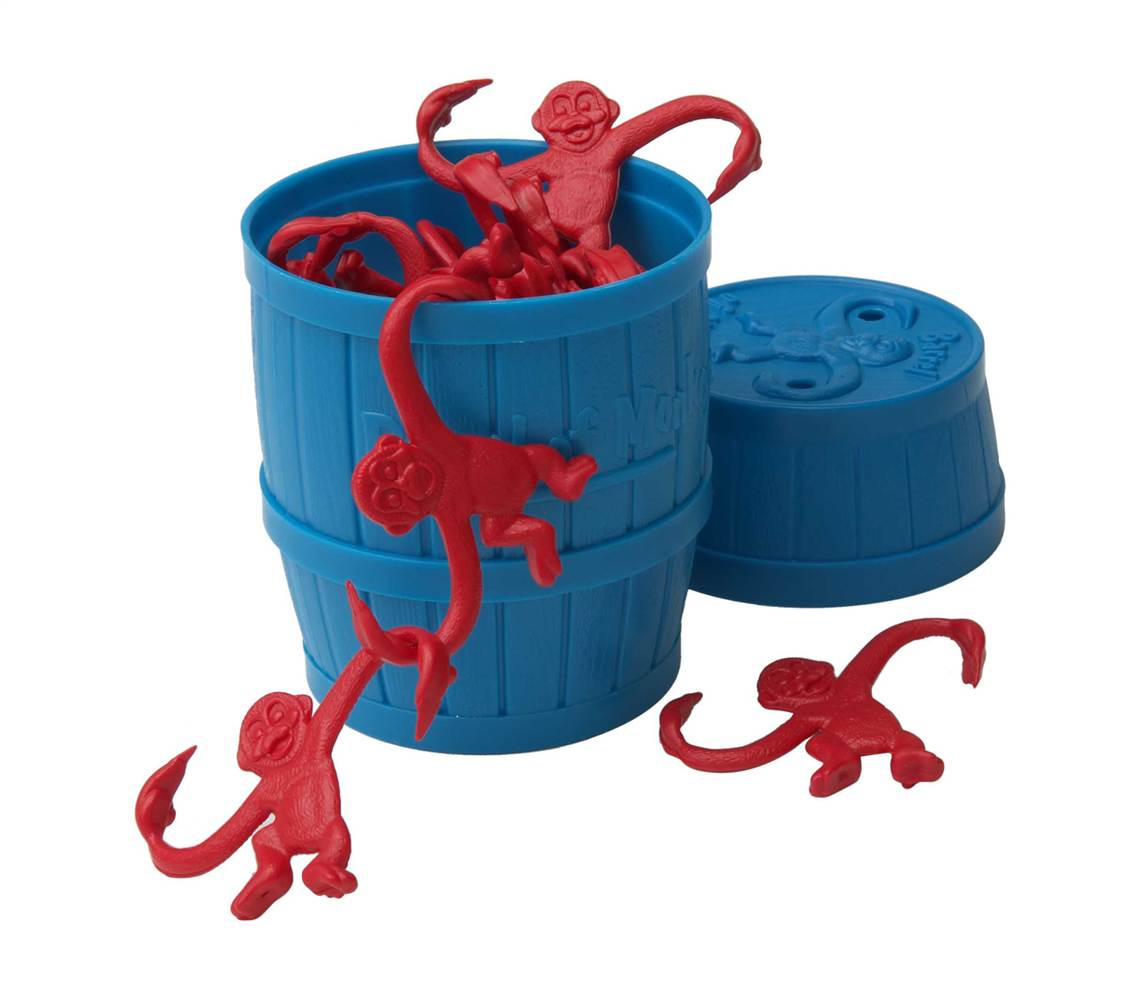
\includegraphics[width=12.1cm, height=9cm]{typescript/barrel-file/monkey-barrel}

\subsection{ Barrel File In Practice }
In the previous chapter we discussed doing something like the following:
\begin{lstlisting}
import {module} from '@ill/color-picker';
\end{lstlisting}

We are able to do this, because the nrwl nx layer on top Angular CLI, will
generate an index.tx file which will contain all imports. Anything that is
within the component, that should be exposed outside the lib, should be put
in the index.ts(barrel file).

\begin{lstlisting}[caption=index.ts]
export { IllColorPickerModule } from './src/ill-color-picker.module';
\end{lstlisting}

\subsection{ Enforcing Barrel File With Tslint }
In addition, Nrwl nx has a tslint add on called nx-enforce-module-bounderies.
\begin{lstlisting}
// tslint.json
"nx-enforce-module-boundaries": [
      true,
      {
        "allow": [],
        "depConstraints": [
          {
            "sourceTag": "*",
            "onlyDependOnLibsWithTags": [
              "*"
            ]
          }
        ]
      }
    ],
\end{lstlisting}

Adding true, will make the tslint complain whenever we are not using the barrel
import when accesing a lib file.


\section{ Typescript - Getting and Setting  }
Creating a getter and setter is a common occurance in OOP paradigm. When using
a class, Typescript offers an internal getter and setter. It is important to
note that within the Typescript documenation, a large part of the reason why
they create setters and getters, is to give a way of intercepting the setting
of a particular element. \footnote{typescriptlang.org\/docs\/handbook\/classes\.html}
For instance, let's say that you want to give people the ability for it to
error out if it doesn't actually contain one, or two strings. Doing something
like that with a setter is great.

\subsection{ Typescript - Why create a getter and setter? }
Another important point, is the syntactic sugar for two reasons.
\begin{enumerate}
  \item Getting and setting is a integral part of OOP programming. Before redux
  came around, it was literally a part of every component without a doubt.
  Having a functiin pegged with a get, or set directly before the function, helps
  specify the intent of the getter, or setter.
  \item While yes it is true, that one would be able to specifiy a function that
  will act as a setter or getter, it is syntactically, a bit awkward within an
  OOP setting. If I may:
  \begin{verbatim}
    getDinerText()
  \end{verbatim}

  \begin{verbatim}
    Diner.text
  \end{verbatim}
\end{enumerate}

So yes, can you set and get, without using the internal setter and getter that
Typescript has to offer like everything else, yes. However, the syntactic sugar
will make it seem like you are natively setting and getting. In addition,
putting emphasis on whenever an item is getted, or setted.

\subsection{ Valuable getting and setting within an ngrx/store setting }
So the question then becomes, if you are using ngrx/store within your app, for
what reason would you hvae value for getting and setting. For the most part, the
values that you have will either be set through @Input's within Angular, or
accessed through your @ngrx/store. There is one in particular very valuable
reason. That would be if within your Typescript component you have deep nested
data. Having a getter and setter within a component would be very useful. For
instance:
\begin{lstlisting}
get numberOfDocuments(): number {
  try {
    return this.userLog.user.documents.length;
  } catch (e) {
    return 0;
  }
}
\end{lstlisting}
Now we have a getter with logic, that says that if it doesn't exist, then it
will return something 0. We can then do something like the following:
\begin{verbatim}
<span> Number of Documents: {{ numberOfDocuments }} </span>
\end{verbatim}
in your html.

\maketitle{}
\section{ Typescript - Immutability }
Immutability is one of the core concepts when it comes to data. I first learnt
about it when I was introduced to Redux. However, as time progressed it was
something that I learn to integreate with all of my projects. With regards to
Typescript, it allows type annotations in the way of Immutability:
\begin{lstlisting}
export interface User {
  readonly firstName: string;
  readonly lastName: string;
}

let user: User = {
  firstName: 'Larry',
  lastName: 'Snow'
};

// This will result in a compile time error
person.firstName = 'Pam';

\end{lstlisting}

Instead this promotes using immutability. So if someone would like to turn this
data into something else, they would do something like the following:

\begin{lstlisting}
export interface NewUser extends User {
  location: string;
}
let newUser: NewUser = {
  ...user,
  location: 'New York'
};
\end{lstlisting}

\maketitle{}
\section{ Using Angular CLI in an Nx Workspace }

Now that we have created an nx workspace, let's create our app. Run
\begin{verbatim}
  ng g app angularPixelIllustrator --routing
\end{verbatim}

This will create an app called angular-pixel-illustrator\footnote{that's right
angular cli will automatically convert camel case to dash case} with routing
capabilities using the Angular CLI \footnote{If you will recall, we discussed
the Angular CLI folder/file directory in the Angular CLI Chapter}.

We can now serve\footnote{I.e. run on a server for development reasons} our app,
by running:
\begin{verbatim}
  ng serve
\end{verbatim} \footnote{It's important to note, that ng serve will open up
angularPixelIllustrator by default. As we begin to add more apps, it will make
more sense to specify specific app being opened.}


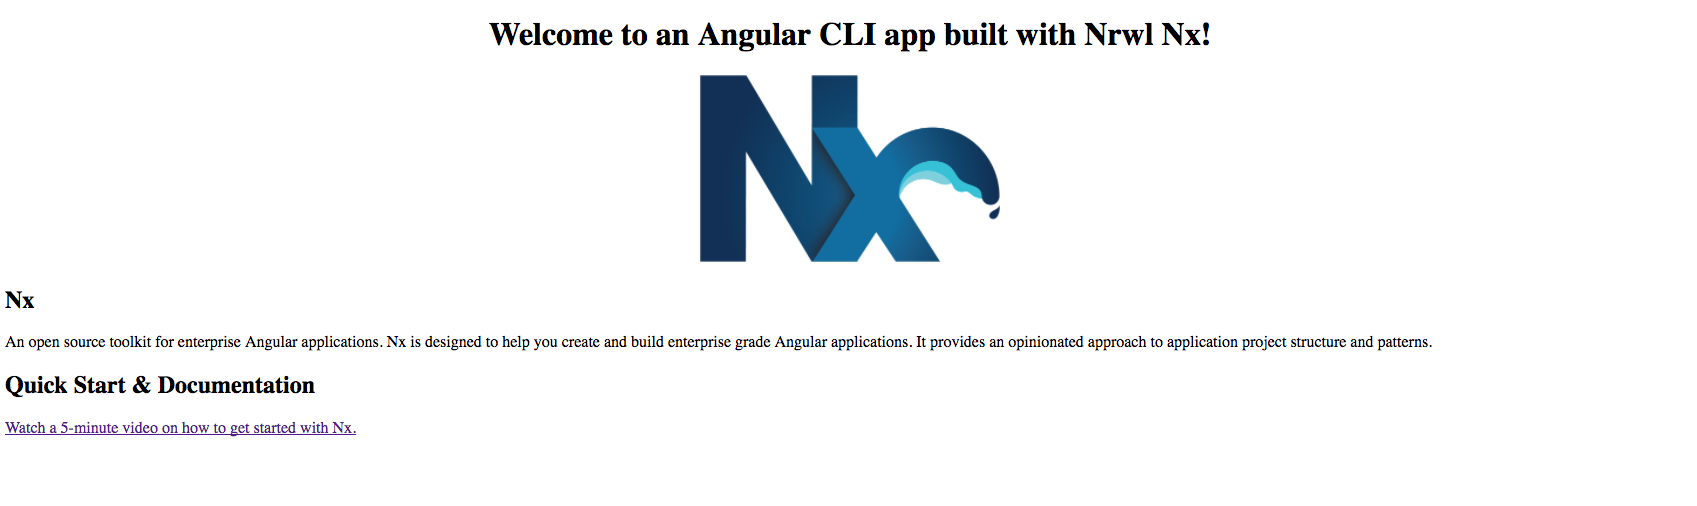
\includegraphics[width=13cm, height=9cm]{angular-cli-post-nx/angular_nx_initial_screen}

At this time, if you were to go to localhost:8080 you will see our app, is
ready to go.

Let's now create our first component. For our Pixel Illustrator, we want a form.
We will name the component chooseSize.

\subsection {Wait a Minute!}
Before we go ahead and create our component, we are going to want to tidy up
our folder architecture. The architecture we are introducing in this book is
heavily influenced by two projects. One, Nrwl, and by extension Nx. The other is
the example app, introduced in the ngrx/platform repo \footnote{It can be seen
here: https://github.com/ngrx/platform/tree/master/example-app}.

\subsubsection {Sidebar}
At the time of thiwriting there is one main area of conflict with regards to
ngrx/store v. Nx. Even though we have not experienced it yet, it makes sense to
talk about it before moving on from the cli/nx workspace chapters. Nx is very
opiniated with regards to it's folder structure. It believes everything should
be turned into it's own module, and all files related to that module should
be encapsulated inside of it. This includes (and if you are not familiar, do not
worry, we will get to it in later chaptes ) pipes, services, interfaces, guards,
and enums.

In the ngrx/example-app project, these will be split into separate folders, and
the appropriate file, will be put into that specific folder. I would imagine
that many on the ngrx/platform team agrees with nrwl/nx. I most certainly do,
and especially with state management, it makes sense for all others items to
be encapsulated into their appropiate folder. If it is something that should be
shared across app, then it should be put into it's own library. Something that
we will discuss moving forward.

\subsection {Phew, sidebar over, moving on}

The above being said, whenever we create a component, we are going to want to
encapsulate it, into a local module. That way we can add state, pipes, services,
you name it, and it will all be encapsulated in that component folder.

In order to create our module we run the following angular cli command:

\begin{verbatim}
  ng g module choose-size
\end{verbatim} \footnote{Once again we have the liberty with not having to
specify the app name}

Then, in order to create our component:
\begin{verbatim}
  ng g component choose-size
\end{verbatim}
The following five files have been created (using git diff --cached)
\begin{lstlisting}[breaklines]
new file:   apps/angular-pixel-illustrator/src/app/choose-size/choose-size.component.css
new file:   apps/angular-pixel-illustrator/src/app/choose-size/choose-size.component.html
new file:   apps/angular-pixel-illustrator/src/app/choose-size/choose-size.component.spec.ts
new file:   apps/angular-pixel-illustrator/src/app/choose-size/choose-size.component.ts
new file:   apps/angular-pixel-illustrator/src/app/choose-size/choose-size.module.ts
\end{lstlisting}


\section{ Format all the things }

In a Nrwl setting, we have a format npm script that is available to us by default.
It is called:

\begin{verbatim}
  nx format write
\end{verbatim}

This will call, a .prettier file that has been created by the nx workspace
command. Prettier is similar to to the CLI to the extent that there is a lot
that is happening behind the scenes. In short, it will automatically format files
for you, to it's liking. It's like a pro-active linter, that will format code
for you.

Two architectural talking points, with regards to prettier:
\begin{enumerate}
  \item You will have to format your tslint, so that it does not compete with prettier.
  \item You are going to want to hook up prettier with your IDE, so prettier
  can go to work without having to run it in your terminal.
\end{enumerate}

Note: We are going to have to create a way that we can update the prettier file
automatically.

\subsection{ How to add prettier to Webstorm }
As we mentioned in a previous chapter, Webstorm is our IDE of choice. VIM users
and Atom users, I completely respect your decision, and feel free to code in
that capacity. However, my experience working with large teams, is  that Webstorm
has a lot to offer outside of the box. For the non power user, it will offer
all of those benefits. Ok, great, the following is how to add prettier to Webstorm
with a screenshot!

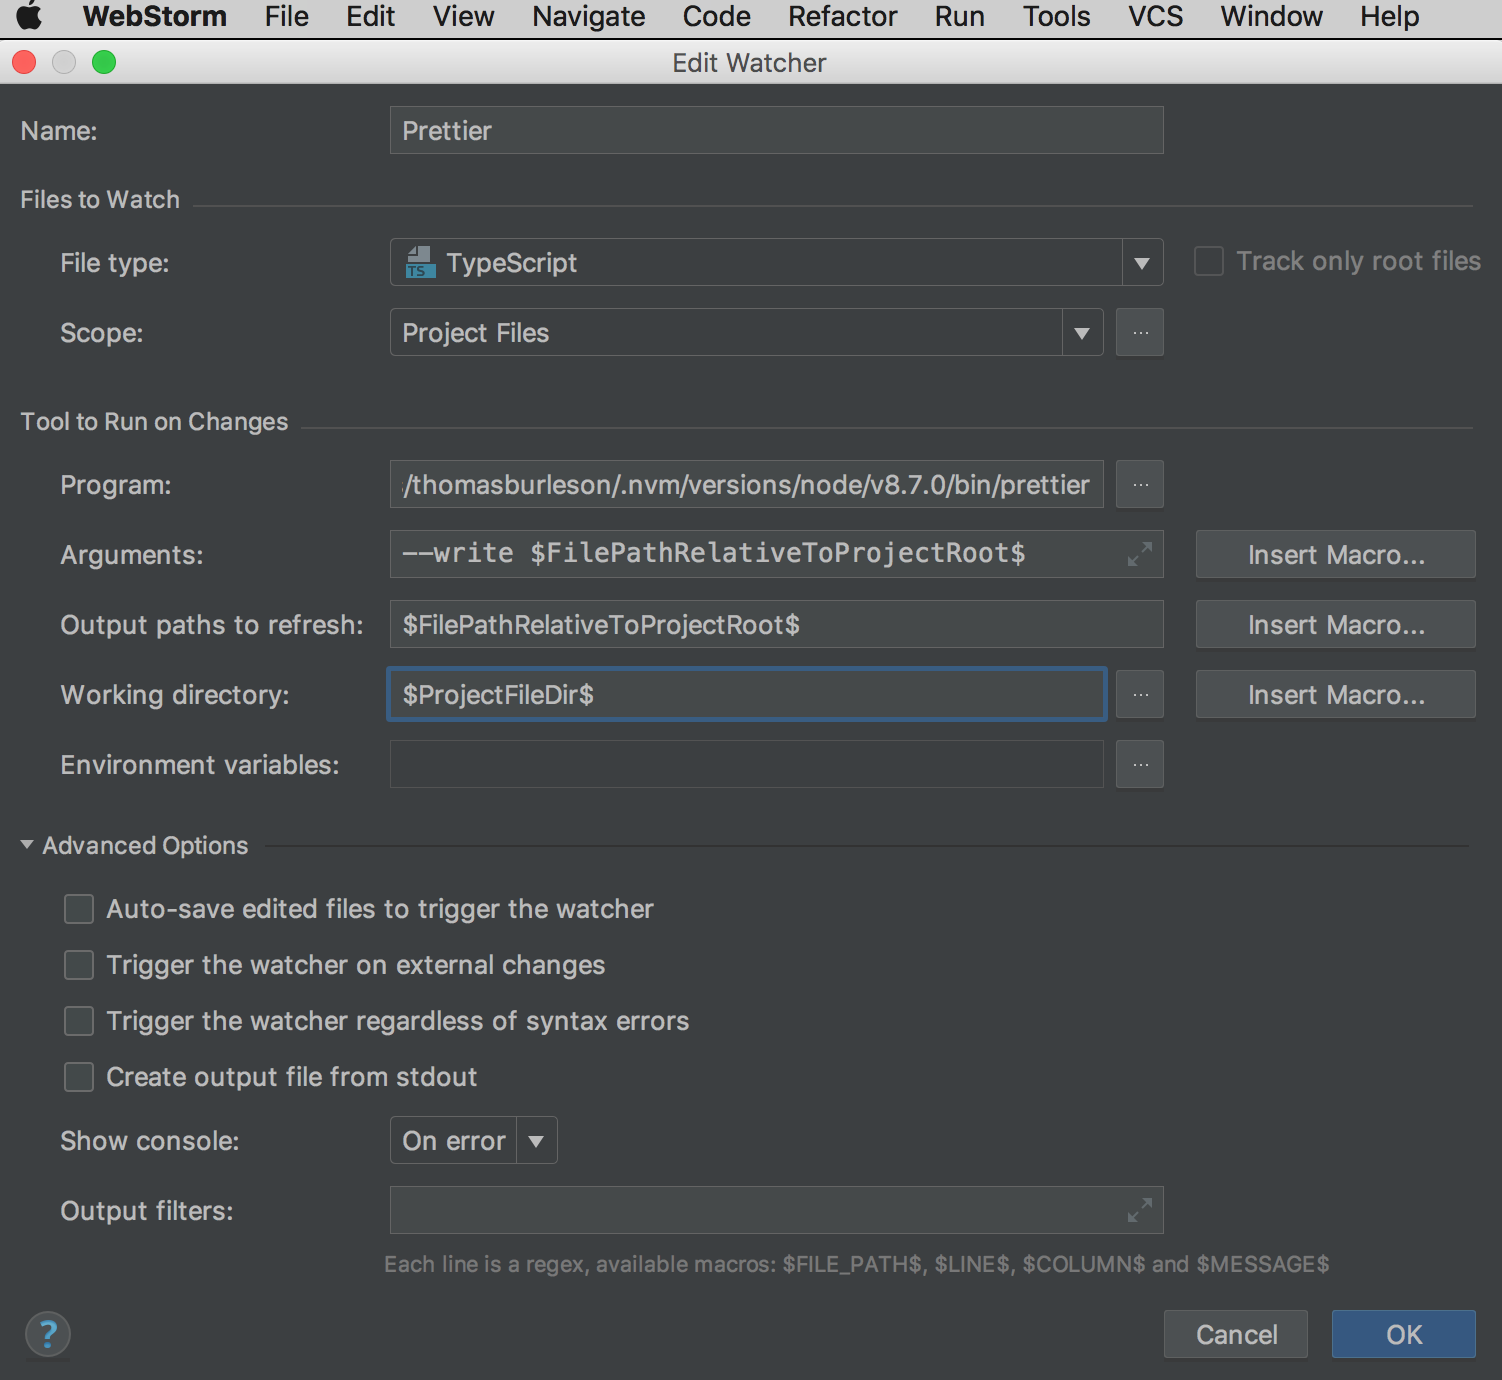
\includegraphics[scale=0.5]{format-all-the-things/prettier-file-watcher-webstorm}

\maketitle{}
\section{ Lint all the Things }

\subsection{ Lint all the Things }

Linting is incredibly important. Think of it this way. Someone's favorite food
item might be brocolli, another person's favorite food item, might be steak.
Now the two might work well together(on a number of levels, mmm hungry), but
forcing one person to adopt the other food item as their favorite, is unjust!

Ok, bad example, but the concept is the same. Things such as how many spaces per
indentation, double quotes vs. single quotes, trailing commas, empty interfaces,
these are all important points. To be honest, I've only found my peers arguing
on more minute points, such as double vs. single quotes, and how many spaces
per indentation. Therefore, linting allows:
\begin{enumerate}
  \item Agreement on code formatting rules.
  \item Automated way of keeping track of things that need to be changed.
  \item Self documentation through cli, on what needs to be changed.
\end{enumerate}

Another important point, is that we would ideally like a formatter, that
automatically formats these things for us. So, from an architectural perspective
when we are looking for a linter, we are also looking for a formatter to go along
with it.

\subsection{ What are we trying to lint? }
We are trying to lint HTML, SASS, and Typescipt. Angular CLI, offers Tslint out
of the box. 


\section{ Linting Sass }

As we mentioned in the previous chapter, there is a greate matter of importance
when it comes to linting. In particular when it comes to sass, the Angular CLI,
nor the Nrwl Nx cli will offer sass linting out of the box. In particular,
we will be choosing the package sass-lint.

\subsection{Installing Sass Lint}
\begin{verbatim}
  npm install sass-lint --save-dev
\end{verbatim}

\subsection{Adding a Lint Config File}
For sass-lint, it will hook into by default a file that is in the root of
folder called .sass-lint.yml. It's quite long, and you can see the rest of the
file in the actual github repo. However, you would create a sass-lint.yml file.
\begin{verbatim}
  touch sass-lint.yml
\end{verbatim}
Inside of the sass-lint.yml file, it will look something like this:
\begin{lstlisting}
options:
  formatter: stylish
files:
  include:
    - '{apps,libs}/**/*.scss'
  ignore:
    - 'libs/font-awesome/**/*.scss'
rules:
  # Extends
  extends-before-mixins: 1
  extends-before-declarations: 1
  placeholder-in-extend: 1

  # Mixins
  mixins-before-declarations: 1

  # Line Spacing
  one-declaration-per-line: 1
  empty-line-between-blocks: 1
  single-line-per-selector: 1

  # Disallows
  no-attribute-selectors: 0
  no-color-hex: 0
  no-color-keywords: 1
  no-color-literals: 1
  no-combinators: 0
  no-css-comments: 1
  no-debug: 1
\end{lstlisting}

The list for what sass-lint disallows goes on and on. Some of the linting rules
I really like is no color words, empty line between blocks, bem-depth, for
starters. From an architects perspective, and from a developers perspective, it
has made the code review process much easier. When this linting process is
combined with the functional sass paradigms we will mention, it becomes
self managing architecture for styling. Let me say that again, SELF MANAGING. I
thought that might be worth repeating.

\subsection{Adding an NPM Script in your package.json}
\begin{verbatim}
  "lint-scss": "sass-lint -v -q",
\end{verbatim}

\subsection{The Final Touch}

Adding the sass-lint npm script as part of your CI/CD architecture is what
really brings it all together. This is twofold of course. One so that when you
make a pr for your Github repo, it will check to make sure there are no Sass
linting errors. In addition, when pr is actually merged, pipeline runs as well,
to make sure there are no errors.

\maketitle{}
\section{ Linting HTML }

Linting html is not as mature as it is with regards to Sass and Javscript in my
opinion. Howvever, that makes sense as html is essentially strucutred xml that
is used within the context of a web app.

That being said, once again, there is no linter that is offered out of the box
through the Angular CLI, or Nrwl Nx either. It is, however, beneficial.

\mybox{
\subsection{ Side Bar }
Why not use something like Pug(once called Jade) for html templating. The main
benefit of something like Pug I have found is that it tells me where the html
begins and ends. In a complex html element, where there are many levels of
nesting this can be beneficial. However, in a templating engines, there tends to
be many quirks, in particular when it comes to using various frameworks. I have
rarely been on a team where after selling Pug, engineers have been enthusiastic
in using it.
}

\subsection{Why We Chose HTML Hint}
The honest truth is that the landscape for html hasn't drastically changed at
it's core level over the past couple of years. Of course, if there was a more
mature linter, the linter would complain that the engineer should use certain
html element as opposed to another. That being said, we have found html hint
to be the most robust html linter, even though development has been lack luster
over the past couple of years.

\subsection{Installing HTML Hint}
\begin{verbatim}
  npm install htmlhint --save-dev
\end{verbatim}

\subsection{Create an .htmlhintrc config file}
In the root of your app, create an .htmlhintrc file. The .htmlhintrc is set up
to be the default config name for html hint. A sample config for html hint will
just be a simple JSON object containing key values. For instance:
\begin{lstlisting}
{
  "attr-value-double-quotes": true,
  "src-not-empty": true,
  "alt-require": true,
}
\end{lstlisting}

\subsection{Adding an NPM Script in your package.json}
\begin{verbatim}
  "lint-html": "htmlhint --rulesdir './rules/' '{apps,libs}/**/*.html'",
\end{verbatim}

\subsection{Adding a Rules Directory for html hint}
You will notice that inside of our html hint command, we have created a rules
directory. We are doing this so that we can potentially create our own sample
html hint rule.

\subsection{What a Sample Rule Looks Like}
In the root of your directory, create a rules directory. Inside of that
directory, let's create some sample logic:
\begin{lstlisting}
module.exports = function(HTMLHint) {
  HTMLHint.addRule({
    id: 'attr-space',
    description: 'Attributes cannot have useless whitespace between "=" and attribute name or attribute value.',
    init: function(parser, reporter) {
      var self = this;

      function handleTagStart(event) {
        var col = event.col + event.tagName.length + 1;

        event.attrs
          .filter(function(attr) {
            return attr.value;
          })
          .forEach(function(attr) {
            var rawAttr = attr.raw;
            var indexOfEqualSign = rawAttr.indexOf('=');

            if (rawAttr.charAt(indexOfEqualSign - 1) === ' ') {
              reporter.warn('Space between attribute name and "="', event.line, col + attr.index + indexOfEqualSign - 1, self, attr.raw);
            }

            if (rawAttr.charAt(indexOfEqualSign + 1) === ' ') {
              reporter.warn('Space between "=" and attribute value', event.line, col + attr.index + indexOfEqualSign + 1, self, attr.raw);
            }
          });
      }

      parser.addListener('tagstart', handleTagStart);
    }
  });
};
\end{lstlisting}

The above allows for a robust html lint archticture, with the ability to add
more rules if need be.

\maketitle{}
\section{ Material Design }

I was debating writing this chapter. The reason primarily being, that depending
on the size of your company, you might up end writing your own design system. I
completely understand that, and it makes sense if you are a B2C
\footnote{Business to Consumer} enterprise.

However, I truly do not understand why a company using angular 5, or 6, would
not want to use material design. It is the most robust design framework that
exists within open source. In addition, the documentation for Angular components
is next to none. I personally have been in companies where they had a business
to business application and they decided not to use material design.

I really do not understand the reason for doing this. They could have saved
loads of resources not having to design and implement their own components. It
is out of the vast amount of use cases that I see Material Design being valuable,
that I have decided to go ahead and write about it.

\subsection{ Material Design - Talking to UX/UI }
This section right here, is perhaps why I like Material Design the most. Material
Design has documentation for how the UX should work. It also has an Angular
component library with demos, that I can show off to UX and show them, this is
how it works by default. It addition, theming for Material Design, is very easy.

Putting your own company specific spin on it, boils down to the following:
\begin{enumerate}
  \item Colors
  \item Font
  \item Spacing(Margin + Padding)
  \item Icons(not that this is anything particular)
  \item Buttons
\end{enumerate}

The above would be it for starters. As your designs go on, you will have components
that you will end up overridig.

\subsection{ Material Design - Create your own Confluence Doc }

It is important when working with UX/UI to document discrepencies. For
inspiraiton look at the \href{material design docs}{https://material.io/guidelines/components/sliders.html}.
The idea is to have a central place where UX can create Confluence doc
describing the differences they have made from DLS.

Engineers will generally have to be the one to begin the Confluence doc. From a
matter of ownership, engineering has a stronger discipline of documentation and
organization. Engineers should look to take ownership of the confluence doc.

\subsection{ Material Design - Use Invision }
It's interesting, because someone might not think of tooling as something which
is a part of engineering architecture. However, with regards to finding
discrepencies in DLS(Design Language System), Invision is integral. It will
make creating comments on particular components as something which will be fluid.

\subsection{ Material Design - Push Back }
The following will be worth alot of time for many different people within your
organization. Make sure that your component does not deviate from Material
Design. In addition, look into whether, or not it is pre-described for you to
go ahead, and create your own components. However, I can assure you designers,
product/business, and engineers will all be happy when you go with the default
components when possible. When building a product, unless it is beyond the MVP
go with what is available for you by default. 

\maketitle{}
\section{ Design Language System }

Creating a design language system is imperative to any architecture. Within
Angular the Full Gamut, we are going to assume that you are using Material
Design as your DLS. Reason as we discussed before, is that it is the most robust
library for creating Angular components. However, there are particulars of
Angular that one is going to want to modify. This is where having a light
design language system coming in can be very important.

\subsection{ Identifying Key Points of DLS }
The following are the 10 points that are a part of DLS:

\begin{enumerate}
  \item Colors
  \item Styles
  \item Icons
  \item Grid and Spacing
  \item Typography
  \item Buttons
  \item Form Controls
  \item Navigation
  \item Cards and Portlets
  \item Data Tables
\end{enumerate}

These are arguably the 10 parts of any material application that will be used
the most.

\subsection{ Identifying Proper Architecture }
With regards to overriding material design, is the part where architecture kicks
in. This is a very important part of the application and I will go through one
by one, the parts of the application that have similar architecture with regards
to overrides.

\subsubsection{ Colors }
Material design has the ability to be overriden in a sass file. It is important
to note, that the material theme allows for overrides using Sass Variables. So,
one would do something like this:
\begin{lstlisting}
@import 'src/styles/themes/blue-orange';
@import 'src/styles/material-overrides/material-overrides';
\end{lstlisting}

Doing something like the following:
\begin{lstlisting}
$gray-50: #fafafa;
$gray-200: #dbe1ea;
$gray-300: #e0e0e0;
$gray-400: #cccccc;
$gray-500: #bdbdbd;
$gray-600: #9b9b9b;
$gray-700: #757575;
$gray-800: #444444;
$gray-900: #212121;
\end{lstlisting}

Now the colors you have are specific to your app.

\subsubsection{ Grid and Spacing }
This one etc.

\maketitle{}
\section{ Icons }

I would like to dedicate a quick chapter to icons simply because I have never
come across an application that has not used icons.

\subsection{ Font Awesome }
However, in short, using font-awesomein the largest icon library, and the pro
version is relatively cheap. In addition, there are many particulars with icons
that they solve, making sure that they look good on different devices. So, in
short I would like to reccomend font-awesome, it is the best architectural
decision you can make when it comes to fonts.

\subsection{ When Font Awesome is Not an Option }
However, there are times within one's app wherein Font Awesome is not an option.
At that time, it is appropriate to roll up one's sleeves and put on the
architectural hat for icons. It is important to keep the following in mind.

\maketitle{}
\section{ Sass Error Reporting }

\subsection{ When to use Sass Error Reporting }
One should use Sass Error reporting if it is a core style. It is a core style if
it is used in more than one page, as a foundational piece of styling, non
unique to specific component.

\subsubsection{ What We Are Looking For With Using Sass Functions }
\begin{enumerate}
  \item No values other than these are used
  \item When a Pr comes our way, and we say to use the above, we have a function which is self documenting.
  \item Have a UI of sorts that also trains developers on how the internal of
  the DLS works, so that they should be aware if anything is wrong.
\end{enumerate}

\begin{lstlisting}
// Gutter variables, for padding + margin
// function to take in multiplier(8), which must emit of one of values within mc-space-amounts
@function mc-space-multiplier($n) {
  $ill-space-amounts: (0, 4, 8, 16, 24, 32, 40, 48, 56, 64);
  $ill-space-multiplier: 8;

  @if(index($mc-space-amounts, ($n * $mc-space-multiplier))) {
    @return #{$n * $mc-space-multiplier}px;
  }
  @else {
    @error "Must contain one of the following numbers: #{$mc-space-amounts}.";
  }
}
\end{lstlisting}

In this particular situation this helps, so that if the input passed to the
multiplier is not a number, it will complain. In addition, if the result is not
one of the multipliers, it will complain as well. So for instance, if the number
passed in, is 1.5, it will cause the function to error out, being that there is
no number 12, that is one of the ill space amounts.

\maketitle{}
\section{ Sass Unit Testing }

\subsection{ When Does Sass Unit Testing Make Sense? }
One of the concerns with any architecture, is over engineering. With regards to
unit testing Sass, to what extent should one unit test? Should it be for every
class, for every function, any core class used within a framework.

Being that we are going to be creating sass functions for our core theming, it
would make sense to unit test them as well. If they are going to be use in 10,
or more places per each app, then we would like to make sure, that they are
indeed working in the fashion that they should be.

\maketitle{}
\section{ Creating Code Owners }

As we have discussed previously, Github is our preferred client for pull
requests. As the team grows larger it becomes imperative, that default code
reviewers are setup. Creating a \codeowners{} file is the easiest way to do this.

\section{ What is a \codeowners{} file? }
A \codeowners{} file is a config file, used with Github, that will allow you to
specify which github users are considered as \codeowners{} for a specific project.
In addition, it will allow you to target \codeowners{} for a specific file type.
So just to go a bit more in detail, let's say you have a dynamic team, and a
dynamic codebase. Part of the team develops in Python, and part of the team
develops in Javascript. You would be able to set \codeowners{} specifically for
javascript, so that if only js files have been affected, only these specific
\codeowners{} should be brought up.

\section{ How to create a \codeowners{} file? }
There are two places wherein you can create a \codeowners{} file. One would be
in the root of your app. The other would be in a .github folder in the root of
your repo. We recommend the .github folder, as we will also be creating webhooks
within our repo. So:
\begin{verbatim}
  mkdir .github; cd .github; touch \codeowners{}
\end{verbatim}
When you make a pull request within your github app, github will automatically
pick up on this file.

\maketitle{}
\section{ Code Reviews }
Code reviews are a very intuitive process. It can potentially be looked at as
something that I would do. If the pull request isn't looking at the code the
same way I would, then I should comment. However, it's the part of commenting
and accepting criticism, that makes this is entire process very tricky.

\subsection{ Code Reviews - The Golden Rule }
There are multiple ways of doing something. If the code reviewer leaves a
comment for doing something in an alternate way, and the person recieving the
code resists, then the code reviewer has no right to insist on her/his way. It
is then important, however, from that point onwards, that the team agrees on a
convention.

\mybox{\subsection{Story Time}
  The following is a great example of how this golden rule can manifest in real
  life. Once upon a time, my team was working on a component, wherein every tab
  was to be in uppercase. The person submitting the code felt that explicitly
  typing out every word in uppercase: NAME, STATUS, TIME; Made more sense. I
  expressed that adding a css class with text-transform: uppercase;
  would make more sense. The pr submitter expressed that they felt explicitly
  typing out everything made more sense. I mentioned that ok, I can see your
  point of view, and I will remove my comment.

  The truth is that if this was a B2C\footnote{Business to Consumer}
  application, then I would have been adament about my approach. However, this
  was a B2B\footnote{Business to Business} application, and allowing this person
  to code the way they feel comfortable and be happy, because life really is too
  short, is ultimately what is important.
}

\subsection{Setting Conventions}
Another important part of the code review process is to set conventions. In my
humble opinion, the reason conflict happens with regards to code, is due to
uncertainty. When there are conventions set up before work on code happens it is
to point to code guidelines and say this is what we do. In addition, somone has
the ability to challenge code guidelines, and it is more challenging code
guidelines. This allows those involved in discussion to save face.

\subsection{ A Time to Learn }
It is also very important for others to learn. It is a way for me as the code
reviewer to ask what a certain piece of code does. A good convention is that if
it is something new that you haven't done before, then you can ask about it
and learn about it. This is one of those points that is obvious yet it is passed
on more than most.

\subsection{ A Time to Mentor }
It is also a time to setup \codeowners{} across the app, and specifically make
junior developers code owners. 

\maketitle{}
\section{ Github Wiki }


\section{ Github Board }

The github board, for open source projects is used in a task management
capacity. In an enterprise setting, it can be used to track the one thing
that can't be tracked through JIRA, app considerations.

For instance, let's say you would like to migrate your app to the latest version
of Angular. You would create a board called "Tech Concerns". You would then go
ahead and create a widget for Upgrade Angular. Everyone on your team would then
know that you have certain things that you would like to progress in tech.
This can be used for other items as well, such as change directory structure to
use mono repo, or integrate E2E tests within app.

\maketitle{}
\section{ Smart Vs Dumb Components }

In any UI framework

\maketitle{}
\section{ Dialogs }

There are certain components that are expected in any architecture. Dialogs are
one of those components. However, their architecture can be so complex, that it
is very important to come up with a strategy that works with state management.
This architecture was originally adopted from Thomas Burleson who I have a
tremendous amount of respect for.

A couple of issues that dialogs have, is that they are:
\begin{enumerate}
  \item Defined in Templates
  \item Created at App Startup
  \item Managed in UI Components
  \item They complicate UI Components
    \begin{enumerate}
      \item Open, close, cancel
      \item Services
      \item Store Actions
      \item Pending State
    \end{enumerate}
  \item Dialogs may interupt NgRx Flows
\end{enumerate}

\subsection{ Centralizing Dialogs + Best Practices}
As with the rest of our architecture, we are trying to centralize the way we
use our components. Therefore, the following are dialogs best practices:
Section 1
\begin{enumerate}
  \item Use @angular/material Dialogs
  \item Use Dialog Service to open and and manage custom dialog components
  \item Use Dialog configurations to customize dialog instance
\end{enumerate}
\begin{enumerate}
  \item Use Ngrx Effects to Manage Dialogs
  \item Inject Store/Facade into Dialog Components
\end{enumerate}

\begin{enumerate}
  \item Use Ngrx Dialog Effects
  \item Disconnect Dialog from Feature Effects
\end{enumerate}

\maketitle{}
\section{ Dependency Graph }

A dependency graph is a very simple way of seeing which components are
dependent on which components. It goes hand in hand with a parent and child
component architecture.

\maketitle{}
\section{ Containers, Routing + Ngrx/router }

We now have a choose-size component, as well as a choose-size module.
The dynamics of our app, is that there will only be two parent pages. One will
be the choose-size page. The other will be the draw page. When a user goes to
the page for the first time, they will see the choose-size page. Therefore we
are going to add two routes in our app.

In our app.module.ts, we will use the existing RouterModule that has been
created by Nx, and include it in our RouterModule:

\begin{verbatim}
  // Inside imports add
   RouterModule.forRoot([
    {
      path: '',
      redirectTo: 'choose-size',
      pathMatch: 'full'
    },
    {
      path: 'choose-size',
      component: ChooseSizeComponent
    }
\end{verbatim}

\marginpar{git commit -m 'Add a routes to the RouterModule, for the choose-size page.'}

Now that we have redirected the default homepage to re-direct to the
choose-size page, let's try it out. Open up http://localhost:4200, and your page
should navigate to the choose-size page, with the text, "Choose Size Works",
towards the bottom of the page.

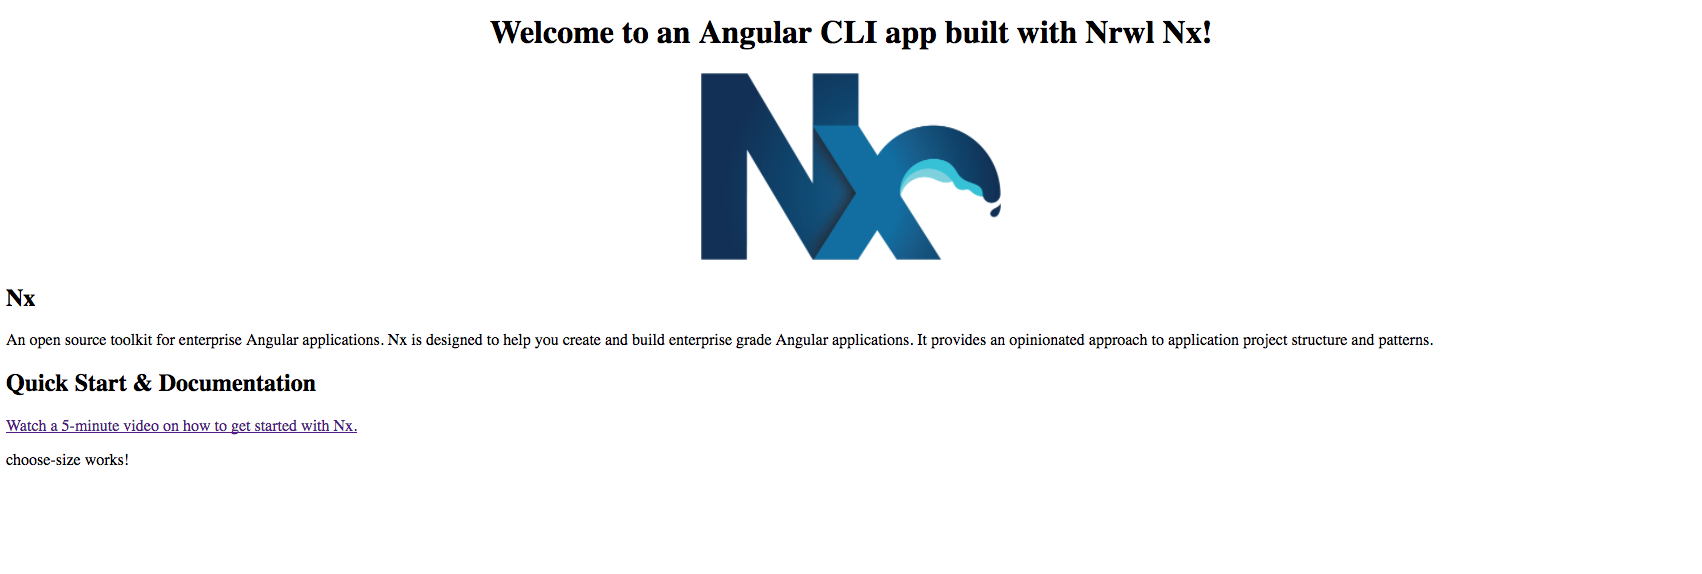
\includegraphics[width=13cm, height=9cm]{routing/containers-and-routing/choose-size-screenshot}

\subsection{ ngrx/router-store }

Before we move any further with regards to angular routes, let's discuss
ngrx/router. In short, ngrx/router exists so that the route can be in the store
as well. By default ngrx/router will dispatch a ROUTER\_NAVIGATION action
\footnote{We'll discuss this a bit more when we get to the chapter on ngrx/store},
when a navigation route get's called. This will enable time traveling with
regards to routes.

\subsection{ Why use ngrx/router-store }

Ngrx/router-store can be advantageous in two regards. One, it adheres to the
principle of there being a single state of truth \footnote{https://redux.js.org/docs/introduction/ThreePrinciples.html\#single-source-of-truth}.
Two, it helps applications with regards to breadcrumbs, and adding filters to the
url. If one wanted to follow an architecture, where the route contains the current
state of the application(filters, inputs etc.) router-store definitely make's it
very easy to do so.

\subsection{ Adding ngrx/router-store to our app }

In order to add ngrx/router-store to our app, run:
\begin{verbatim}
  npm install @ngrx/router-store --save
\end{verbatim}

In addition, we will be adding the route to our store for the first time, so we
will be needing ngrx/store. Please run \footnote{This will also install ngrx/store-devtools + ngrx/effects}:
\begin{verbatim}
  npm install @ngrx/store --save
\end{verbatim}

In our app.module.ts we will be adding the following:
\begin{lstlisting}[caption=My Javascript Example]
  + import { StoreModule } from '@ngrx/store';
  + import { StoreRouterConnectingModule, routerReducer } from '@ngrx/router-store';
  + import { StoreDevtoolsModule } from '@ngrx/store-devtools';
  // inside of imports
  + StoreModule.forRoot({
  +    router: routerReducer
  + }),
  + StoreRouterConnectingModule.forRoot({
  +   stateKey: 'router'
  + });
  + StoreDevtoolsModule.instrument({
  +    maxAge: 5
  + }),
\end{lstlisting}

\subsubsection{ Side note when using devtools with ngrx/router-store }

One final note when using ngrx/store router-store with devtools. The
RouteStateSnapshot is a very large object, containing large amounts of data. I've
run across performance issues, it is therefore reccomend setting up a
custom router state serializer
\footnote{https://github.com/ngrx/platform/blob/master/docs/router-store/api.md\#custom-router-state-serializer}.
The idea is that the user provides the specific items one wants from the route.
This allows for maybe 3 key/values to appear, instead of a 1000+. For the sake of
brevity, we will not include the technical steps here. However, the code for doing
so can be found in the github branch equivalent.

Now that we have our first route set up, as well as ngrx/router-store, let's proceed
to building a component.


\section{ Lazy Loading Routes }
One of the more initally overlook routing architectures when it comes to routing
is lazy loading. That would simply mean that a module is only loaded once
the page goes to a specific route. This will cause large initial loading times
if all of the pages are initially bundled into the root app.

An example of a lazy route is as follows:
\begin{lstlisting}
{
  path: 'customers',
  loadChildren: 'lib/users/users.module#UsersModule'
}
\end{lstlisting}

As mentioned in the actual docs:
\mybox{ The router will use registered NgModuleFactoryLoader to fetch an
NgModule associated with 'team'. Then it will extract the set of routes defined
in that NgModule, and will transparently add those routes to the main
configuration.}

\subsection{Adding a tsconfig.app.json config}
Therefore, we need to set up a config inside the main tsconfig.app.json in the
include imports:
\begin{verbatim}
  "include": [
    "**/*.ts",
    "../../../libs/users/users/index.ts"
  ],
\end{verbatim}

\subsection{Adding forChild inside of Actual Route}
\begin{lstlisting}
RouterModule.forChild([
  { path: '', component: UserComponent },
]),
\end{lstlisting}

The above is the cookie cutter process involved with create a component with a
lazy route. It is architecture that is worth implementing early on in the app.
Especially being some future components such as side navigations and modals
might be complicated.

\section{ Services }
\maketitle{}

Services in Angular can be a very confusing topic. I know that for myself it's
been very confusing. A very common core concept in programming is DRY. That is
do not repeat yourself. If there is an option to do something once, and re-use
it throughout one's application, then that is what someone should do. Services
very much so fill in this gap. That is, any functionality that is contained
within a component should be put into a service. That service now serves two
purposes:
\begin{enumerate}
  \item Keeps the component logic-less. Any logic, is now transferred over to
  the service.
  \item It potentially allows the service to be re-usable.
\end{enumerate}

The above is the base role of a service. It is what is a result of the common
sense principle of DRY.

\subsection{ Where Services Get Complicated }
At this point, services start to get complicated. The following is a great
example. Let's say we have an overview page. Any logic on the overview page is
going to be unique to the overview page, as it's logic is unique. So we create
service that is unique for the overview page. Now that isn't neccesarily dry is
it? I mean, the component could have very much so done what the service is doing.
In addition, when it comes to unit testing, it probably would be easier to keep
it all within the component.

There are other dillemas, such as what happens when we are using a service to
fetch data. What about a service that is used for graphics? What about a
service that we use for handling errors? They end up becoming abstracted to the
point, where it is very much so more beyond being DRY. It is pure logic, that
is really independent of any component. It beckons a more proper definition.

\subsection{ Services - Creating a more Robust Definition }
Service is a broad category encompassing any value, function,
or feature that an app needs. \footnote{https://angular.io/guide/architecture-services}
Services fill any gaps left by any other part of any application. In a perfect
world, services will solely interact with data, and should be doing so 80\% of
the time. The other time, should relate to how the data comes back. The question
then is, what about the other 20\% of the time. At this point, it's important
to go through other areas of Angular. 

\section{ Directives }
\maketitle{}

Assuming you are already familiar with Directives, at first glance having
components and directives can seem a bit superfluous. They both seem to do the
same thing. However, in summary, the following is a very clear cut definition
between directives and components.
\mybox{
 A @Component requires a DOM whereas a @Directive does not
}

\subsection{ What Definition Translates To }
What this definition translates to is that if there is something that translates
as a piece of functionality that you woul consider as an add-on, make that a
directive. Something that would be considered as it's own self contained UI
element, it should be considered as a component.

\subsubsection{A Great Example}
A great example of this, is adding drag and drop functionality to a component.
That in it's self is not component worthy. However, adding a dropzone directive
to the element, would make any potential component drag and droppable worthy.
A great example of a component, would be a data table. A large part of it's
functionality is strickly tied to actual UI element.

\mybox{
  A side note with regards to our architecture, directives will be very used. If
  you find yourself writing, with what feels like too many components, don't
  worry, it's to be expected.
}

\chapter{ Pipes }


Angular offers the ability to use something called a pipe out of the box. The
idea behind a pipe is to get data, transform it, and show new transformed data
to users. It is a very common task, and Angular, rightfully so, decided to
include it in it's framework. The easiest way to think about it, is a way
to put a function in your html template!

A pipe might look something like this:

\begin{lstlisting}
import { Component } from '@angular/core';

@Component({
  selector: 'app-data-table',
  templateUrl: './data-table.component.html',
  styleUrls: [./data-table.component.scss],
})
export class HeroBirthdayComponent {
  transaction = new Date(1988, 3, 15); // April 15, 1988
}
\end{lstlisting}

begin{lstlisting}
<!--data-table.html-->
<Div>Data of transaction {{ transaction | date }}</p>
end{lstlisting}

The above would display:
\begin{verbatim}
April 15, 1988
\end{verbatim}

The pipe in this instance, will transform transaction, from a Date object, and
transform it to a readable date.

\section{ The Uniqueness of Pipe }
The unique part about an Angular pipe, is that it is something that will be
defined as a function, but actually be in your html. Any classic way of
thinking of a function can similarly be applied to a pipe.

\section{Chaining Pipes}
If you want, you can chain multiple pipes together, similar to function
composition, to allow for multiple effects on your html.

\begin{lstlisting}
The chained transaction date is:
{{ transaction | date | uppercase}}
\end{lstlisting}

Would display
\begin{verbatim}
APRIL 15, 1988
\end{verbatim}

Chaining pipes, walla!

\section{Parameters for Pipes}
Pipes also take parameters, similar to how functions take parameters. For
instance, if we want to add a parameter to the default Angular pipe. For
instance, let's say that we wanted to show the day of the week, in addition to
actual week we can provide the pipe the following param:

\begin{lstlisting}
The chained + formatted transaction date is:
{{ transaction | date: "full" | uppercase}}
\end{lstlisting}

Having such dates in one's application obviously makes it very easy to go ahead
and transform data throughout one's app. Here we are also chaining pipes, so
that the transformed data that comes back in addition to being transformed, is
also capitalized.

\section{ Dis-chapter of Angular Built in Pipes }
I think it's important to show that Angular actually has a relatively limited
amount of built in pipes:
\begin{center}
\begin{tabular}{ c c c }
 AsyncPipe & CurrencyPipe & DatePipe \\
 DecimalPipe & i18nPluralPipe & i18nSelectPipe \\
 JsonPipe & KeyValuePipe & LowerCasePipe \\
 PercentPipe & SlicePipe & TitleCasePipe \\
 UpperCasePipe
\end{tabular}
\end{center}

The reason behind it, is that truly the beauty behind pipes, is that you have
the ability to create your own. The community, for instance, has created a vast
amount of pipes beyond that of the built in one's Angular has created.

\subsection{ Understanding Angular's Change Detection }
This is a good time to interject and get into the nitty gritty of angular's
change detection. As we discussed in the earlier chapter on change-detection,
change detection in Angular works from the top down. That is, if a specific set
of data changes within a component, then the entire component will update as a
result of new data. Angular pipes, however, change how that it is done, by
changing content directly on the object, and only updating that one specific
part. By using pipes, it allows one's component to be more performant.

\section{ When to Use Pipes }
Pipes cover alot of ground. Within our architecture, one of the pipes that will
be used more so that others is the async pipe. However, now is not the place
to put that here. What is important, is that pipes can be used transform data.
Should they always be used whenever one is transforming data? Personally,
I like to think of pipes as unique to html. They have a way of dealing of
performance when working with html templates. However, within a component
itself it is questionable. To be honest this can go either way. However, from a
maintainability perspective, whenever data is being transformed within html it
should be a pipe. If it is data being transformed within the component, it
should be done through a service.

\mybox{
There is the ability to create an impure pipes that one can potentially do. This
usually has little to do with transforming data. The async pipe, for instance,
is something that would be considered an impure pipe, that has less to do with
transforming data, and more so with making the data available. However, I have
not seen the need to create an impure pipe with the architecture given.
}

\chapter{ Track By }
In Angular, there are performance enhancements that are valuable here and there.
It can be easy to miss them, because they are performance ehancements. So they are not integral towards the core documentation. However, for anyone building an application, these are things that one should be aware of. 

In particular, when it comes to for loops for Angular, the way that change detection works, is that if any part of the array is changed, Angular will agressively change the entire DOM. This is of course can lead to performance issues, if all we need is a particular piece of data to be changed. The Angular framework has an internal \lstinline{trackBy} function to combat these performance leaks. 

\section{ Using Track By in Angular }
Using *ngFors in Angular is actually quite common. I'm sure many of us listen
to music. I cannot think of one application that doesn't use a data table of
some sort when it comes to displaying the music you are listening to. Suffice
to say, an ngFor that parses through alot of data, as well as optimizing it for
performance reasons, is very important.

\subsection{ What Track By Actually Does }

What trackBy does is check the set as a whole for order changes (sorting,
insertion, deletion). When the order changes, instead of removing all elements
from the DOM and creating new ones, the trackBy function is used to identify
which elements do not need to be removed from the DOM. This reduces the number
of DOM calls, and also reduces the number of angular digest cycles.

\mybox{
It is important to distinguish and clarify, once again, TrackBy is not about
tracking changes to a particular element in a set. It is about tracking an order
change.
}

\subsection{ Track By Within Data Tables }
Specifically, within our architecture, we call for using Material. By default,
if a trackBy function is not given, Material Table will deeply compare the
elements in the set. So, a trackBy function is really used to reduce the amount
of checks necessary to compare elements in a set. Instead of a deep copy, you
can check for a single unique property.

\section{ Track By in Practice }
\begin{lstlisting}
  <mat-table
  [trackBy]="trackByBuyerId">
  <mat-table/>
\end{lstlisting}

By doing the above, track by will in a material setting will make sure that
objects in the data table are not deeply compared, comparing objects directly to
each other. 

\section{ Change Detection }
\maketitle{}

Change detection is one of the found principles behind Angular. It is a large
part of what makes the frmaework what it is. Of course, understanding the
minute details of Angular's change detection, can very such help us understand
all other parts of the framework. In addition, help us increase boosts when it
comes to performance.

\subsection{Understanding Change Detection as a Concept}
Without a framework in place, we would change a particular piece of text
using Javascript. For instance, let's say we have a promise which returns data,
with that new data, we would do something like the following:

\begin{lstlisting}
yellowBoxText = newData;
\end{lstlisting}

In a framework, doing something like this isn't neccesary and one has the option
to go lean into the framework to this for you. As you are mostly likely a UI
Engineer familiar with Angular, I won't bore you with the details. However, here
is a quick primer:
\begin{lstlisting}
<!-- In our html file -->
{{ newData.name}}
// In our Typescript file
this.facade.user$.subscribe((userData) => {
    this.newData = userData;
  });
});
\end{lstlisting}

Very simply, using the above, any time that our newData changes, all of the
relevant data inside of out html file will be updated.

\subsection{ Understanding Change Detection Performance }
First and foremost, every component in Angular has it's own change detection.
This means that if data changes for the component, only that particular
component will be updated. In addition, as is probably intuitive at this point,
change detection in Angular is top down. If a parent component is changed, then
all child components will be re-rendered.

In addition, in angular, there is the ability to emit data. Even if a component
is a parent component, it will still be updated accordingly.

\subsubsection{ Sibling Components under Same Parent Component }
Sibling components under the same parent component will not update unless they
both feed from the same component. Keeping change detection at this level
from an architectural perspective is really all you need to know. It is
important to know about zone.js the internal workings of how change detection
works in Angular. 

\maketitle{}
\section{ Angular Router Guards }

\subsection{ Router Guards - A Primer }
A Router Guard is a simply a way to guard someone from going to a page if they
aren't allowed to go there(Also known as authentication).

Without going into detail, it is important to recognize that there is such a
thing as Route Guards. Most likely, you will be using them within you app
for authentication reasons. In particular, your back end will provide you a JWT
token. The following are the find fundementals of Angular Route Guards:
\begin{enumerate}
  \item CanActivate
  \item CanActivateChild
  \item CanDeactivate
  \item CanLoad
  \item CanLoad
\end{enumerate}

\subsubsection{ CanActivate }
It is used to determine if a certain route can be activated. An example would
be as follows:
\begin{lstlisting}
export class userGuard implements CanActivate {
  constructor(
    private router: Router,
    private userService: UserService,
    private userFacade: UserFacade,
    private projectFacade: ProjectFacade
  ) {}

  canActivate(
    route: ActivatedRouteSnapshot,
    state: RouterStateSnapshot
  ): Observable<boolean> {
    const userId = route.paramMap.get('userId');

    return this.projectFacade.projectId$.pipe(
      switchMap(projectId =>
        this.userService.getuser(userId, projectId).pipe(
          tap(user => {
            if (user && user.id) {
              this.userFacade.userLoaded(user);
            }
          }),
          switchMap(user => {
            return user && user.id
              ? of(true)
              : _throw('Unable to retrieve user');
          }),
          catchError(error => {
            this.router.navigateByUrl(this.getPrimaryOutletUrl(state.url));
            return of(false);
          })
        )
      )
    );
  }

}

\end{lstlisting}

\maketitle{}
\section{ Authorization }

Authorization is a corner stone of any project. Many Greenfield projects will
not have the ability to implement authorization right away, as backend will not
have the capacity to do so. However, one of the cool things about authorization
is that one has the ability to set it up ahead of time. When data from the
backend comes in, the authorization service and directives will be ready to do.

TODO section on creating a centralized service goes here.

\subsection{Creating directives for our service}
As an example, let's say that we have html that we want to disable, or hide. We
can do the following:
\lstinputlisting{./authorization/component.html}

One is then going to want to create two different directives. One for disabling
if unauthorized:
\lstinputlisting{./authorization/disable-if-unauthorized.directive.ts}
and another for hiding if unauthorized:
\lstinputlisting{./authorization/hide-if-unauthorized.directive.ts}

\subsection{Creating a Guard for unauthorized}
As the last piece of our unauthorized trifecta, we will be wanting to create a
guard. For reference on guards, please refer to the chapter on guards.

TODO - Go more into depth on what this guard is doing.
\lstinputlisting{./authorization/auth-guard.service.ts}

\maketitle{}
\section{ Dependency Injection }

Dependency Injection is one of the sticking points of angular. It makes it
distinctively different than other frameworks in this regard. That being said,
it is very important to understand the nuances of injection when it comes to
architecture when it comes to unit tests, performance, and re-usability.

\subsection{ Understanding Providers }
As per the angular documentation, "Dependencies are services or objects that a
class needs to perform its function. DI is a coding pattern in which a class
asks for dependencies from external sources rather than creating them itself."
If you are reading this book, the understanding is that you have already have
an idea of what dependency injection is, and how services might work. However,
because dependencies are a large part of files that Angular will be using,
properly understanding the specifics can have a large impact on performance.

\subsection{ providedIn metaData }
The @Injectable decorator has the providedIn metaData option. It will allow you
to specificy the root, or a specific module for the service to be injected in.
To clarify, what this means, is that if root is specified as the providedIn
metaData, for instance:
\begin{verbatim}
@Injectable({
  providedIn: 'root'
})
export class UserService {}
\end{verbatim}

It will be considered as a singleton in your application, meaning that you can
use this service anywhere you want in your application, without having to
specify it as a provider.
\subsubsection{Make Unit Testing Easier}
This makes unit testing easier, as it is no longer neccesary to specify
service in in unit testing module. However, being that it is good practice
to mock services, it is still reccomended to do the following:
\begin{lstlisting}
// let's assume we have a users mock elsewhere, that we are importing in
class MockUserService{
  getUsers() {
    return users;
  }
}
beforeEach(() => TestBed.configureTestingModule({
  providers: {provider: UserService, useClass: MockUserService}
}));
\end{lstlisting}

In fact, one can argue, that the fact that it will not error out in one's unit
test, might make unit testing even more difficult. Nonetheless, performance is
where providedIn: Root is very valuable. 

\maketitle{}
\section{ Creating a Config }

\textit{ Note: Creating your own config for the most part is not ideal. Ideally,
configs should be altered in the backend and pulled in as an api. However, many
apps will experience iteration, even in larger enterprises. This chapter
therefore deals with the importance of having configs available within app. In
addition, the importance of having a config within app.}

With the mono repo architecture we are using, let's assume that our code is
going into the \appNameKebabCase{} folder. It will be in the common folder,
wherein there will be a configs folder. Something like this:

\begin{forest}
  [\appNameKebabCase{}
    [common
      [configs]
    ]
  ]
\end{forest}

\maketitle{}
\section{ Creating Feature Flags }

Feature flags are an important part of Angular Architecture. What it means is,
that a feature can be hidden, disabled, change code flow \footnote{Changing code flow means having an if statement turned off for instance}
or have routing being prevented from going to component.

\subsection{ Why are Feature Flags Important? }
Feature flags are important, because they can allow the UI Engineering team to
work independently from the back end and Automation/QA engineering. Some sample
situations to illustrate this point:

\mybox{Product asks for a new cc + bcc field to be added to the email client.
We do not have the backend available yet, but would like to integrate it with the
backend at a later date it is ready. Sure, we can put the UI on hold until back
end is ready. However, what we can do, is test and hide ahead of time from the
UI side of things. We can then hide the feature and integrate with backend
when the time is right.}

\mybox{Another great example might be if this is a feature we only want to
introduce to certain members. In addition, we might have admins within our app.
These users when they log in, are given the option to go to the admin interface.
Those who are not admins, are not allowed to see it. A feature flag might be
something else that would be great.}

\mybox{Another use case of when a feature flag might be useful is if we have a
new feature that we only want to show to our closest clients and see what they
think about it, and give them the chance to sample it first. A feature flag
would something incredibly useful in this situation as well.}

\mybox{Let's say there are features that haven't been QA'd yet, and they are
holding back new features that are ready from making their way to stage. This
feature can have a flag put on it, so that it only works for dev and not stage.
That way, QA can test it, and when it is ready to go, we can go ahead and
remove the feature flag. This would stop it from inhibiting stage from having
the push being made. }

\subsection{ Creating a config using an API and server }
Ideally a feature flag system is created through the backend. There would be
some sort of management system, where a product owner can go in, and turn off
features specific to a certain part of the application. There would then be a
report that would go out monthly, let's say, that would tell everyone within the
company which features have been turned off, to make sure there isn't dead code
laying around for features that aren't used. I will not go into detail here, but
this is ideally how this should be built out. [TODO discuss this option more in
detail].

\subsection{ Creating a config }
If your app currently does not have an api server that can be used in order to
pull in the config, then you can create your own config. You can refer to the
chapter on creating a config, on how someone would solve this. With regards to
using the config with app, a service would need to be created as follows:

\lstinputlisting[language=JavaScript]{./configs/feature-flags/feature-flag.service.ts}

\maketitle{}
\section{ Mobile First - Building a Progressive Web App }

When building a an enterprise application, think about building a Progressive
Web App. It will allow your web experience to be built to feel as if it is a
native app experience. Not only will it make it progressive, but it will make
your users feel as if they are a part of an experience that is all encompassing.
It will give them the overencompassing feeling that they are getting the best
experience possible \footnote{We will discuss moving the app over to a native
app soon using NativeScript.}. Swipe right on Progressive Web Apps \footnote{
That is a millenial joke, but also a darn good PWA pun.}

\maketitle{}
\section{Error Handling}

This chapter is a bit different then the rest of the chapters in the book. Many
technologies by simply knowing about them, you are heads and shoulders above the
rest of them, simply by knowing about them. For instance, if you were to know
ngrx/store, ngrx/entities, apollo/graphql, that is more than enough to prod you
in the right direction with regards to fantatic architecture. However, one thing
that I've noticed by working in many different apps, that tends to fly under
the radar, is error handling.

\subsection{ No Error Handling is Not Disatrious }
Angular is a very robust ecosystem. By that, I mean that many of the proper
technologies to use within one's app already have error handling baked into it.
So, if one does not use error handling, then it is not completely disastrious.
Many of the technologies that you are using will have error handling.

\subsection{ The Benefits of Error Handling }
\begin{enumerate}
  \item Send User Errors to Server
  \item Allow Errors to be more specific
\end{enumerate}

\subsection{ Making specific Angular Errors }
In any Angular app, that is data centric, a large part of your data.

\maketitle{}
\section{ The Angular Service Worker - Implenting in App }

For those of you unaware, a service worker is a a script that runs in the web
browser that manages caching for an application. So let's say you are offline
and you are making a query in your app that you have already made before, then
the service workers will make it so that request can go through even without a
network request. In short, having a servie worker, can increase dependency on a
network, and will greatly increase the user experience.

\subsection{ Design Goals }
\begin{enumerate}
  \item Caching an application is like installing a native application.
  The application is cached as one unit, and all files update together.
  \item A running application continues to run with the same version of all
  files. It does not suddenly start receiving cached files from a newer version,
  which are likely incompatible.
  \item When users refresh the application, they see the latest fully cached
  version. New tabs load the latest cached code.
  \item Updates happen in the background, relatively quickly after changes are
  published. The previous version of the application is served until an update
  is installed and ready.
  \item The service worker conserves bandwidth when possible. Resources are only
  downloaded if they've changed.
\end{enumerate}

\subsection{ Manifest File }
To support the above design goals, Angular loads a manifest file. The manifest
describes the resources to cache and includes hashes of every file's contents
\footnote{taken from https://angular.io/guide/service-worker-intro}.

\subsection{ Using Angular CLI to Enable Service Workers }
In the chapter where we used ng new for the first time, we set it up with a flag
for service workers. [For practical purposes, if you did not use the flag for
creating service workers, use the link \href{https://angular.io/guide/service-worker-getting-started}{here}]
and follow through on the steps in the link. I believe in you! You can do this!

For academic purposes, here is what the service worker flag does:
\begin{enumerate}
  \item Adds the @angular/service-worker package
  \item Sets the Angular Cli serviceWorker option to true, so that it generates
  a manifest for every build
  \item Imports the ServiceWorkerModule, and registers the ngsw-worker.js file,
  which is the name of pre-build service worker script
  \item Creates a ngsw-config.json file, which configures defaults for service
  worker
\end{enumerate}

\subsection{ Simulating a Network Issue }
\begin{enumerate}
  \item Go to Chrome dev tools \footnote{write something here if person does not know how
  to do so}
  \item Go to the Network tab
  \item Check the Offline box
\end{enumerate}

If you service worker is properly being used, then the page will load normally,
as opposed to the page displaying, "There is no internet connection".

For further reading, by all means read through the documentation on Service
Workers, on the \href{https://angular.io/guide/service-worker-getting-started}{Angular.io}.
I agree, reading their documentation can be a bit bland at times, but it is
really thorough and more than get's the job done. Good job Angular documentation
person, or persons!

\maketitle{}
\section{ PWA Toolset - Physical Devices }

There is currently a formula with which devices to use. Latest regular sized
Iphone, and Iphone Plus. Latest Google Pixel non plus
\footnote{That's right, skip the Samsung.}. Latest Ipad + Ipad Mini. That
is it. These are mostly used as a way to see web in real time, as you are
developing your application.

Therefore, the reccomended Physical mobile devices are as follows:
\begin{enumerate}
  \item Iphone 8
  \item Iphone 8 Plus
  \item Google Pixel 2
  \item Ipad (2018)
  \item Ipad Mini 4
\end{enumerate}

\subsection{ Browser Dependencies }

The following is expected browser dependencies on Desktop:
\begin{enumerate}
  \item latest two Chrome releases
  \item latest two Firefox releases
  \item latest Safari
  \item latest Internet Explorer
  \item latest Internet Explorer
  \item latest Microsoft Edge
  \item Windows 10
  \item Windows 8
  \item macOS Sierra
\end{enumerate}

\subsection{ Testing Local Server on Physical Device }

Now that we have our physical devices that we would like to work on, let's set
up a way that we can test on these mobile devices. Ideally the following three
criteria should be solved:
\begin{enumerate}
  \item Url that remains the same for dev - to be used on mobile device
  \item When edit is made, it should update all mobile devides simultaneously
  \item Have all mobile devices in a central location, so that we can visibly
  see all changes that are being made
  \item synchronized interactions \footnote{Clicking on a button in one place
  change it in all other places.}
\end{enumerate}

\subsection{ Ghost Labs }

First, our winner for responsive testing is Ghost Labs. Ghost labs fulfills all
of the above criteria mentioned above. Going into short why we chose it over
all other contendors:
\begin{enumerate}
  \item Very easy to setup, and therefore removes overhead for initial setup
  \item There isn't anything required to install on different devices. It is
  simply a url that is used, and shared across device.
  \item Screenshots on remote mobile devices
  \item Ghostlab has a built in inspector for debugging
  \item One click workspace, in order to start up all devices once again.
  \item Presentation mode, allowing users to present web app.
\end{enumerate}

\subsubsection{ Setting up Ghost Labs }
First and foremost, buy the Ghost Lab Device Lab Selector. I can assure you, it
is an architectural decision. The whole point behind developing on a physical
mobile/tablet devices, is to improve developer workflow. So that any change that
happens, can be viewed immediatly. The device Lab selector serves that purpose.

Setting up ghost labs is as simple as running it in the mac application, and
being able to open on numerous devices. The following is a screenshot of what
you might see in you Ghostlab application:

\maketitle{}
\section{ PWA Toolset - Sauce Labs }

\subsection{ The Value of a Continuous Testing Cloud? }

As we have mentioned in the chapter for physical devices, we have quite a bit of
different platforms to work on. Ideally, we want an environment that we can set
up with E2E tests, as well as integration tests, and then run on all environments.
This is on top of the physical devices we already have. To clarify\footnote{i'm saying this a completely friendly way}

The idea of physical devices is as follow: to have a real time update of all
edits being done in your local environment, so that you can go ahead and have a
continuous local development environment.

The idea of a continuous testing cloud, is to be able to check that all devices
and browsers are being properly tested on. This will work strictly with one's
e2e tests.

\subsection{ Bring it to the Table - Why We Chose Sauce Labs }

At this point in time, there are really two main competitors, when it comes
down to continuous cloud computing:

\begin{enumerate}
  \item Sauce Labs
  \item BrowserStack
\end{enumerate}

Before we go into the above, endtest which is a fantastic up and comer, is
unfortunately a victom of it's own business model. While allowing users to
create a very simple version of tests, it also locks in users to it's platform.
There is no way of exporting these tests, and it makes it a very uncomfortable
place for many enterprises. This is precisely the type of application we are
trying to focus on, in this book, so we shall move on. \footnote{Even if I were
working on a small app, I would still not use endtest, for fear of scale}

\subsection{ Sauce Labs }

\includegraphics[scale=0.6]{pwa-toolset-sauce-labs/logo-sauce-labs}

Sauce Labs offers one thing particularly well, documentation.

\maketitle{}
\section{ Angular Universal }

Angular Universal is Angular's way of rendering something server side. The
reasons for using Angular Universal include the following:
\begin{enumerate}
  \item Facilitate web crawlers (SEO)
  \item Improve performance on mobile and low-powered devices
  \item Show the first page quickly
\end{enumerate}

\subsection{ Responsive Design }
\subsubsection{ Choosing a Framweork }
With regards to responsive design, there are a number of frameworks, one can
choose with regards to creating a web app. The following are quite popular:
\begin{enumerate}
  \item Foundation
  \item Bootstrap
  \item Semantic UI
\end{enumerate}

However, the above for a grid system tend to be overkill in my opinion.
Specifically, the direction many UI web app tend to head, is that it will only
be used on Desktop. For mobile and tablet, there will be a separate Android and
IOS app created. In addition, due to the nature of angulars component
architecture, the use of ready made components, containers for apps, are the
only thing which will actually have specific media queries.

It is strongly suggested that your own super lightweight grid is created, or
used. I think it is important to keep in mind that most grid systems can be
limited to 500 lines of code, or less. I personally prefer to use Skeleton
\footnote{http://getskeleton.com/\#grid}. However, I am in the process of
creating my own grid system using css-grid. (need to get back to this one).

Alternatively, creating our own grid system is also advantageous. That is the
direction that will make sense in any enterprise app. Generally, in any business
setting, from the business side they will decide on having a unique look and
feel. Setting up something for the app that works.

\include{./Internationalization/Internationalization}

\chapter{ Creating a component }

For re-iteration purposes, the definition of a component is something consituting
of a larger whole. Ideally anything we can turn into a component in an Angular
environment, will help us. In addition, anything which we can re-use across the
app, is beneficial as well.

When creating components, Angular also makes use of modules. Once again, just to
re-iterate, a module is an independent unit, which is used to construct a larger
interallated construct.

Angular stays true to these two definitions. A component can only be declared by
one component. If it is used by two, or more Angular will complain, saying that it
is already used by another component. Which by definition only constitues a larger whole.
A module on the other hand, is simply an independent unit. If we ever want to use
our component with two components, we will need to include it as part of a module.

Therefore, it is reccomended as general good practice, whenever creating a
component (unless that particular component has children), to always create it
with a module. For other reasons as well, it is smart idea. We will get into
those later \footnote{If you can't wait, and want the full list now, go here to
find it}.

We have already created a component as needed for our router, but for redundancy
sake here are the steps again.

Also, because we will be using sass, let's make sure that our cli is using sass.
Open up the .angular-cli.json file, and change two areas. One:
\begin{verbatim}
  ng set defaults.styleExt scss
\end{verbatim}
This will make it, so that whenever we set up our components using the cli,
again it will be in sass. Second, change your existing styles.css file to
styles.scss.

Let's use the cli to create our first module called choose size.
\begin{verbatim}
  ng g module choose-size
  ng g component choose-size --exports
\end{verbatim}

(The file at this time is included in our app as a route. Let's remove the
default nrwl text from app, so that all we have is choose-size works.)

\section{Architecture time}

Before, we haphazardly created a component in order to introduce routers. Now
that we are going to work on our actual component, let's set aside to specific
items with regards to architecture.

Whenever we want to create a page for our application that will be used as a
route, it is a container. Something which is simply there to "contain" all of
our components. In the root of our app directory we are going to create a
container folder. \footnote{We are once again borrowing from the example-app
project in ngrx/store}

\begin{verbatim}
  mkdir containers
\end{verbatim}
We will also be needing to mention, that we will be
moving our choose-size directory to a newly created components folder.

cd into your containers folder, and create a choose-size-page module/component:
\begin{verbatim}
  ng g module choose-size-page
  ng g component choose-size-page
\end{verbatim}

In this choose-size-page component, we will be adding our choose-size component.

In order to do so, we will need to import the choose-size component in our Angular
app, and add it to our choose-size-page module like so:

\begin{lstlisting}[caption=Importing the choose-size module]
import { ChooseSizeModule } from  '../../components/choose-size/choose-size.module';

@NgModule({
  imports: [
    CommonModule,
    ChooseSizeModule
  ],
  declarations: [ChooseSizePageComponent]
})
\end{lstlisting}

In addition, we are going to want to make sure to add an exports key/value to
our choose-size module, so that by importing it, we have the respective
component available as well.

\begin{lstlisting}[caption=Adding choose-size component as export]
  @NgModule({
   imports: [CommonModule],
   declarations: [ChooseSizeComponent],
   exports: [ChooseSizeComponent]
  })
\end{lstlisting}

With the component module properly imported, we can now use the component in our
choose-size-page html file:
\begin{verbatim}
// choose-size-page.component.html
<app-choose-size></app-choose-size>
\end{verbatim}

\maketitle{}
\section{ Adding a Route to Our Container }

At this point, being that we did not initialize our app with routing
\footnote{So that we may learn as we develop}, we will need to add a routing
file to our app. In our app root, we will be adding an app.routing.module.ts
file.

It will look something like the following:
\begin{lstlisting}[caption=app.routing.module.ts file]
import { NgModule } from '@angular/core';
import { Routes, RouterModule } from '@angular/router';

import { ChooseSizePage } from './containers/choose-size-page/choose-size-page.component';

const routes: Routes = [
  {
    path: '',
    redirectTo: 'choose-size',
    pathMatch: 'full'
  },
  {
    path: 'choose-size',
    component:  ChooseSizePage
  }
];

@NgModule({
  imports: [RouterModule.forRoot(routes)],
  exports: [RouterModule]
})
export class AppRoutingModule { }
\end{lstlisting}

In it, we are redirecting the default path to go to the choose-size url. When
the url switches over to choose-size path, it will load the choose-size component.

We are also obviously going to import the AppRoutingModule in our app.module.ts
file:
\begin{lstlisting}[caption=app.module.ts file]
import { AppRoutingModule } from './app.routing.module';
@NgModule({
  imports: [
    //...
    AppRoutingModule,
    //..
\end{lstlisting}

We are also going to delete the competing:
\begin{lstlisting}[caption=app.module.ts file]
    RouterModule.forRoot(
      [
        {
          path: '',
          redirectTo: 'choose-size',
          pathMatch: 'full'
        },
        {
          path: 'choose-size',
          component: ChooseSizeComponent
        }
      ],
      { initialNavigation: 'enabled' }
    ),
\end{lstlisting}

That we had in our app.module.ts, to tidy up that app a bit.

Terrific, we now have our app by default re-routing to the choose-size url path
and loading the choose-size component. Let's move onto styling real quick next.


\chapter{ Styling a Component }

Styling a component, of course, is a very complex topic. With styling, as an
architect in an Angular setting, there are 4 things that you will have to keep
in mind:
\begin{enumerate}
  \item Pre-processor of choice(Scss, Less, PostCss, etc.)
  \section{ Pre-processor of choice }
  \item Design system
    \begin{enumerate}
      \item Material Design(Google)
      \item Fluent Design(Microsoft)
      \item Flat Design(Apple)
    \end{enumerate}
  \item Responsive design(even if you have a mobile/tablet app)
  \item Naming convention of CSS classes
\end{enumerate}

\section{ Pre-processor of choice }
For our preprocessor, we have chosen Sass. \footnote{Incude link for a
discussion of why that is}

\section{ Naming Convention }
For our naming convention, we will go with BEM. It is an extremely easy way
of setting a part a specific component from an html and css side of things. A
quick primer on BEM.
Block is a component. We will be using pascal casing for ours \footnote{Link to
airbnb style guide}
Element is a child of block. It uses an underscore. For instance:
\begin{verbatim}
<div class = 'ChooseSize__input'></div>
\end{verbatim}
M stands for modifier. A modifier is an element, which modifies an already
existing element.
\begin{verbatim}

\end{verbatim}


\section{ Design System }
In an Angular setting, the component library which seems to make most sense is
Material Components
\footnote{https://material.angular.io/components/categories}. For starters, it
is a complete design system. All component's design will be synonymous with
each other. In addition, it is in the process of creating a cdk, which makes
all of these components customizable. In addition, it is a really nice design,
and feels native to the way Angular works. I have used it versus other libraries
and I can really say the documentation is just fantastic. I have used it in more
complex settings(e.g. the data-table), and adding on new functionality has been
just a joy.

\section{ Adding Material Design to Our App }
First install Angular Material components and Angular Animations to our app.
\begin{verbatim}
  npm install --save @angular/material @angular/cdk
  npm install --save @angular/animations
\end{verbatim}

In addition, we will need to add default styling to our app, in order for
styling to be applied to our Angular Material component. Inside of our
styles.scss file, import the following.
\begin{lstlisting}
@import '~@angular/material/prebuilt-themes/deeppurple-amber.css';
\end{lstlisting}

\section{ Our first component }
In our app, we are going to create our first component. It is essentially a form
with three fields:
\begin{itemize}
  \item Columns
  \item Rows
  \item Pixel Size
\end{itemize}

In addition, there will be a button which will say, 'Create Grid'. We are also
going to wrap our component, with the <mat-card> component, add a width of
300, margin-top and center.

\subsection{ Notable Mention - @HostBinding }
In an angular app, many times, we will want to add a specific class to our
parent container. In our situation, we will be using BEM, and creating a
ChooseSize class. It will implement flex, and use justify content, in order to
center the <mat-card> component.

\begin{lstlisting}[caption=My Javascript Example]
import { Component, HostBinding, OnInit } from '@angular/core';

@Component({
  selector: 'app-choose-size',
  templateUrl: './choose-size.component.html',
  styleUrls: ['./choose-size.component.scss']
})
export class ChooseSizeComponent implements OnInit {
  @HostBinding('class') class = 'ChooseSize';
  constructor() {}

  ngOnInit() {}
}
\end{lstlisting}

By putting @HostBinding as a decorator \footnote{If not familiar with decorator
, it is a function that is run when particular class is called} within our app,
it causes the host class to have the ChooseSize class. We are then able to
target our host element our scss:
\begin{verbatim}
  :host.ChooseSize {
    display: flex;
    justify-content: center;
  }
\end{verbatim}

\section{ CSS Naming Convention }
In your modern day front end framework, such as Angular, generally, we do not
have to worry about clashing namespaces. \footnote{Historal footnote, the
turning point for me was with this article \href{https://glenmaddern.com/articles/css-modules}{here}}.
Many other issues with css at scale, have been solved as well, have been 
solved by the general ecosystem, scss included.

However, reccomended architecture is that one still use something like BEM. I
would like to argue for using BEM in an Angular setting:
\begin{enumerate}
  \item It allows for easy grep in code base, when inspecting element first
  within chrome.
  \item It documents the type of element that it is.
  \item It will give structure to html, without need of using pug, or some other
  html pre-processor.
  \item Ease's creation of classes for integration testing\footnote{Use a modifer
  for BEM}
\end{enumerate}

It should be noted, that within our app, the form has been made a particular
width, which will work on all screen sizes, without the need of adjusting width.
As we move along in our app, we will have the option to look into sitations
wherein we can use actual media queries.

\maketitle{}
\section{ History of State Management }

I wanted to write this, because having a history of state management put's into
perspective why we need state management. It also put's into perspective how
much so things change, and how important having a foundation in software is.
In particular, to be aware of alternatives, and to help with learning new
concepts. Jumping right in, Jquery was created a very long time ago, already
back in \href{https://en.wikipedia.org/wiki/JQuery}{2006}. Show, hide, remove,
add, as well as element selectors, were already present in
\href{http://api.jquery.com/category/version/1.0/}{Version 1}. Javascript had
this capability as well if need be. However, no one really thought of it as
state management.

\subsection{ State Management with jQuery }
A classic component, I remember that was always created with Jquery, would be
image sliders. In the more elequent apps, they would use singleton classes,
perhaps \href{https://www.w3schools.com/js/js\_object\_prototypes.asp}{prototypes}
if they knew what they were really doing. Variables would be cached by
initializing once. Functions would be kept small, and everything including css,
would have very unique nomenclature(\href{http://getbem.com/introduction/}{BEMCSS}
for instance). Folder/file structure was important, but there wasn't really
anything like state management. Ironically, many smaller websites at this time
were more performant in many ways. Why? Because, many intentionally kept them
small, in order to do more. 2015-2016 was a great year of performance, due to a
growth spurt in \href{https://chromereleases.googleblog.com/2015/03/stable-channel-update.html}{browser capabilities}.
The change log for 2015, is the last time you will see google chrome mentioning
performance in it's logs.

Just for clarity sake, the following is a great example of how Jquery and
Javascript "state management" would work(updated to use es6). A file which would
contain values, would be used to create/add/delete/update across the app:

\begin{lstlisting}
// _elem.js file
storeValues: [],
storeColors: [],
sassColorVariables: [],
lessColorVariables: []

// _grid.js file
updateGridColor: () => {
  for(let x = 0; x < elem.s.columnCount; x++) {
    for(let y = 0; y < elem.s.rowCount; y++) {
      ctx.strokeStyle = `${elem.el.backgroundRed.value + 44}. ${elem.el.backgroundGreen.value + 44}. ${elem.el.backgroundBlue.value + 44}`;
      ctx.strokeRect(x * elem.s.pixSize, y * elem.s.pixSize, elem.s.pixSize, elem.s.pixSize);
      ctx.fillStyle = elem.el.backgroundHexColor.value;
      ctx.fillRect(x * elem.s.pixSize + 1, y * elem.s.pixSize + 1, elem.s.pixSize - 2, elem.s.pixSize - 2);
    }
  }

  for(let x = 0; x < elem.s.storeValues.length; x++){
    ctx.fillStyle = elem.s.storeValues[x][2];
    ctx.fillRect(parseFloat(elem.s.storeValues[x][0]) + 1, parseFloat(elem.s.storeValues[x][1]) + 1, elem.s.pixSize - 2, elem.s.pixSize - 2);
  }
}

\end{lstlisting}
Above code taken from the \href{codeIllustrator}{https://github.com/CharlieGreenman/codeIllustrator} repo.

\subsection{ State Management with Backbone }
Backbone applications to me were so funny, and still are. It literally looked
like a well architected Jquery app minus routing. Which now that I think about
it, isn't funny. Backbone was a big step up. Routing was a very nice touch that
offered something like that out of the box. Ultimately, there really was no
concept of state management with backbone either. However, I remember apps being
performant, and unmanageable in many cases due to the bad architecture. A step
up, of course from badly engineered Jquery applications. So, no state management
at this point yet, still! However, using model, there was somewhat a way to do
this, that was baked into best practices:

\begin{lstlisting}
  // note_model.js
"use strict";
APP.NoteModel = Backbone.Model.extend({
  // you can set any defaults you would like here
  defaults: {
    title: "",
    description: "",
    author: "",
    // just setting random number for id would set as primary key from server
    id: _.random(0, 10000)
  },
  //...
  // note_edit.js
  save: function (event) {
      event.stopPropagation();
      event.preventDefault();

      // update our model with values from the form
      this.model.set({
        title: this.$el.find('input[name=title]').val(),
        author: this.$el.find('input[name=author]').val(),
        description: this.$el.find('textarea[name=description]').val()
      });
  //...

\end{lstlisting}

This model would global, or per each component, and could be updated using the
above syntax.

\subsection{ State Management with AngularJS }
AngularJS was fantastic because it offered two way binding out of the box. Alot
of web applications need that. It also came hand in hand with Jasmine unit
testing, and event handling. Completely irrelevant to state management. However,
because it introduced services, it really was the first framework to start boxing
applications into, "this is what front end architecture should look like",
paving the way for state management.

Services, while mainly used for data, were also used different parts of the
applciation to interact with each other. Being that Angular applications were
Single Page Applications by default, this worked. State was synonymous with
services. If you wanted different components to know about the data of service,
you would have a setter and getter for that service. The issue with this
approach, is that there would be 4, or 5 services that would interact with each
other, and it would cause serious issues. In addition, in many applications, old
code/bad practices would use \$scope in the code base, causing some serious
perfomance issues. The following is what a sample servic using a factory would
look like:

\begin{lstlisting}
  var myApp = angular.module('myApp',[]);
  myApp.factory('myService', function() {
      var test = 5;
      var obj = {
          test : 5
      }

      return{
        setTestVal: function(val){
          test = val;
          obj.test = val;
        },
        getTestVal: function(){
          return test;
        },
        data : obj
      }


  });

  function MyCtrl($scope, myService) {
      $scope.test = myService.getTestVal();
      $scope.data = myService.data;
  }

  function SetCtrl($scope, myService){
      $scope.newTestVal = '';
      $scope.setTestVal = function(val){
        myService.setTestVal(val)
      }
  }
\end{lstlisting}


\subsection{ State Management with React }
React came around, and interested me atleast for two reasons. It offered
flexibility being a library and not a framework. Second, it was fast in
comparison to AngularJS. Flux came out, and was my first introduction to a
state management system. Redux came out 6 months after Flux already, so
admittedly, I only had a chance to work with Flux for a month, before we already
started moving to Redux. Flux was a bit difficult, and during that month time,
I remember my code reviews being rampant, with don't do this, do that etc.
Shortly after Flux, Redux came around, and for the first time it felt like a
mature state management system came around.

/begin{lstlisting}
// pixel-color-picker.js component
handlePixelColorChange(e){
    const {dispatch} = this.props;
    this.setState({pixelHex: e.target.value}, function(){
        dispatch(PixelColor(this.state.pixelHex));
        dispatch(PixelColorRGB(hexToRgb(this.state.pixelHex).r, hexToRgb(this.state.pixelHex).g, hexToRgb(this.state.pixelHex).b));
    });
// control-panel.js actions
export function PixelColor(color){
  return{
    type: types.PIXEL\_COLOR,
    pixelHex: color
  }
}

// colorPicker.js reducer
case types.PIXEL\_COLOR:
  return Object.assign({}, state, {
    pixelHex: action.pixelHex || state.pixelHex
  });
/end{lstlisting}

// code take from \href{https://github.com/CharlieGreenman/pixelLight}{here}

\subsection{ Reactive State Management with React and Angular }
Around this time @ngrx/store came out, reactive programming became more popular.
Within the context of state, this meant redux-observable for React, and
@ngrx/store for Angular. For Angular, this meant that state is now cookie
cutter. For React and Angular, it meant that users have the ability to tie state into the
rest of their application.

/begin{lstlisting}
Observable.merge(
  // Create observable map for  when background hex changes, and use that
  // value to update store for backgroundColor
  this.changePixelColor$.map((value: any) => (
    PixelColor(value)
  )),
  this.changePixelColorRGB$.map((value: any) => (
    PixelColorRGB(value.pixelRed, value.pixelGreen,
      value.pixelBlue)
  ))
)
.subscribe((action)=>{
  store.dispatch(action)
})
}
/end{lstlisting}

// code take from \href{https://github.com/CharlieGreenman/angularPixel_illustrator}{here}

\subsection{ Hooks and Context with React + Vue }
Where we are at currently, is that new waves are being made with regards to
state management. State is being baked into frameworks in ways that make it
more lightweight, and easier to deal with. Vue and React now have a feature
called hooks, and context. These allow an app to have state out of the box.
Redux + Redux Observable still have they're place. There are times where state
is neccesary to allow components on different pages interact with each other.
Other times, it can be a way of managing the data, to make sure the app is
maintanable. If you see your app heading in the direction of the latter. Redux +
Redux Observable is still reccomended.

\begin{lstlisting}
// theme-context.js

// Make sure the shape of the default value passed to
// createContext matches the shape that the consumers expect!
export const ThemeContext = React.createContext({
  theme: themes.dark,
  toggleTheme: () => {},
});

// theme-toggler-button.js

import {ThemeContext} from './theme-context';

function ThemeTogglerButton() {
  // The Theme Toggler Button receives not only the theme
  // but also a toggleTheme function from the context
  return (
    <ThemeContext.Consumer>
      {({theme, toggleTheme}) => (
        <button
          onClick={toggleTheme}
          style={{backgroundColor: theme.background}}>
          Toggle Theme
        </button>
      )}
    </ThemeContext.Consumer>
  );
}

export default ThemeTogglerButton;
\end{lstlisting}
code take from \href{https://reactjs.org/docs/context.html}{here}

\subsection{ Final Words on State Management }
One point I would like to end off on. I remember 5 years when all of the
framworks were coming out, there was a developer who told me that if you know
what you are doing, really none of the frameworks are neccesary. That being said,
no one in their right mind, is going to create their own framework when they have
it readily availalble. That is unless the company has the agenda to make one.
However, what is important, is to understand the internals, so that you can
that much more valuable when it comes to performance, and mainatanability of
your project. I think that is obvious, but just wanted to bring it up.

\maketitle{}
\section{ State Management - @ngrx/store }

Ngrx/store is a layer on top of Redux. It is a state management tool that was
originally created, in order to solve two way binding performance issues within
Angular. \footnote{Need to further bring source for this one}. It then extended
as a way to bring redux natively to Angular, with the use of Observables.

Let's dive into integrating @ngrx/store into our app. \marginpar{This particular
component has been written in the fashion of TDD. However, another chapter
will be dedicated to TDD/BDD in order to specify this point specifically.}

\subsection{ Using nx ngrx to Generate State }

\subsubsection{ Create root state using nx ngrx }

First we are going to generate an empty root, for our StoreModule, as well as
our EffectsModule. Our StoreModule is responsible as a singular store object,
which will be holding all of store data. Our EffectsModule is a singular effects
object, which will be holding all of our effects. \footnote{We will discuss
effects in more detail later}

\begin{lstlisting}[language=Bash]
ng generate ngrx app --module=apps/angular-pixel-illustrator/src/app/app.module.ts --onlyEmptyRoot
\end{lstlisting}

\subsubsection{ Create component state using nx ngrx }

Next, we are going to create state for our choose-size component. This is done
with ease using nx ngrx \footnote{Trust me, I've been in situations where I
was not using a CLI. It is not good news}

Run the following command:
\begin{lstlisting}[language=Bash]
ng generate ngrx choose-size --module=apps/angular-pixel-illustrator/src/app/components/choose-size/choose-size.module.ts
\end{lstlisting}

This will generate the following files:
\begin{lstlisting}[language=Bash]
create apps/angular-pixel-illustrator/src/app/components/choose-size/+state/choose-size.actions.ts (684 bytes)
create apps/angular-pixel-illustrator/src/app/components/choose-size/+state/choose-size.reducer.ts (869 bytes)
create apps/angular-pixel-illustrator/src/app/components/choose-size/+state/choose-size.effects.ts (859 bytes)
create apps/angular-pixel-illustrator/src/app/components/choose-size/+state/choose-size.effects.spec.ts (1070 bytes)
create apps/angular-pixel-illustrator/src/app/components/choose-size/+state/choose-size.reducer.spec.ts (364 bytes)
\end{lstlisting}
And update the choose-size module,
\begin{lstlisting}[language=Bash]
update apps/angular-pixel-illustrator/src/app/components/choose-size/choose-size.module.ts
\end{lstlisting}

\subsubsection{ High level overview of nx ngrx }
So, you might be wondering, what do those files that nx ngrx generated actually
do? It will generate three files:
\begin{enumerate}
  \item Action
  \item Reducer
  \item Effect
\end{enumerate}

In addition, nx will add Typescript enums for the action types. It will also
add a respective spec file(unit testing) for the action + reducer file.

\colorbox{darkgray}{\color{white}{Unit testing Actions?}}

Unit testing an action, would simply say, when an action is dispatched, expect
it to be of a certain type. However, enums, as well as type checking, fulfills
that obligation. Therefore, if one is using Typescript along with enums, there
should be no reason for writing unit tests.

\subsubsection{ Installing Redux Dev Tools }
A state environment is incomplete without proper devtools. In particular, being
able to see an action fired, as well as the complete state of any given time,
is invaluable.

Google, "redux Devtools"\footnote{In a book format, in my humble opinion, more
valuable than a link}. It is offered by remotedev.io.

With the chooseSize ngrx nx command, we just made, you should see something like
this:

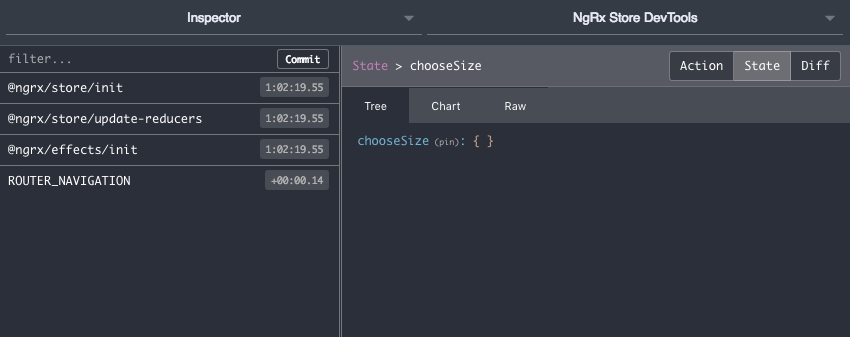
\includegraphics[width=13cm, height=9cm]{ngrx-store/redux-store}

\maketitle{}
\section{ Ngrx Effects }

\subsection{Ngrx Effects - A Primer}
Ngrx effects can be one of the more ambigious parts of the ngrx stack. They are
by definitition something that is supposed to happen when something else has
happened. It will listen for a particular action, and true to Ngrx, return an
observable. In this observable one will have the option to do whatever they want
as well as publish(return) to the action stream.

The line, however, can be blurred, however, as to what the difference is between
an ngrx/effect and a ngrx/store. It is therefore important to distinguish for
architectural reasons. In addition, it can be difficult to determine the
different use cases wherein someone would use an effect. It can indeed be a
slippery slope wherein when to use an effect.

\subsubsection{ Code Example }
\begin{lstlisting}
@Effect({ dispatch: false })
 userDeleted$ = this.dataPersistence.fetch(
   UserActivitiesTypes.UserDeleted,
   {
     run: (action: UserDeleted, state: UserStateModelState) => {
       this.snackBar.open('User Deleted', 'Ok', {
         duration: 2000,
         verticalPosition: 'top',
       });

       return null;
     },

     onError: (action: ActivityDeleted, error) => {
       console.error('Error', error);
     },
   }
 );
\end{lstlisting}

This code example, is a great example as to when someone might use an effect.
As we can see here, we have an action that is being triggered for when a user is
deleted. We then have an effect who's sole purpose to have a snack bar open
when action is called.

\subsubsection{ The Three Pillars of an Effect }
As we discussed earlier, knowing when to use an effect can be a tricky thing to
decipher. Think of it as having the ability to do the following:
\begin{enumerate}
  \item Hook into State.
  \item Ability to do whatever when action is called.
  \item Publish an action back into the state management cycle.
\end{enumerate}

In our scenario, for deleting a user we had two effects:

We called a GraphQL service to delete a user. We then retrieve the result
returned by the GraphQL service, and trigger another effect, which is our
snackbar effect. Yes, this logic can potentially be handled by our view layer
within our component. In addition, we can use the service directly. However,
having all of this logic encapsulated in our effect makes everything very
clean.

\subsubsection{ Further Reading }
While this is out of the scope for this book, I would like to suggest further
reading. Naturally, they would be articles that I would discuss on:
\begin{itemize}
  \item Use cases for using Effects.
  \item Use cases for NOT using Effects.
\end{itemize}

The article for use cases with regards to using effects is \href{"Understanding NgRx
Effects and the Action Stream"}{https://medium.com/@tanya/understanding-ngrx-effects-and-the-action-stream-1a74996a0c1c}.
The articl with regards to use cases in which NOT to use effects is
\href{Stop using ngrx/effects for that}{https://medium.com/@m3po22/stop-using-ngrx-effects-for-that-a6ccfe186399}
These two articles along with the information from this chapter. You should be
well along your way for architecting solid ngrx/effects.

\maketitle{}
\section{ State Management - Properly Unsubscribing }

In Angular, when using ngrx when trying to pull in data, using the async pipe is
the preffered approach. It will handle both the subscribe and the unsubscribe
from the observable pipe for you.

\begin{lstlisting}
<div>{{ observableStream$ | async }}</div>
\end{lstlisting}

\subsection{ What to do When Async Pipe is Not an Option }
There are times When the process of subscribing and unsubscribing must be
managed manually. In this case the recommended approach is to create an
observable that emits when the component is destroyed, and use the rxjs
takeUntil operator to handle the act of unsubscribing for you.

\maketitle{}
\section{ Re-Usable State - An Anti-Pattern }

Creating re-usable state in an Angular application might be one of the most
singular important architectural decisions you might also make. In addition, it
will probably be the longest lasting architectural decision you might make, as
redux is something which is pretty agnostic across many different frameworks.

\subsection{Why Create Re-usable State?}
If there is a singular component that is going to be used across a different
page, having re-usable state, will greatly simplify the architecture. The
logic for reducers can be created once. That logic can then be re-used numerous
times within your app. However, I would like to express how having re-usable
state in @ngrx/store is an anti-pattern.

\subsection{Re-usable State - An Anti-Pattern}
Let's imagine that you have a re-usable data-table, that you would like to use
on numerous pages. There are certain pieces of logic that you want to use with
your state. For instance, you want to create a reducer to determine which
rows have been selected, and if all have been selected. If all has been
selected, then it is moved over to the selected key/value. This logic you have
decided should be mover over to state, so that it can re-used within the data
table, so that it can be passed around and re-used within the app time and time
again.

The only issue with re-usable state, is that as soon as you are using re-usable
state, you are recognizing that the component has to be re-usable. As soon as
you are saying the component is going to be re-usable, you are recongnizing
that there is need for there to be a dumb component and a smart component. As
soon as you are saying there is going to be a dumb component, then any logic
relating to the interface should remain within the components logic it's self.
Therefore, the only state that you will be needing, is the data that is loaded.
That part of state is simplified to a great extent, to where it makes sense to
have state unique per each page.

\maketitle{}
\section{ Facade Pattern }

\subsection{ What is the Facade Pattern? }
The facade pattern is a classic. Anyone who has read the GoF book \footnote{
which if you haven't you should probably take a look.} knows that it is a
mainstay of computer science. Quoting from the GoF book:

\say{A facade is an object that provides a simplified interface to a larger body
 of code, such as a class library.}

\subsection{ A Look at your Typical Non Facade State Pattern  }
This pattern is particularly advantageous when it comes to ngrx actions. If I
may, let's imagine we have the following action:

\begin{lstlisting}
  // choose-size.actions.ts
export class LoadChooseSize implements Action {
  readonly type = ChooseSizeActionTypes.LoadChooseSize;
  constructor(public payload: any) {}
}
\end{lstlisting}

Now any time that we have to call an action we have to do two things:
\begin{enumerate}
  \item Have a store select within the component.
  \item Call a dispatch.
\end{enumerate}

\begin{lstlisting}
  chooseSize: Observable<any>;
  // choose-size.component.ts
  import { Store } from '@ngrx/store';
  constructor(private store: Store<any>) {
      this.chooseSize = store.select('chooseSize');
  //..
  merge(
    this.updateSize$.pipe(
      map((value: any) => new ChooseSizeUpdated(value))
    )
  ).subscribe(action => {
    store.dispatch(action);
  });
\end{lstlisting}

Obviously, this is quite a bit of overhead. Using the facade pattern let's see
if we can simplify this process.


\section{ Constants }

\subsection{ What is a Constant? }
In Javascript the idea of having a constant would be assigning a variable, to a
particular value. Whenever we would like that value, instead of typing out the
value, we would use the variable. At first, however, it might seem
counter-intuitive. Why use the constant value, if it is literally named the same
thing as the actual value?

\begin{lstlisting}[caption=Example of a Constant]
// Update last updated value to have latest payload data
const LAST_UPDATED = "LAST_UPDATED";
new updateValue(payload, LAST_UPDATED);
\end{lstlisting}

\subsection{ Benefits of a Constant }

\subsubsection { Creates a Table of Contents }
When one creates a series of constants in particular file for a certain
component, one can peruse through the constant file, being able to see all
actionable items in one. For instance, the following:

\begin{lstlisting}[caption=Example of a Constant]
// imagine these constants, are in a folder called ValueActionTypes
const UPDATE_VALUE = "UPDATE_VALUE";
const ADD_VALUE = "ADD_VALUE";
const DELETE_VALUE = "DELETE_VALUE";

//imagine the following code is in a new folder called valueActions
import * as types from "../ValueActionTypes";
import {BuyerValue} from './buyer-filter.interfaces';

export class UpdateValue implements Action {
  readonly type = UPDATE_VALUE;

  constructor(public payload?: BuyerValue, public keyName?) {};
}

export class AddValue implements Action {
  readonly type = ADD_VALUE;

  constructor(public payload?: BuyerValue, public keyName?) {};
}

export class DeleteValue implements Action {
  readonly type = DELETE_VALUE;

  constructor(public payload?: BuyerValue, public keyName?) {};
}
\end{lstlisting}

\subsubsection { Communicate to Maintainers }
If using a constant value, it signifies to future maintainers of your code, that
this is a value which is immutable. Further distinguishing intent of
application/snippet of code.

\subsubsection { Helps Secure Values }
When typing in a string for a particular constant value, particular diligence
must be applied in order to make sure it is type appropriately. Typing in the
one place, allows the developer to type in one place, and simply copy and paste
value, from a singular expected location(the const file) to 5 different places.

\maketitle{}
\section{ Enums as Constants }

When working with Typescript, which if you are using Angular, then you most
definitely are using Typescript \footnote{I look forward to working with
Reason sometime soon for typechecking, but I digress.}. Care must be taken to
look into all the nuances that Typescript can offer.

\subsection{ In a non Typescript Setting }

In order to define a constant in a non-Typescript setting, we use the const
declaration to define variables:

\begin{lstlisting}
  const UP = "UP";
  const DOWN = "DOWN";
  const LEFT = "LEFT";
  const RIGHT = "RIGHT";
\end{lstlisting}

\subsection{ Enums an Introduction }
Simply put, Enums allow us to define a set of named constants
\footnote{https://www.typescriptlang.org/docs/handbook/enums.html}.

\begin{lstlisting}
  enum PlaneActionTypes {
      Up = "[Plane] Up",
      Down = "[Plane] DOWN",
      Left = "[Plane] LEFT",
      Right = "[Plane] RIGHT",
  }
\end{lstlisting}

\subsection{ Benefit of Enums over Constants }
Enums allow us to organize a collection of related values. Think of them as
a class for values, wherein the value can only be a string , or number.

\subsection{ Current quirk of String Enums }
String Enums, as opposed to number Enums, have to be constant initialized
with a string literal. To clarify, you might want expect the following to work:

\begin{lstlisting}
  const prefix = '[Button]'
  enum Direction {
      Up = `${prefix} UP`,
      Down = `${prefix} DOWN`,
      Left = `${prefix} LEFT`,
      Right = `${prefix} RIGHT`,
  }
\end{lstlisting}

However, this does not work , because this is not a string literal, i.e. string
only.

\subsection{ Convention as a Result of Quirk }
As a result of quirk, we need a way of specifying that this action is happening
in relation to a specific object. Even though we do have a set using enums,
when identifying the string on it's own, from a state management (dev tool)
perspective, or console perspective, it will be beneficial to have the string
literal, be explicit on it's own. [Screenshot of a redux devtool would great].
Please reference above subsection, "Enums as an Introduction", for how this
translates to code in principle.

\subsection{ Side Note - Why No All Caps in Enums? }
A const in Javascript can actually be re-assigned to something else. For
instance:
\begin{lstlisting}
const PLANE = 'blackbird';
PLANE = 'thunderbird';
// barf
\end{lstlisting}
It is therefore a good convention when using a const, to put it in all caps,
when the value is not attend to be re-assigned such as:
\begin{lstlisting}
const PLANE = 'blackbird';
// woh, I was about to re-assign plane to thunderbird for some weird reason, but
// then I saw PLANE in all caps, so I didn't do it
\end{lstlisting}

However, this is not the convention with Enums, of course, because all enums
are never re-assigned. It is therefore not necesary to to write in all caps.


\section{ Integrating ngrx/store with Apollo Client }
In many architectures, it is most likely going to make sense that it is
microservice based. That is, your data will be served over a slew of different
apis. In which case the intent is that in a regular application, you will be
using GraphQL. It is reccomended that you use Apollo Client as well. We will
cover real quick, how to integrate GraphQL with Apollo Client.

\subsection{ What is GraphQL }
GraphQL is a backend data query language. It will allow you to use a query to
make a request, as opposed to having to supply, url, endpoint, and type of
request.

\subsection{ The Benefit of Apollo }
Apollo is a GraphQL client, used to help ease use of GraphQL http requests
within app. In particular:
\begin{enumerate}
  \item Allows the application developer to easily execute GraphQL queries, and
  configure transport-specific features like headers.
  \item Ensure that all GraphQL results currently being displayed in an app, are
   consistent with one another.
  \item Provide flexible ways to update the cache with results from the server
  when using mutations, pagination, subscriptions, and more.
\end{enumerate}

\subsection{ Dilemma When Using Apollo Client with @ngrx/store }
Apollo will create it’s own inMemoryCache, without dependency on Redux. However,
this creates two separate stores within the app when using @ngrx/store.
One for ngrx/store, and another for the Apollo client. It would be much easier,
obviously, if we had a singular cache/store, for the app.

\subsection{ Enter apollo-angular-cache-ngrx }
apollo-angular is a series of packages for the integration of the Apollo client
with Angular. apollo-angular-cache-ngrx is a package officially a part of one of
the apollo-angular packages. It solves this exact problem, and allows one to use
@ngrx/store as one’s Apollo Cache. (The following can be seen in the github
README.md for the apollo-angular-cache-ngrx repo, but going to put here for
convenience reasons).

\subsection{ Installation }
We will be wanting to install the entire apollo suite at this time.
\begin{lstlisting}
npm install apollo-angular apollo-angular-link-http apollo-link apollo-client graphql-tag graphql --save
\end{lstlisting}
As well as apollo-angular-cache-ngrx
\begin{lstlisting}
npm install apollo-angular-cache-ngrx —-save
\end{lstlisting}

\subsection{ Usage }
\begin{lstlisting}
import {StoreModule} from '@ngrx/store';
import {
  NgrxCacheModule,
  NgrxCache,
  apolloReducer,
} from 'apollo-angular-cache-ngrx';

@NgModule({
  imports: [
    StoreModule.forRoot({
      apollo: apolloReducer,
    }),
    NgrxCacheModule,
  ],
})
class AppModule {
  constructor(ngrxCache: NgrxCache) {
    const cache = ngrxCache.create({});
  }
}
\end{lstlisting}

If one were to now make an Apollo GraphQL query in your Typescript component,
your current ngrx/store will be populated with the appropriate Apollo data.
You will be able to subscribe to it as usual. For instance:
\begin{lstlisting}
  constructor(store: Store<any>, private apollo: Apollo) {
    this.store = store;
      apollo
        .query({
          query: gql`
            {
              users {
                status
                id
                name
              }
            }
          `
        })
        .subscribe((initialData: any) => {
          console.log(this.initialData);
        });
  }
\end{lstlisting}

At this time however, we are not using GraphQL within the above fashion.
Nonetheless, your average app, will be using this sort of architecture, and it
is very good to be aware of it, as well as how to use it.

\subsection{ Bonus - Using Fetch Policy with Apollo }
In apollo, there is the option to specify the fetch policy with regards to
cache. For instance, in your

\begin{lstlisting}
  const fetchPolicy = 'network-only';
  const userActivities$ = this.apollo
    .query<any>({ query, variables, fetchPolicy })
\end{lstlisting}

Doing the above, will not cache your query. Therefore, if you have data, which
will need to re-loaded once a request is made after initial load, using a
fetchPolicy with network only, is the reccomended approach.

\maketitle{}
\section{ Sockets }

When using caching withing an angular application, the first and only dillema
that will come to play is how update that cache. For most applications,
especially the nature of Angular, is that it will the data will need to be
updated frequently.

\subsection{ Understanding Internals of Sockets }
Sockets are that way of updating a cache. It sets up a hook
to the server, so that whenever the server is ready to respond it does. You
might be familiar with this, if you've had a network request that's taken a
while to return it's request. Sockets are like that. When ever the cache has
been updated, another socket goes out, to get it's data when needed.

\maketitle{}
\section{ Apollo Caching with Sockets }

I would like to re-iterate, because I like you the reader, that the value of
being aware of architecture is twofold. One is that one has the option of
preventing future catastrophies. In addition, one has the ability to quickly
put together the correct solution, and have in available in a time intensive
setting. Caching with Apollo is exactly that scenario. One might include
caching, but realize that sockets is something that we would like included with
the app. As a result, the development team might decide to throw away caching,
so that data can be updated. I would like to say that it is very much possible.
I would also like to lay out, what in a couple of paragraphs that best strategy
to do so within Apollo.

\subsection{ Apollo Caching with Sockets }
\mybox{One side note, is that it will generally be a requirement that will
come from front end first, that they will need to use something like sockets.
However, backend will also need to setup websockets, in order to get everything
to work as expected.}

It should be noted that GraphQL offers three types of data queries:
\begin{itemize}
  \item Query
  \item Mutation
  \item Subscriptions
\end{itemize}

Subscriptions in particular is very similar to websockets. 

The package at this point which makes the most sense is
\href{subscriptions-transport-ws}{https://github.com/apollographql/subscriptions-transport-ws}

// TODO Add more content here

\maketitle{}
\section{ Apollo Client Middleware }

Middleware in general is a concept in many different plugins. In general, it
means a service layer one can put on top of application in question. In
particular, for an Apollo application, it will allow us to intercept the
current request, and put in whatever we want.

\subsection{ Middleware as Architecture }
Middleware can be considered architecture, because some plugins may not support
middleware. In addition, even if they do support middleware, it might not be so
apparent from documentation how one might go ahead and do so. So much so to the
extent, that it will considerably slow down development, and a conversation will
have to be had if research is worth it.

\subsection{ Middleware in Apollo }
Apollo has a number of quirks with regards to it's middleware. For now, it adds
typename to every query request. This can cause issues when it comes to unit
testing. Let's create middleware to remove typename from the app:
\begin{lstlisting}
const stripTypenameMiddleware = new ApolloLink((operation, forward) => {
  if (operation.variables) {
    operation.variables = omitDeep(operation.variables, '__typename');
  }

  return forward(operation);
});
\end{lstlisting}

Here we are stripping typename from the application.

\subsection{ Adding projectId to Requests }

Using middleware, we have the option to add a projectId to our requests. Let's
say that we need the data coming back to be specific to a certain project.
Instead of having to inject that on a request per request basis, we would like
to go ahead and have apollo inject projectId as one of the query requests.
\begin{lstlisting}
const attachProjectIdentifiers = new ApolloLink((operation, forward) => {
  combineLatest(
    this.projectFacade.projectId$
  )
    .pipe(first())
    .subscribe(([projectId]) => {
      operation.variables = {
        ...operation.variables,
        projectId: projectId,
      };
    });

  return forward(operation);
});
\end{lstlisting}

In this fashion, one can eliminate clutter from apollo requests. In addition,
one can alter apollo to have specific items in the response if need be. 


\section{ Interfaces and Unions }

In GraphQL, and more in particular, because we are working on things from the
UI side of things, a Union type gives us the ability for one field to contain
more than one field. The best way to really think of it, is in terms of
Typescript. A union type would be:
\begin{lstlisting}
  type Book {
    title: String
  }

  type Author {
    name: String
  }

  type Result = Book | Author;

  type Query {
    search: [Result]
  }
\end{lstlisting}

As we can see, it is telling us that it can be one, of the other with regards
to data type. So instead of returning irrelevant data, we only return the data
we need. This is beneficial for a number of reasons.
\begin{enumerate}
  \item It lightens payloads
  \item Allows for succint sorting, on front end. I.e. do not have to sort from
  the backend.
\end{enumerate}

\subsection{ Using Unions with Apollo Client }
This is where at this time, things start to get really interesting. Using Apollo
with unions/interfaces starts to become tricky. In particular, the client has
no idea what is going on from the server side of things. Once we have different
sorts of data for a singular query coming back based on the type of data
avaialable, Apollo Client will just assume it is a certain type if it returns
all data for a specific type.

Apollo made the decision to use something called the
IntrospectionFragmentMatcher. It will look something like this:
\begin{lstlisting}
const fragmentMatcher = new IntrospectionFragmentMatcher({
  introspectionQueryResultData: {
    __schema: {
      types: [
        {
          kind: 'INTERFACE',
          name: 'User',
          possibleTypes: [
            { name: 'User' },
            { name: 'UserWithReason' },
            { name: 'UserWithRound' },
            { name: 'UserWithBid' },
          ],
        },
      ],
    },
  },
});
\end{lstlisting}

It tells Apollo Client for Angular that it expects the above types in the
interface for User. Where it starts to get really interesting is that Apollo
Client requires for IntrospectionFragmentMatcher to be used regardless. So, in
their documentation they reccomend that a script be used at build time, that
creates a JSON file. This JSON file should then be used in the
IntrospectionFragmentMatcher. This is very cumbersome, because if backend
decides to throw something in for an already existing interface, it will cause
the backend to break for that query.

I would like to repeat this once again, if you do not have an
IntrospectionFragmentMatcher set up in your app, and backend adds union, or
interface types, it will cause that data to break, and it will return an empty
object.

\mybox{
  It should be noted, that one might immediately think, why not go ahead and
pull in the data for possibleTypes at runtime, and then use that for the
IntrospectionFragmentMatcher? The difficult part about it, is that the way
apollo works for the IntrospectionFragmentMatcher, is that it requires it to be
passed into the cache. The cache is created on page load, and then having to
update after cache is loaded, well you already missed the boat. So within the
context of Apollo Client for Angular, the only way to load in possible types
is to go along with the way documentation reccomends it.
}

\subsection{ What to Know Ahead of Time }
What would be really helpful to know ahead of time, is that this is an issue
that can only be solved by DevOps. It requires that back end and front end are
built at the same time. That way, they both get pushed only once the new script
is there. In this sitution, there really is no way about it. Having a mono repo
architecture across your company will greatly alleviate this process.
\footnote{I have created this issue to bring awareness to this \href{https://github.com/apollographql/apollo-client/issues/4202}{issue}, but nothing so far}

\maketitle{}
\section{ Integrating a Component with @ngrx/store }

Another chapter has been dedicated solely to integrating a component
with @ngrx/store. This is because it is a cookie cutter process. Observables
are notoriously known, for abstracting events, and therefore allowing the same
code to be repeated time, and time again. The following is what can be expected
to be repeated time and time again in your application, after initially
generating files.

Just for redundancy sake, there are six steps, that go into setting up state
with any given component, that are handled by the nx ngrx cli:
\begin{enumerate}
  \item Store
  \item Action
  \item Store
  \item Reducer
  \item Initial State/Enums\footnote{In some other framework it might be constants}
  \item Effects
\end{enumerate}

All that is left, is for us to now to do three things component side:

\begin{enumerate}
  \item Set ups actions in view layer (i.e. HTML)
  \item Select store, so that it can be used in component
  \item Setup subject in component, so that it can be used with actions in view layer
  \item Set up subscribe in component(to transfer model to controller) \footnote{A subscriber is rarely setup in the smae component setting up the store to begin with}
\end{enumerate}

This is pretty standard, and this will be done in every standard application.
It is this simple, and will follow this formula, and yes, you should be in shock
in how seamless integrating state management technology is at this point,
because I am.

\subsubsection{ Re-iterating purpose of book }

I would just like to re-iterate, that the point of this book, is to go through
the architecture of the entire angular ecosystem. So that someone can read this
book and have the confidence that they are building their Angular app the proper
way, and that they do not have to look elsewhere. That being said, I will not be
going into the whole code base of what is happening. However, I would like to show
an example of along the lines of what will end up happening.

\subsubsection{ Creating a subject }

To re-iterate, what is a subject? It is both an observable and an observer?
\begin{enumerate}
  \item Observer — It has the next, error, and complete methods.
  \item Observable — It has all the Observable operators, and you can subscribe
  to him.
\end{enumerate}

Therefore, in an Angular setting, using @ngrx/store, subjects are our friends. It
allows us to have a singular event handler, to be used by all html event handlers
within component. In addition, it gives us a subscribe. The general pattern in
an Angular app will be as follows:
\begin{enumerate}
  \item Create subject in component
  \item Set up different namespace for unique actions in components
  \item Merge subjects into singular subscribe
  \item Which then emits payload per action
\end{enumerate}

\subsubsection{ Creating a Subject - Code Dive }

\maketitle{}
\section{ Unit Testing }

Unit testing has always been a hot topic. It's because it really isn't so well
understood amongst many software engineers. In addition, I know of many managers
who look as unit testing as icing on the cake. Good unit testing, is incredibly
difficult, and requires incredible amounts of due dilligence. Many books have
been written in this regard, and will not go into detail here.

However, what unit testing allows us to do, is assure the code we are
implementing is correct. Just as important, it sets testing in place, so that if
another developer changes something, such as the ordering of function
parameters, a class name, or a result of a function it will break. Unit testing
can also be set in place to make sure a certain function is called, when a
button is clicked, or in what order functions are correct. In can be set in
place as automatic self correcting code.

Unit testing, can also make our code self documenting. In addition, it can
give us the confidence moving forward knowing that this will work the way it
needs.

Unit testing really is a beast, and is really hard to manage. It's because it
isn't directly related to quality assurance, and can easily go under the radar,
as the app will go on without it. However, everytime that I have communicated
with management the bottom line. Research has been done on unit testing, and that
the application will be harder to manage long term, without it, they understand.
Bring the above point up to them, and hopefully you can have unit testing as a
part of your application.

At this point in our application, the only thing that we have created that
deserves to be unit tested, are the reducers. Let's go ahead and unit test those:

\begin{lstlisting}
describe('Functionality for the ChooseSizeUpdated reducer', () => {
  const chooseSizeData = {
    columns: 20,
    rows: 20,
    pixelSize: 20
  }
  it('should update the chooseSize store as is approprate', () => {
    const action: ChooseSizeUpdated = new ChooseSizeUpdated(chooseSizeData);
    const actual = chooseSizeReducer(initialState, action);
    expect(actual).toEqual(chooseSizeData);
  });
});
\end{lstlisting}

The above is an example of what a sample unit test for a reducer would look like
in the chooseSizeUpdated reducer.

Note: Add in section going over best conventions with regards to unit testing.

\maketitle{}
\subsection{ Unit Testing as a Discipline }

Unit testing is difficult, because it is a different discipline. In particular,
the above unit testing that we made, is a great example of poor unit testing.
We simply tested to make sure that all fields properly made their way over.

However, there are a number of considerations to keep in mind:
\begin{enumerate}
  \item What happens if we insert a string, instead of a number?
  \item Is there any limit on the number of rows, or columns?
  \item Should there be a limit on pixel size?
  \item Should there be a 1:1 ratio between rows and columns, or vice versa?
\end{enumerate}

\subsection{ The Irony of a Product Engineer }
One might think that the above requirments, are to be pro-offered by the Product
and to be tested by QA. However, at the end of the day, if these issues exist,
it will mean that the software you created will be lackluster. [This indeed
extends to other parts of the app, however, we are currently focusing on
unit testing]. Therefore, try to take ownership as an engineer. There are
different levels of intelligence, but amongst many other things, software
engineers are a truly analytical bunch.

\maketitle{}
\section{ Jest }

\subsection{ A Primer. }
Jest is a test runner created by Facebook to allow for the "Delightful
Javascript Testing".

\subsection{ The Benefits of Jest Vs. Karma }
\begin{enumerate}
  \item Fast and sandboxed
  \item Built-in code coverage reports
\end{enumerate}

\subsubsection{ Fast and sandboxed }
Jest parallelizes test runs across workers to maximize performance.
Console messages are buffered and printed together with test results. Sandboxed
test files and automatic global state resets for every test so no two tests
conflict with each other.

\subsubsection{ Built-in code coverage reports }
One has the ability to create code coverage reports using --coverage.  No
additional setup, or libraries are needed. Jest can collect code coverage
information from entire projects, including untested files. The way it moves
focus away from something like istanbul is fantastic. The UI, in my humble
opinion, for what it's worth, is not the greatest.

\subsubsection{ Does not require starting a Browser }
This one in particular helps with regards to CI/CD. Not requiring a browser,
does not require a browser to be built into the CI/CD. In addition, a large
part of performance issues with regards to unit tests, is having to start the
browser every time.

\subsection{ Using Jest within an Nx Setting }
\begin{verbatim}
  ng generate jest
\end{verbatim}

\begin{verbatim}
  ng generate jest
\end{verbatim}

After running the above generator, one can now run jest within your app. When
generating a lib, one can now do:
\begin{verbatim}
  ng generate lib libname --unit-test-runner jest
\end{verbatim}

\footnote{If you are coming from an existing nrwl workspace, please use the
following blog post to find out how to upgrade to Jest https://blog.nrwl.io/nrwl-nx-6-3-faster-testing-with-jest-20a8ddb5064}

\subsection{ Primer on Jest Syntax }
Real quick, I would like to go through a couple of things that Jest offers over
Karma.

\maketitle{}
\section{ Unit Testing Architecture }

In any given UI application, the following should be considered as appropriate
architecture.

\begin{enumerate}
  \item Testing structure
  \item Assertion functions
  \item Generate, display and watch test results
  \item Generate and compare snapshots of component and data structures to make
  sure changes from previous runs are intended
  \item Provide mocks, spies, and stubs
  \item Generate code coverage reports
  \item Provide a browser or browser-like environment with a control on their
   scenarios execution 
\end{enumerate}


\section{ Interfaces and Unit Testing }
In unit testing it can be very difficult to keep in sync the mocked data you
are using, with actual data used within app's actual live UI. The easiest, and
most efficient way of doing this is creating interfaces. The part where it
becomes tricky, is that generally data is used in multiple places. For instance,
we might have state that is contained in a separate component, wherein the data
originates from can be somewhere else. In addition, the data might also be used
in some other component as well as in some other service.

\subsection{ In Sync Data - Interface Architecture }
An interface at it's core is responsible for making sure that data follows a
pre-described schema. The part, however, that is unintuitive in an Angular
setting, is what happens when you have services, components, state, and spec
files all vying for the same data. Do we use one interface for all of them,
or different one's for each file group? If we do end up using one interface,
what sort of data structure is it that we will use for all of these files.

\subsubsection{ Interface Architecture - The Dillema }
As we discussed in the previous paragraph, in an Angular application, there will
be services, components, state and spec files vying for the same data. The
dillema when it comes to interfaces, however, is that they need data in
different ways. I would like to layout this data in detail.

Let's imagine that we have a data-table that we need to specify data:
\begin{itemize}
  \item Service - Used to determine status of checkbox logic. It only needs to
  know length of data, and actual data is irrelevant. Respective spec, only
  needs to be aware of similar data.
  \item Component - Needs to know actual data, so that it can pass along
  observable stream component html. Respective spec needs to be aware of data.
  \item State - Depnding on the reducer, or effect, it might need all of the
  data, or none of it. Respective spec will need to familiar of similar data.
\end{itemize}

\subsection{ In Sync Data - The Solution }
As one can see, it is actually counter-intuitive to create a singular interface
for one's service, state, component(s), and their respective specs. However, if
one does not use the same singular spec for all of them, one runs the risk of
them getting out of sync with each other. The data inside of the object might
make all the difference when it coems to causing unit tests to fail.

The solution is as follows. There should be a singular interface that exists
for the root of the following files:
\begin{enumerate}
  \item Services[Includes spec files]
  \item State[includes spec files]
  \item GraphQL(Interfaces not used, but influenced by, and therefore important
  to be in the same directory)
  \item Component(Not in same folder as above)
\end{enumerate}

This, however, requires that all the files be tightly coupled together. In order
to do this, we must create a well thought out folder/file structure. This is
what we will be calling Data Access architecture.

\subsection{ Data Access - Folder Structure }
Let's say we are creating an grid-form component, that will make use of backend
data. The data structure will look as follows:

\begin{forest}
[app-name-goes-here
  [data-graphql
    [src
      [lib
        [fragments
          [\/*.fragments.ts,file]
        ]
        [queries
          [\/*.queries.ts,file]
        ]
        [mutations
          [\/*.mutations.ts,file]
        ]
      ]
      [\/index.ts,file]
    ]
  ]
  [data-models
    [src
      [lib
        [\/*.interfaces.ts,file]
        [\/*.mocks.ts,file]
      ]
      [\/index.ts,file]
    ]
  ]
  [data-services
    [src
      [lib
        [\/*.service.ts,file]
        [\/*.service.spec.ts,file]
      ]
      [\/index.ts,file]
    ]
  ]
]
\end{forest}

The expectation is that there will also be a sister folder/file structure
for these three in particular(data-graphql, data-models, data-services). In the
appropriate feature, it will have a state feature, which will have the same
name as the respective data-access architecture.

\begin{forest}
[user
  [src
    [lib
      [user
        [\/user.component.html,file]
        [\/user.component.scss,file]
        [\/user.component.spec.ts,file]
        [\/user.component.ts,file]
      ]
      [+state
        [\/user.action.ts,file]
        [\/user.adapter.ts,file]
        [\/user.effects.spec.ts,file]
        [\/user.effects.ts,file]
        [\/user.facade.spec.ts,file]
        [\/user.facade.ts,file]
        [\/user.reducer.ts,file]
        [\/user.selectors.ts,file]
      ]
      [\/px-user.module.spec.ts,file]
      [\/px-user.module.ts,file]
    ]
    [\/karma.conf.js,file]
    [\/tsconfig.lib.json,file]
    [\/tsconfig.spec.json,file]
    [\/tslint.json,file]
  ]
  [\/index.ts,file]
  [\/test.ts,file]
]
\end{forest}

Using this folder/file structure, we can enforce there being a single interface
used across all files within our app that are using data. The idea is that the
nomenclature will remain the same across

\subsection{ Example of How Interface Might Be Used in Real Time }
Now that we have our folder/file structure in place, we can prove how having a
singular interface can be used to make sure all of our files are in sync.

\begin{lstlisting}
export interface GridForm {
  column: string;
  row: string;
  pixelSize: string;
}
\end{lstlisting}

\subsection{ Example of How Data Mock Will Look Like }
In addition to our interface, we will have mocked data that will be used in a
number of different instances. It makes sense to have data in a mock.ts file
so that it can be re-used throughout app, without having to re-create.

\begin{lstlisting}
cost GridForm = {
  column: '20';
  row: '20';
  pixelSize: '20';
}
\end{lstlisting}

\subsubsection{ Service for Pulling in Pre-Populated Grid Form }
In our service, we will use the interface to determine what sort of data we
expect to be pulled in.

\begin{lstlisting}
getGridForm(projectId: string): Observable<GridForm> {
  const query = GridFormQuery;
  const variables = {
    projectId
  };

  const form$ = this.apollo.query<GridForm>({ query, variables });

  return from(buyers$).pipe(pluck('data'));
}
\end{lstlisting}

\subsubsection{ Service Spec for Pulling in Pre-Populated Grid Form }
In the spec for our service, we will have one consistent piece of data that will
be used throughout the service spec:
\begin{lstlisting}
const gridForm: GridForm = {
  column: "20";
  row: "20";
  pixelSize: "20";
};
\end{lstlisting}

Here we are using the interface to make sure that the mocked data used with the
service stays true to the data that is expected to be returned. If the data
ever changes in actual app, the interface will be there to make sure our specs
data mocks are up to data as well.

\subsubsection{ Reducer for populating state with appropriate Grid }
For simplicity sake within our app, we are going to take the data as is, and
pass it directly into our store to be used within app:
\begin{lstlisting}
export function gridFormReducer(
  state: GridForm,
  action: BuyerAction
): GridForm {
  switch (action.type) {
    case BuyerTypes.FormLoaded: {
      return {
        ...state
      };
    }
  }
}
\end{lstlisting}

Here we have the interface telling our app that all data within our reducer
must consist of the three items we have specified in our GridForm interface.

\subsubsection{ Reducer Spec for populating state with appropriate Grid }
\begin{lstlisting}
  describe('gridFormLoaded action', () => {
    it('should populate the buyer entities and ids', () => {
      const action = new FormLoaded(gridForm);
      const state = gridFormReducer(initialState, action);

      expect(state).toEqual(gridForm);
    });
  });
\end{lstlisting}

Here we have a very simply unit test that once again has the same data that is
used across the app. By having an interface and using it for the data within the
interface we can make sure that the data for the reducer spec is up to date with
actual app.

\subsubsection{ Effect for populating state with appropriate Grid }
\begin{lstlisting}
@Effect()
loadGridForm$ = this.dataPersistence.fetch(BuyerTypes.LoadGridForm, {
  run: (action: LoadGridForm, state: GridForm) => {
    const projectId = this.projectFacade.getProjectIdFromState(state);

    return this.service
      .getGridForm(action.payload, projectId)
      .pipe(map((gridForm: GridForm) => new GridFormLoaded(gridForm)));
  },

  onError: (action: LoadGridForm, error) => {
    console.error('Error', error);
  },
});
\end{lstlisting}

In our effect, using the facade pattern \footnote{it is calling the effect,
pulling in data, and then having the appropriate action fired off, for saying
data is loaded}. In our param for state, the most data heavy part of our effect,
we are once again using the same interface.

\subsubsection{ Effect Spec for populating state with appropriate Grid }
\begin{lstlisting}
const projectId = '123';

describe('loadBuyers$', () => {
  beforeEach(() => {
    spyOn(service, 'getGridForm').and.returnValue(of(gridForm));
  });

  it('should work', () => {};
    const action = new LoadBuyers();
    const completion = new BuyersLoaded(gridForm);

    actions$ = hot('-a', { a: action });
    const expected$ = cold('-c', { c: completion });

    expect(effects.loadGridForm$).toBeObservable(expected$);
    expect(service.getGridForm).toHaveBeenCalledWith(projectId);
  });
});
\end{lstlisting}

Here we are once again attaching an interface for gridForm, our data, so that it
is consistent across our application.

\maketitle{}
\section{ Mocking Data }
An interesting phenomenon that happens within many enterprises, is with regards
to unit tests and maintanability. Many times the data mocks are repititions of
themselves. In addition, utilities with regards to mocking data. I've done this
myself, maybe you have as well. This chapter is simply there to put this in as
convention, to go ahead and edit moving forward.

\subsection{ Function Composition }
With regards to creating re-usable data, there are two options. One can use a
function to generate a mock. Alternatively, one can use a spread operator. For
the most part, I prefer a function to generate a mock. It gives the option to
specify parameters to be passed through.

\begin{lstlisting}
// this interface is in our users.interface.ts file
export interface User {
  id: string;
  name: string;
}
// this interface is in our users.interface.ts file
export interface Users {
  users: User
}

let generateMockData: Users = (data: user) -> {
  users: {
    ...data
  }
}
\end{lstlisting}

By using the simple above function, properly type annotated we have the option
to generate mocked data that is unique to our interface. In addition, we have
the ability to pass in data as it is unique to our specific use case.

\subsection{ Core Constants }
In addition to having function composition tied to our interfaces, odds are that
the data being passed in might have the same signature time and time again.

Enter the three constant rule:

\maketitle{}
\section{ Unit Testing - Event Handling and Text}
In my mind, anything which is considered as architecture is something which
isn't immediately considered as obvious. One aspect of unit testing that tends
to be overlooked, is unit testing event handling. For instance, let's say we
have a filter toggle, wherein we only want the filter to show when a user clicks
on it. This is something which we can trigger from unit tests, without the need
to have go through integration testing. In addition, certain areas of our app
are very sensitive when it comes to text. Focusing on these two alone, allows
our app's integrity to be head and shoulders above the rest.

\subsection{ Angular's best Utility Testing Suite }

TODO

\subsection{ Unit Testing - Event Handling }
Going back to our previous example of a filter toggle, let's jump right in and
see what a filter toggle unit test might look like:

\begin{lstlisting}
const filterToggle = fixture.nativeElement.querySelector(
  '.filter-toggle'
);
filterToggle.click();
expect(component.showFilter).toBeTruthy();
filterToggle.click();
expect(component.showFilter).toBeFalsy();
\end{lstlisting}

We are using querySelector to target the first .filter-toggle html class
(assuming there is only one on the page). Being that our default view is false,
we are using the component.showFilter to make sure that value is truthy when
clicked on. Moving on, when clicked on again, we want to make sure that element
is hidden. \marginpar{consider revision of code, it should target actual element
in addition to code}

We have now completely though the power of unit testing, determined whether, or
not an element is going to show up.

\subsection{ Unit Testing - Determining Text }
With regards to text, let's say that we want to test the entire component at a
specific time period, and want to make sure it contains three different words:
\begin{lstlisting}
it('should show buyer company names', () => {
  expect(fixture.nativeElement.innerText).toContain('Apple');
  expect(fixture.nativeElement.innerText).toContain('Microsoft');
  expect(fixture.nativeElement.innerText).toContain('Google');
});
\end{lstlisting}

Text might seem intuitive. However, there is the option to target text at
different areas of time, and to make sure what one is looking is the correct
format at a given time. Doing something like this takes experience to get it
right. However, assuming you didn't know beforehand, you now know that you have
the option to target text at a specific time.

\maketitle{}
\section{ Unit Testing - Mocking Providers }
Another important part of Angular Architecture, is that one has an option to
import a service as is, or to mock it out. This will apply, as per our
architecture to facades as well. Not doing so, will leave your unit tests at
the mercy of your services, and might have you unit testing your service as
well as your specific component.

\subsection{ Re-iterating Previous Point }
We have already discussed a previous point with regards to unit testing and
interfaces with regards to unit testing. This is indeed a very important point
that works in tandem with mocking providers, and we will touch on this in this
chapter.

\subsection{ Mocking Providers - Setting the Landscape }
Just setting the landscape for what an example situation might be like with
regards to mocking providers. In our Angular - The Full Gamut architecture, we
have a facade which is always going to be responsible for bridging the data
retrieved by our service, with our component:
\begin{lstlisting}
gridForm$: Observable<GridForm[]> = this.store.pipe(select(getGridForm));
\end{lstlisting}

The above ^ is an example snippet of our getGridForm.facade.ts file, that will
be responsible for pulling data from our store, using the getGridForm selector
already specified else where. If we were to pull in this facade as is, it would
end up actually pulling data from the server while doing unit tests! That would
be a cardinal sin.
\begin{verbatim}
<form>
<div>{{ (gridForm | async).row }}</div>
<div>{{ (gridForm | async).column }}</div>
<div>{{ (gridForm | async).size }}</div>
</form
\end{verbatim}

\subsection{ Mocking Providers Within Unit Test - A Primer }
In out unit test in order to mock the above Observable gridForm\$ stream, we
would do the following:
\begin{lstlisting}
generateMockGridForm(): GridForm {
  return {
    row: '20',
    column: '20',
    size: '20',
  }
}

providers: [
  {
    provide: GridFormFacade,
    useValue: {
      gridForm$: of(generateMockGridForm()),
    },
  },
],
\end{lstlisting}

In this very simple scenario, we have just made it so that the data retur

\maketitle{}
\section{ Marble Unit Testing }

Unit testing observables, heck working with obserables is never really easy.
Primarily, it's not the logic one will come across in other parts of one's
application. As opposed to regular logic, where one has the option to simply
console out logic and see what is there, then and there, one does not have that
option wih observables. Observables are a stream and in the context of
javascript it is an object that will a series of functions. In addition, an
Observable as a stream contains more than one snippet of data in it's entire
lifecycle.

\subsection{ Marble Unit Testing - A Primer }
Marble unit testing is a very efficient way of unit testing observables. It
keeps in mind the following:
\begin{enumerate}
  \item Recognizing that an observable stream can emit any number of values
  after a specific set of time.
  \item An observable is always observing until actually complete
  \item It can emit a number of different things at the same time, or at
  completely different times.
\end{enumerate}

\subsection{ Great Example }
Let's imagine that we get back a specific set of data as an observable. However,
within that set of data, we only want ids. Backend is tied, and they do not have
the capacity to give us a pre-poulated set of data for id. Our code will look
something like this:
\begin{lstlisting}
userIds$: Observable<string[]> = this.users$.pipe(
  map(users => {
    return users
      .map(user => {
        return user.id;
      })
  })
);
\end{lstlisting}

\subsubsection{Creating a unit test}
In our unit test, we would like to make sure that when we pass a set of data,
id's are indeed being extracted and returning a new array. We can do something
as follows using marble tests:

\begin{lstlisting}
const usersMock: User[] = [
  {
    id: '123',
    name: 'Charlie',
  },
  {
    id: '246',
    name: 'Lisa',
  },
  {
    id: '369',
    name: 'Harley',
  },
];

it('should return buyer data for tier', () => {
  const expected$ = hot('(c|)', { c: ['123', '246', '369'] });

  expect(component.buyerTiers$).toBeObservable(expected$);
});
\end{lstlisting}

In this unit test, we expect our function to return.
\begin{verbatim}
  ['123', '246', '369']
\end{verbatim}

As we are unit testing against an observable, we can potentially use subscribe,
to emit the value of the component function we are testing. However, this can
get a bit cumbersome, as it's a bit of code, and throwing subscribes into a unit
test can go curious places. In our marble unit test, we can simply say that we
have a hot observable that contains x amount of values.

\maketitle{}
\section{ TDD/BDD }

One of the tricky things with regards to E2E tests, is how it fits into a
TDD/BDD environment. Writing unit tests before we can see anything in our UI
already takes quite a bit of discipline. Adding in an E2E test to the workflow
seems like a bit much? Ok, so let's get into the thick of it. I think we'll all
have a good time!

\subsection{ What is TDD? }

\begin{enumerate}
  \item Start by writing a test
  \item Run the test and any other tests. At this point, your newly added test
   should fail. If it doesn’t fail here, it might not be testing the right
   thing and thus has a bug in it.
  \item Write the minimum amount of code required to make the test pass
  \item Run the tests to check the new test passes
  \item Optionally refactor your code
  \item Repeat from 1
\end{enumerate}

\subsection{ The Benefits of TDD? }
\begin{enumerate}
  \item Higher test coverage. \footnote{Emphasis is put on testing}
  \item Focus
    \begin{enumerate}
      \item Focus one part of issue one of a time.
      \item Allows one to realize when to stop coding.
    \end{enumerate}
  \item Interfaces
    \begin{enumerate}
      \item Allows you to think what is actually being baked into code more
      thoroughly. Allowing for interface to be written from the bottom
      up(behavior, implementation), instead of top down(implementation,
      behavior)
    \end{enumerate}
  \item Living Documentation. \footnote{Not to mention very verbose.}
  \item Enforces Pure Functions - Or re-usable code
    \begin{enumerate}
      \item As pure functions are easier to test, it will cause the developer
      to veer towards writing more pure functions.
      \item If pure functions are not an option, it will nonetheless cause the
      developer to veer towards re-usable code, and re-usable specs. \footnote{
      because this is the developer who is going to have to write tests time
      and time again.
      }
    \end{enumerate}
\end{enumerate}

\subsection{ What is BDD? }
Typically when testing a particular function at a later date, that function can
change it's implementation. For instance, the counter can start at 5, instead of
zero, breaking the expect statement of 1, when it is now 6. In BDD we focus on
the intended behavior, which is adding 1 to a particular value.

First things, first. Which comes first, unit test, or E2E tests? E2E tests will
end up going first, however, we will end up satisfying the unit tests first.

\begin{lstlisting}
// Non BDD
describe('Counter', () => {
  it('tick increases count to 1', () => {
    var counter = new Counter();

    counter.tick();

    expect(counter.count).toEqual(1);
  });
});

// BDD
describe('Counter', () => {
  it('should increase count by 1 after calling tick', () => {
    var counter = new Counter();
    var expectedCount = counter.count + 1;

    counter.tick();

    expect(counter.count).toEqual(expectedCount);
  });
});
\end{lstlisting}

\subsection{ The Benefit of BDD }
If at a later time the counter(as seen above), for instance, has to change
based on requirements(starting at 5, instead of 1), it will not affect the unit
test. That's it plain and simple, almost too simple, hmm... suspicious.

\subsection{ Convincing the Skeptic on TDD/BDD }
One of the equally most difficult things with unit testing, especially in a web
setting is coming across the various use cases, that will slow you down. Trying
to convince management, or whoever is in charge, that the amount of time that
you are spending on your unit tests, is going to validate the time taken towards
writing them. The following are some items that can be used towards convincing
the skeptic.
\begin{enumerate}
  \item Too simple to fail
    \begin{enumerate}
      \item If this is used regularly in our application, doesn't it then make
      sense to spend 5 minutes testing it?
    \end{enumerate}
  \item Too difficult to unit test
    \begin{enumerate}
      \item Good indication that it needs to be re-factored, proving point of
      benefit of unit testing.
    \end{enumerate}
  \item Too time consuming
    \begin{enumerate}
      \item App will produce more bugs.
      \item Lower quality code in regular app.
      \item Lack of confidence, perhaps bugs will be created under the radar.
      \item Lower design of system as a whole.
    \end{enumerate}
\end{enumerate}


\chapter{ Unit Testing TDD - First Princples Discovery }

Unit testing as a discipline is something which is very hard to write. Writing
a good unit test is as much as a discipline as writing good software. In
addition, if someone is following TDD standards, then knowing of all the unit
tests ahead of time can be very difficult. Leading many developers to leave the
TDD environment. If they do write unit tests, it will be towards the end. The
following is a great way, and as far as I am concerned the best way to discover
unit tests.

\section{ What is the First Princples Thinking? }
In Physics\footnote{Not a physicist, but I heard of this concept the first time
from Elon Musk. I am, however, a Talmudist, and in talmud we have a similar
concept called Pilpul}, there is a concept called, first principles thinking.
This means boiling down a priciple to it's essnetial truth and then building up
from there. With regards to Unit Testing, and specifically test driven
development, this principle will help to create fantastic unit tests.

\section{ First Princples Thinking - Rubber Ducking - An example }

\begin{lstlisting}
  Q: What would we like to get out of the choose size form?
  A: We would like to specify number of rows, number of columns, and pixel size.

  Q: Being that these are numbers, do we have any way of preventing
  the user from entering in any value other than an number?
  A: The input will only allow numbers.
  Q: Ok, do you see any value in setting up logic, so that if it is not a
  number, then it will throw an error?
  A: No, because there will never be a situation wherein they can not put in a
  number.
  Q: In that case, should we take a snapshot and make sure input fields are
  indeed of the type number. If not then it should error.

  Q: Now that we have established that these are always numbers, is there any
  limit on the size of this grid.
  A: Not really, I can see it as just being what the window size.
  Q: Hmm, I find that interesting, so you are saying that it can be any size.
  A: Yes for this iteration.
  Q: Okay, but it will be specific to window size.
  A: Yes.
  Q: Ok, so let's go ahead and create unit test, that it should have an
  error, that based on window size, if value is greater, it should automatically
  have it go to the height window size. In addition, there should be test that
  specifies as such.

  Q: Now that we have established that these we constrained window, is there any
  limit on the ratio between column size, and row size?
  A: No.
  Q: Is there any way that we can create a unit test, to just say that it
  passes, if there is a difference in ratio, between, then should not error out?
  A: Yes, need to figure this out though. Not sure how to do off hand.

  Q: Now that we have established that there are no constraints, what else is
  there for us to test. We have covered window size, ratio, input type, what
  about a max pixel Size?
  A: Hmm, why would we care about that?
  Q: Not sure, good point.

  Q: Hmm, that being said, should we only allow pixel size that is within the
  frame of the row and column size? For instance, let's say we have 20 rows, and
  20 columns, should the pixel size be something that perfectly divides into
  400?
  A: Not sure, it would be a lot of overhead at this point.
  Q: Almost feel like we should automatically control pixel size based on column
  and row size.
  A: Ok, out of scope, let's not.

  Q: Anything else?
  A: Not that I can think of.

  //End of Scene - dev takes a bow
\end{lstlisting}

To re-iterate in this book, we will not go into specifics of what is going on
at a particular time. However, these unit tests can be found in the Angular
Pixel Illustrator repo.

\maketitle{}
\section{ Unit Testing Component using Apollo }

Unit testing an app which has a DOM, is always a very difficult process. For
instance, one can be familiar with how a certain technology should be stubbed.
However, how one goes ahead and does so, is unique to that specific technology.
With regards to UI, frameworks currently tend to change very quickly. In
addition, thrre are many different frameworks, many of which use different
testing frameworks. It goes without saying, if I have a chance to learn
something and document it with regards to unit testing, it would be my honor to
do so.

In particular, with regards to the Angular Apollo Client. Until recently
(pre v1.1.0), using Apollo in an Angular App, was a very cumbersome ordeal.
In particular, there was no testing module. One would have to spin it up
themselves. However, now that we are dealing with v1.1.0, there is an official
testing suite set up.

\subsection { Re-visiting Component using Apollo }
First let's look at your standard Angular component generated by the Angular
CLI.

\begin{lstlisting}
import { Component, OnInit } from '@angular/core';

@Component({
  selector: 'ill-color-picker',
  templateUrl: './ill-color-picker.component.html',
  styleUrls: ['./ill-color-picker.component.scss']
})
export class IllColorPickerComponent implements OnInit {

  constructor() { }

  ngOnInit() {
  }

}
\end{lstlisting}

\subsection { Integrate Apollo with Component }

\begin{lstlisting}

+ import { Apollo } from 'apollo-angular';

+  ngOnInit() {
+    this.apollo
+      .query({
+        query: gql`
+          colors
+        `,
+      })
+      .subscribe((initialData: any) => {
+      });
+  }
\end{lstlisting}

\subsection { Unit testing Apollo }
First let's analyze what your generic Angular CLI generated spec will look like:
\begin{lstlisting}
import { async, ComponentFixture, TestBed } from '@angular/core/testing';

import { IllColorPickerComponent } from './ill-color-picker.component';

describe('IllColorPickerComponent', () => {
  let component: IllColorPickerComponent;
  let fixture: ComponentFixture<IllColorPickerComponent>;

  beforeEach(async(() => {
    TestBed.configureTestingModule({
      declarations: [ IllColorPickerComponent ]
    })
    .compileComponents();
  }));

  beforeEach(() => {
    fixture = TestBed.createComponent(IllColorPickerComponent);
    component = fixture.componentInstance;
    fixture.detectChanges();
  });

  it('should create', () => {
    expect(component).toBeTruthy();
  });
});

\end{lstlisting}

\subsection { Adding Apollo Testing Module }

\begin{lstlisting}
import {ApolloTestingModule} from 'apollo-angular/testing';
//..
+ ApolloTestingModule,
//..
\end{lstlisting}

The Apollo Testing Module will hijack the actual Apollo Module, and make it so
that there is no error in particular with regards to creating an apollo client.

\subsection { Hijacking the Component's GraphQL Request }
After we have imported our ApolloTestingModule within the app, we now need to
make it so that our GraphQL requests go straight to our fake backend request.
If we do not, of course, the colors GraphQL request will attempt to go the
default apollo link, making unit testing dependent on our GraphQL server.

\subsubsection { Initializing the ApolloTestingBackend }
\begin{lstlisting}
+ import {ApolloTestingBackend} from 'apollo-angular/testing/backend';

+ const mock = new ApolloTestingBackend();
\end{lstlisting}

ApolloTestingBackend works by keeping a list of all open operations.
As operations come in, they're added to the list. Users can assert that specific
operations were made and then flush them. In the end, a verify() method asserts
that no unexpected operations were made.
\footnote{This particular description can be found in: https://github.com/apollographql/apollo-angular/blob/master/packages/apollo-angular/testing/src/backend.ts}

\subsubsection { Initializing the Apollo Link }

\begin{lstlisting}
+ import {ApolloLink} from 'apollo-link';

+ const link = new ApolloLink(op => mock.handle(op));
\end{lstlisting}

An Apollo Link as the documentation mentions, is a function that takes an
operation and returns an observable. We are simply trying to repeat the process.
In particular for the execute function.

\subsubsection { Initializing the Operation }
\begin{lstlisting}
const operation = buildOperationForLink(query, {});
\end{lstlisting}

\subsubsection { Running the Execute Function }
\begin{lstlisting}
+ import {ApolloLink, execute} from 'apollo-link';

+ execute(link, operation as any).subscribe(result => (response = result));
\end{lstlisting}

\maketitle{}
\section{ E2E Testing in a TDD/BDD Setting }

One of the tricky things with regards to E2E tests, is how it fits into a
TDD/BDD environment. Writing unit tests before we can see anything in our UI
already takes quite a bit of discipline. Adding in an E2E test to the workflow
seems like a bit much? Ok, so let's get into the thick of it. I think we'll all
have a good time!

\subsection{ Where does E2E Testing fit in a TDD/BDD Setting? }

\subsubsection{ Write an E2E test and Watch it Fail }
Begin with E2E test, and watch it fail.

\subsubsection{ Write Unit tests and watch them fail }
Write a unit test, that works towards satisfying the goal of your E2E test, and
then watch it fail. One note, is that spectrum of what you will write, will
be wider, being that a single E2E will have a wider scope. This is alright.

\subsubsection{ Code Until All Unit Tests are Satisfied }
Implement code to satisfy your unit tests.

\subsubsection{ Optional - Tuck in any untucked corners }
There might be some unit tests that will need to be written, that might not be
directly correlated with the Protractor tests written for the E2E test. Writing
these additional tests at this time, in between the next E2E test, would make
sense.

\subsubsection{ Check to see if E2E Test Passes }
When all unit tests pass, you should now run the command for running E2E
commands.

\subsubsection{ Repeat the Process }
Now that you have run your E2E tests, and unit tests, and have now code
the appropriate HTML to run unit tests, you should now repeat process with
appropriate unit tests.

\textit{Note: We will not be writing any E2E tests yet, as we do not have any
two components to integrate yet}

\maketitle{}
\section{ Automation Engineering }

\subsection{ Automation Engineering }
In an ideal QA environment, there will be a QA team layered on top of the
Backend and Frontend Team. Their QA tests, however, will not be integrated into
the environment of the aforementioned teams. Instead they will be in their own
environment, and most likely running their tests in two environments: Dev, and
productiong.

In particular, they should follow something called smoke testing.

\mybox{\subsubsection{Smoke Testing}
Smoke Testing is preliminary testing to reveal simple failures severe enough to,
for example, reject a prospective software release. Smoke tests are a subset of
test cases that cover the most important functionality of a component or system,
used to aid assessment if main functions of the software appear to work
correctly. When used to determine if a computer program should be subjected to
further, more fine-grained testing, a smoke test may be called an intake test
}

\subsection{ Automation Engineering - The Cross Over }
Part of the question then becomes if automation engineering is creating their
own integration tests for your app, it is essentially a bunch of E2E tests. So,
why should UI go ahead and create their own tests, if QA is already creating
them? Here are a couple of answers:
\begin{enumerate}
  \item The earliest point in the lifecycle that QA will be able to test is in
  Dev. If UI Engineering does not create their own E2E tests, then failures in
  Dev, will then be sent back to UI, severly halting the workflow.
  \item Redundancy. There might be different parts of the app that engineering
  is uniquely acute to testing. In addition, there might be other parts of the
  app wherin QA might be uniquely equiped to test. A great real life example of
  this is the following. We were integrating uploading files in the app for the
  first time, as well as sending emails. Being the developer who worked with
  both, I was acutely aware of odd file size of some of the documents being
  uploaded was 0. So I did some testing to make sure none of the files has a
  file size of 0, and lo and behold, our app was riddled with them. That was
  something that QA would have never really thought of doing, simply because I
  had more access to the data.
  \item Discipline. I think that it is important for UI engineering to get into
  the discipline of how their work will affect the actual user experience.
  Having UI Engineering actually write some of those tests is important.
\end{enumerate}

That being said, it depends on your budget. If this is an app that is of high
impact, then I would say do it. However, if it is something which your developers
do not have time for, then I would say it is understandable. That being said,
the following would be the limited crossover workflow in order for this budget
friendly process to work.

\subsection{Limited Crossover Workflow}
\subsubsection{Step \#1}

First and foremost, you are going to need a way to hook up automation engineering
into your actual dev environment, and run those tests as a part of your actual
dev environment. Keep in mind, this will make build times expensive, however,
once again, it is for budget reasons.

\subsubsection{Step \#2}
Make sure to loop QA into any concerns with the app you have. For instance,
things that you've noticed the current QA tests do not cover, that you have
noticed is an actual issue.

\subsubsection{Step \#3}
Make sure to integrate automation tests within the CI/CD pipeline that you have.
This means it will not fail when any of the E2E tests fail.

Regarding this last step, it is important that you optimize your tests so
that they run in parallel. In addition, it will have to be a watered down
version of integration tests. For instance, using Sauce Labs, for screenshots,
as well as putting on multiple devices might be a bit cumbersome.

\maketitle{}
\section{ Writing E2E Tests }

In addition to our Unit Testing, another very important element of our app is
End to End Testing. However, before we go ahead into the specifics of E2E
testing, and discuss some of the finer details of a well architected protractor,
environment, let's look into what constitutes a good QA environment.

\subsection{ Automation Engineering }
In an ideal QA environment, there will be a QA team layered on top of the
Backend and Frontend Team. Their QA tests, however, will not be integrated into
the environment of the aforementioned teams. Instead they will be in their own
environment, and most likely running their tests in two environments: Dev, and
productiong.

In particular, they should follow something called smoke testing.

\mybox{\subsubsection{Smoke Testing}
Smoke Testing is preliminary testing to reveal simple failures severe enough to,
for example, reject a prospective software release. Smoke tests are a subset of
test cases that cover the most important functionality of a component or system,
used to aid assessment if main functions of the software appear to work
correctly. When used to determine if a computer program should be subjected to
further, more fine-grained testing, a smoke test may be called an intake test
}

\subsection{ Automation Engineering - The Cross Over }
Part of the question then becomes if automation engineering is creating their
own integration tests for your app, it is essentially a bunch of E2E tests. So,
why should UI go ahead and create their own tests, if QA is already creating
them? Here are a couple of answers:
\begin{enumerate}
  \item The earliest point in the lifecycle that QA will be able to test is in
  Dev. If UI Engineering does not create their own E2E tests, then failures in
  Dev, will then be sent back to UI, severly halting the workflow.
  \item Redundancy. There might be different parts of the app that engineering
  is uniquely acute to testing. In addition, there might be other parts of the
  app wherin QA might be uniquely equiped to test. A great real life example of
  this is the following. We were integrating uploading files in the app for the
  first time, as well as sending emails. Being the developer who worked with
  both, I was acutely aware of odd file size of some of the documents being
  uploaded 0. So I did some testing to make sure none of the files has a file
  size of 0, and lo and behold, our app was riddled with them. That was
  something that QA would have never really thought of doing, simply because I
  had more access to the data.

\end{enumerate}

\maketitle{}
\section{ Creating a Second Component }
Creating a second component within your app is a monumentous occasion. It lays
down the groundwork for how you are going to integrate numerous components
together within your app. Let's lay down at a high level what this means with
regards to a Mono Repo, in an enterprise Angular setting:

\begin{enumerate}
  \item Lib Folder
  \item Angular CLI Command
  \item Ngrx/nx ngrx considerations
  \item Routing Considerations
  \item Service Considerations
  \item Pipe Considerations
  \item Responsive Considerations
\end{enumerate}

\subsection{ Angular Pixel Illustrator - Example Use Case }
Let's take the above considerations into our app. The next component we are
going to create is a color picker. It will contain two sub components, a
background color picker, and a pixel color picker, re-used by a singular
component.

It will most definitely be going to into the lib folder. We will be using the
angular cli. We will be creating state, called color. With regards to a route,
we do want to create a generic route, that will switch out from the pixel grid
chooser, over to a a color picker view. We are also going to want a
consideration for mobile as this is a PWA. There aren't any pipes we will be
using.

\subsection{ Dissecting Business Requirements for Color Picker }
With regards to the color picker. There are three unique aspects of the business
logic:
\begin{enumerate}
  \item Color picker + Background Color Picker - Shared Logic
    \begin{enumerate}
      \item RGB
      \item HEX
      \item Convert RGB to HEX and vice versa
      \item Have color bar below pixel picker, change based on color value.
    \end{enumerate}
  \item Background Color picker
    \begin{enumerate}
      \item Change grid background, based on background color picker.
    \end{enumerate}
  \item Color picker
    \begin{enumerate}
      \item Change pixel color, based on pixel color picker.
    \end{enumerate}
\end{enumerate}

\subsection{ Creating a Second Component - Putting it all Together }
As we mentioned in the beginning in this chapter, this process is going to
be created each time we create a new component. Therefore, it would make sense
to sum up this process so we can repeat the process in every app. In addition,
for redundancy sake, we will go back to this checklist, and repeat the process.\\*

\begin{tabular}{@{} l *4c @{}}
\toprule
 \multicolumn{1}{c}{\color{red}Color Picker} & Need  & Do Not Need \\
\midrule
 @ngrx/store & \checkmark &            \\
 Route       & \checkmark &            \\
 Service     & \checkmark &            \\
 Pipe        &            & \checkmark \\
 Responsive  & \checkmark &            \\
\end{tabular}
\\*\\*
Regarding Business requirements:
\begin{verbatim}
  Scenario: When Using the Color Picker
    Given I enter Hex
    Given I enter RGB
    Then I should see state affected appropriately.
\end{verbatim}

You will notice for this particular component, the Then of our Aceptance
criteria, is oddly focusing on State. This is because due to the dynamics of our
system, this is what we are trying to focus on. However, if a product person
were to create it, one can expect it to be more hollistic, and to focus on
updating the grid as appropriate instead.

\maketitle{}
\section{ Charts }

Having charts in one's application might not seem like an architectural
decision. In particular, there is a very popular library library out there
called d3. This might not be the right place to bring it up as it is Angular
agnostic. However, data can be something that can be quite abstract. It might
be tempting to tag it all into a singular service, and load it in the
appropriate component. However, using the power on Angular, it would allow for
the compartementalization of graphics, and makes Angular a very powerful tool
for the job.

\subsection{Install D3}
\begin{verbatim}
  npm install --save d3
  npm install --save-dev @types/d3
\end{verbatim}

\subsection{Interfacing D3}
When using any framework in general with a graphics library, the proper approach
is to interface through that component. So, for instance, instead of keeping
the framework really abstract, we can tie it to the DOM of the component. When
we add an arc component, it adds an arc to the component. When we add a donut
chart component, to the app, it adds a donut chart.

\maketitle{}
\section{ Pixel Grid Container }

\marginpar{Maintaining}
Now that we have created our Choose Size Form, let's go ahead and create our own
route for our presentation container.

\subsection{ Create Pixel Grid Container Component }
\begin{lstlisting}
cd containers
ng g module pixel-grid-page
ng g component pixel-grid-page --export
\end{lstlisting}

\subsection{ Import Pixel Grid Container Component }
In your app module, import the pixel-grid-page module. In the app routing
module, create a route for the pixel-grid-page.

\begin{lstlisting}
//app.module.ts
+ import { PixelGridPageModule } from './containers/pixel-grid-page/pixel-grid-page.module';

  ChooseSizePageModule,
+ PixelGridPageModule,
  NxModule.forRoot(),
\end{lstlisting}

\subsection{ Set up Router Link }
In any situation wherein a page has been created with routing, we are going
to need to create a routeLink, which will hook into the route which will be
created. In particular, in our app, we will be creating a routerLink on the
Create Pixel Grid button.

\begin{lstlisting}
//choose-size.module.ts
+ import { RouterModule } from '@angular/router';

+ RouterModule,
\end{lstlisting}

\begin{lstlisting}
//choose-size.component.html
+ <button routerLink="/pixel-grid"

+ RouterModule,
\end{lstlisting}

\maketitle{}
\section{ Flex Layout }

\marginpar{As we have just created the pixel-grid-page, now would be a great
time to implement Flex Layout}

\subsection{ Understanding the Issue With CSS Based Flexbox }
\begin{itemize}
  \item CSS specifity \footnote{CSS speicifity, is the means by which browsers
  decide which CSS property values are the most relevant to an element and,
  therefore, will be applied} issues rapidly become problemtic, and continue
  to be so.
  \item CSS footprint size becomes excessively large(>250k for flexbox CSS)
  whereas with JS, the module is loaded within every specific module
  \item Changes in layout direction required changes to child flexbox stylings
  \item No built in support for customized media query breakpoints \marginpar{
  need to look into further about what this means}

\end{itemize}

\subsection{ Why Use Flex Layout? }


\section{ Pixel Grid Container Layout }

Now that we have introduced Flex Layout and our designs call for three elements:
\begin{enumerate}
  \item Code Viewer
  \item Pixel Grid
  \item Color Picker
\end{enumerate}

\subsection{ Anticipate for Future Components }

We know that we will have three components that will be set up side by side.
On our main page component, which will contain all three, we will set the
following three fxLayout directives:
\begin{verbatim}
  fxLayout="row"
  fxLayout.xs="column"
  fxFlexFill
\end{verbatim}

The above is pretty straight forward. On screens not extra small, the layout
will be flex row. When the screen is extra small, the layout will be column.
With regards to fxFlexFill, it will populate the host element with the following:


\begin{tabular}{@{} l *4c @{}}
\toprule
 \multicolumn{1}{c}{Key} & Value \\
\midrule
 margin & 0         \\
 width  & 100\%     \\
 height & 100\%     \\
 min-width & 100\%  \\
 min-height & 100\% \\
\end{tabular}
\footnote{Taken from documentation here:
https://github.com/angular/flex-layout/wiki/fxFlexFill-API}

\subsection{ Adding FxLayout to Pixel Grid Page }

\subsubsection{ Add Flex Layout to App }
\begin{verbatim}
  npm i --save @angular/flex-layout
\end{verbatim}

\subsubsection{ Add Flex Layout to Pixel Grid Page Module }
\begin{lstlisting}
+import { FlexLayoutModule } from '@angular/flex-layout';

+    FlexLayoutModule,
\end{lstlisting}

\maketitle{}
\section{ Creating a Dumb Component }

\subsection {Outline}

\begin{enumerate}
  \item Create a UI dumb component in Lib folder
    \begin{enumerate}
      \item Use ClI to generate module
      \item Use ClI to generate component
    \end{enumerate}
  \item Import module into appropriate page
  \item Add component to page html
  \item Add proper styling to the illColorPicker
\end{enumerate}

\subsection {Create a UI Dumb Component in Lib Folder}
This is a dumb component, it should be created in the UI folder.
\footnote{Please reference the chapter discussing UI architecture for why
that is.}

\begin{lstlisting}
ng g lib color-picker --routing --directory="ui"
ng g component color-picker -a=color-picker --export
\end{lstlisting}

\subsection{ Add Color Picker to Pixel Grid Page Component }
Let's import our ill color picker into our Pixel Grid page.

\begin{lstlisting}
// pixel-grid-page.module.ts
+ import { IllColorPickerModule } from "@ill/ill-color-picker";
// in imports array
+ IllColorPickerModule
\end{lstlisting}

In addition, let's add the ill-color-picker component to our html.
\begin{lstlisting}
+ <ill-color-picker></ill-color-picker>
\end{lstlisting}

\subsection{ Add Styling Element to Create Basic  }
Let's add a basic width and height for out element.
\begin{lstlisting}
.IllColorPicker {
  display: flex;
  flex-direction: column;
  width: 200px;
  height: 100%;
}
\end{lstlisting}

\maketitle{}
\section{ Setting up Schematics Using Angular CLI }

In any project, one is ineviatbley going to have their architecture. It would
be extremely beneficial for one to create their own schematics. Primarily so,
that with a singular command line input, one would be able to generate all of
the files they need.

Schematics can be used to easily introduce and enforce project wide conventions.
This will easily ramp up time for new developers, as well as diminish time
spent on project for current developers.

\subsection{ Download Schematics Globally }
\begin{lstlisting}
  npm install -g @angular-devkit/schematics-cli
\end{lstlisting}

\subsection{ Create a file-directory Schematics }
While the application we are building specifically for this book is a pixel
illustrator, in practice the conventions we set up for this app, will be used
across the app. In a previous chapter we mentioned we mentioned the following
folder/file structure:
\\
\\
\begin{forest}
  [libs
    [common
      [animations
      ]
      [assets
      ]
      [core
       [auth]
       [guards]
       [pipes]
       [validators]
      ]
      [models
      ]
      [testing
      ]
      [ui
      ]
      [utils
      ]
      [styles
      ]
      [vendor
      ]
    ]
  ]
\end{forest}

If we do not enforce this using schematics, it can very difficult for other
teams to follow this folder structure. In addition, it will take quite a bit of
time to solve at high level.


\begin{lstlisting}
  schematics blank --name=px-schematics
\end{lstlisting}

\subsection{ Understanding Rules and Trees }
A Tree is a data structure that contains a base \footnote{A set of files that already exists}
and a staging area \footnote{A list of changes to be applied to the base}.

A Rule is a function that takes a Tree and returns another Tree. A RuleFactory
are functions that create a Rule.

The blank RuleFactory that we have so far:

\begin{lstlisting}
  import { Rule, SchematicContext, Tree } from '@angular-devkit/schematics';

  // You don't have to export the function as default. You can also have more
  // than one rule factory per file.

  export function pxSchematics(options: any): Rule {
    return (tree: Tree, _context: SchematicContext) => {
      tree.create(options.name || 'hello', 'world');
      return tree;
    };
  }

\end{lstlisting}

\mybox{
The options argument is an object that can be seen as the input of the factory.
From the CLI, it is the command line arguments the user passed. From another
schematic, it’s the options that were passed in by that schematic.
}

\subsubsection{ Tree Deepdive}
There are four methods that directly create a change in a Tree:
\begin{enumerate}
  \item create
  \item delete
  \item rename
  \item overwrite
\end{enumerate}

Similar to how we used create as an example above, to create a file, we also
have the option to use the schematic to delete, rename, or overwrite a file.

\subsubsection{ Generating a Folder using Schematics }

\maketitle{}
\section{ Schematics Deep Dive }

In the previous chapter we have created a px-schematics schematics. The first
thing that we are going to want to modify is the collection.json file for
px-schematics. Let's add an alias for 'px', as well as create a description.

\subsection{ Creating an Alias and Description }
\begin{lstlisting}
  "px-schematics": {
    "description": "Schematic for generating app folder structure",
    "aliases": ["app"],
    "factory": "./px-schematics/index#pxSchematics"
  }
\end{lstlisting}

\subsection{ Using NPM Link for development }
Being that we do not have an npm module yet, there is a super easy way to hook
up our custom schematic, to the actual Angular Schematics. Go into the root
of your project. For instance, for me that would be:
\begin{verbatim}
/Users/charlie/angularPixelillustrator
\end{verbatim}

Ok, so let's run:
\begin{verbatim}
npm link px-schematics
\end{verbatim}

\subsubsection{ What NPM Link Actually Does? }
When we ran npm link px-schematics, it automatically targeted our px-schematics
folder, and
\begin{lstlisting}
  /Users/charlie/angularpixelillustrator/node_modules/px-schematics ->
  /Users/charlie/.npm-global/lib/node_modules/px-schematics ->
  /Users/charlie/angularpixelillustrator/libs/px-schematics
\end{lstlisting}

\subsection{ Creating a schema.json for px-schematics }
The schema.json works like a regular schema, telling the CLI(command line
interface) what options can be used. In order to add a schema that is specific
for a collection create a schema.json file in you collection root. E.g.:
\begin{verbatim}
cd libs/px-schematics/src/px-schematics; touch schema.json;
\end{verbatim}

\begin{lstlisting}
  {
    "$schema": "http://json-schema.org/schema",
    "id": "px-schematics",
    "title": "Add px-schematics support to a app directory",
    "type": "object",
    "properties": {
      "name": {
        "type": "string",
        "description": "Name of the folder to contain files",
        "$default": {
          "$source": "argv",
          "index": 0
        }
      }
    }
  }
\end{lstlisting}
If we look at our schema.json file, we will notice, that it contains a couple
of important points. One is that a type field, string in our instance. Second,
that it has the familiar description key/value. In addition, we have created
name as a default. Therefore if we were to pass our schema an option, without
giving it a flag \footnote{For instance: \mybox{px angularPixelillustrator}}
then it will execute it by default.

\subsection{ Change Folder Architecture }
We are going to want to brace for future collections. So let's create a
collections folder to put our schematics into.
\begin{verbatim}
mdkir collections; mv px-schematics collections
\end{verbatim}

We are also going to modify our collections.json config to let schematics know
that we have our own schematics file. Our collections.json for px-schematics
should look like the following:

\begin{lstlisting}
{
  "$schema": "../node_modules/@angular-devkit/schematics/collection-schema.json",
  "schematics": {
    "px-schematics": {
      "description": "Schematic for generating app folder structure",
      "aliases": ["px"],
      "schema": "./collections/px-schematics/schema.json",
      "factory": "./collections/px-schematics"
    }
  }
}
\end{lstlisting}

\maketitle{}
\section{px schematics}

Now that we have deep dived into creating a schematic. We have the particulars
with regards to our application. We would like to architect a folder structure
that might include some repeat files, such as our app logo.

\mybox{
\subsection{A Word to the Wise}
First off, there is a need to run npm run build within the repo, everytime
that you go ahead and create a schematic. Otherwise, it will not work as
expected.
}

\subsection{Create a Files Directory}
Within our px-schematics, let's create a files directory:
\\
\\
\begin{forest}
  [libs
    [common
      [animations
      ]
      [assets
      ]
      [core
       [auth]
       [guards]
       [pipes]
       [validators]
      ]
      [models
      ]
      [testing
      ]
      [ui
      ]
      [utils
      ]
      [styles
      ]
      [vendor
      ]
    ]
  ]
\end{forest}

Due to how Angular Schematics works, we can go ahead and create a folder
directory as is, and supplant it within our app. We are going to create the
following folder directory with placeholder files for our app.

\maketitle{}
\section{ Nrwl Schematics }

We have gone into a deep dive with regards to creating custom schematics.
However, being that we are working with Nrwl schematics, there is a slightly
easier way for us to set up custom schematics within our app. It does tighly
couple our schematics with nrwl schematics, and for that reason I didn't like
it at first. However, after thinking about it, re-factoring the schematics to
be custom schematics wouldn't be the worst thing to happen.

In the previous chapters we created a schematic called the px-schematics. All it
did was generate files. For this task, we decided to go ahead and create our own
custom angular schematics. However, let's say we wanted to create our own
custom schematics, that made use of one of schematics nrwl already has available
for us, then it would definitely make sense to use the Workspace Specific
Schematics.

\subsection{ Workspace Specific Schematics }
\subsubsection{Generate a workspace specific schematic}
\begin{verbatim}
ng g workspace-schematic data-access
\end{verbatim}

Go to /tools/schematics/data-access/index.ts, where we will add in our custom
code.

\subsubsection{ Adding in External Schematics}
\begin{lstlisting}
externalSchematic('@nrwl/schematics', 'lib', {
  name: name,
  directory: schema.directory,
  tags: schema.directory ? `state, ${schema.directory}` : 'state, aero',
}),
externalSchematic('@nrwl/schematics', 'ngrx', {
  name: name,
  module,
  directory: '+state',
  facade: true,
}),
externalSchematic('@schematics/angular', 'service', {
  name: name,
  path: 'data-access',
  sourceDir: normalize(sourceDir),
  directory: schema.directory,
  app: schema.name,
}),
externalSchematic('@schematics/angular', 'interface', {
  name: name,
  path: 'data-access',
  sourceDir: normalize(sourceDir),
  directory: schema.directory,
  app: schema.name,
}),
\end{lstlisting}

First we include lib, so that we can choose which directory our schematics
should go in. Next we include ngrx, so that state is automatically generated
when we create a data-access. As part of our data access, we would like to
create a service as well, that will act as our liason between our GraphQL
requests, and our actual app. In addition, we will be creating an interface
file that will be used across all parts of our app. \footnote{Feel free to refer
back to the chapter on interfaces.}

\subsubsection{ Adding GraphQL Files }
One of the wonderful things about the Angular ecosystem, that schematics,
follows, is the amount of cookie cutter code. Creating your own schematics at
first can be daunting, however, the more we deep dive, we will find that we have
learnt the bulk of scheamtics. That is file generation and templating.

\maketitle{}
\section{ Color Picker }

Let's go through the steps again, being that we are creating our second
component. Part of learning is not only discovery, but maintenance. As discussed
in the preface, whenever we have the chance to repeat steps we have discussed
once before, we will re-iterate them on a high level for memory sake.

\subsection{ Outline of what needs to be done }
\begin{enumerate}
  \item Create a UI dumb component for color picker in Lib folder
    \begin{enumerate}
      \item Should be generated in app folder in UI folder.
      \item Use ClI to generate module
      \item Use ClI to generate component
    \end{enumerate}
  \item Import module into pixel-grid page
  \item Add component to pixel-grid page html
  \item Add proper styling to the illColorPicker
\end{enumerate}

\subsection{ CLI - Creation of Module and Component with Routing }
First, let's create our component in the lib folder of our app.

\begin{lstlisting}
ng g lib color-picker --routing --directory="dealworks/ui"
ng g component color-picker -a=color-picker --export
\end{lstlisting}

\subsection{ Add Color Picker to Pixel Grid Page Component }
Let's import our ill color picker into our Pixel Grid page.

\begin{lstlisting}
// pixel-grid-page.module.ts
+ import { IllColorPickerModule } from ``@ill/ill-color-picker';
// in imports array
+ IllColorPickerModule
\end{lstlisting}

In addition, let's add the ill-color-picker component to our html.
\begin{lstlisting}
+ <ill-color-picker></ill-color-picker>
\end{lstlisting}

\subsection{ Add Styling Element to Create Basic  }
Let's add a basic width and height for out element.
\begin{lstlisting}
.IllColorPicker {
  display: flex;
  flex-direction: column;
  width: 200px;
  height: 100%;
}
\end{lstlisting}

\maketitle{}
\section{ Ngrx Entity }

The Ngrx repo until recently had many similar functionalities to your regular
redux app. It included actions, reducers, selectors. However, there has been
efforts to go ahead and create libraries for aspects of ngrx that can perhaps
be re-usable. One of these is ngrx entities.

\subsection{ Ngrx Entity at a High Level }
At it's core, ngrx entity is an API for manipulating and querying entity
collections. In particular:
\begin{enumerate}
  \item Reduce boilerplate for creating reducers that manage a collection of
  models.
  \item Providing performant CRUD operations for managing entity collections.
  \item Extensible type-safe adapters for selecting entity information.
\end{enumerate}

This architecture works really well when creating data as a single source of
truth. For instance, let's say in your application, you have a data table on
every page that pulls in data. Throughout every page, you have a way of
manipulating this data. Using ngrx/entity will allow for this architecture to
be fluid, and have all manipulation of data be within a singular area.

\subsection{ Example of Ngrx Entity }
Within our app we the ability to illustrate a pixelated charachter using pixels.
Every time that a pixel within the grid is selected, we are going to add it to
our store. This store is going to be used to display the code version of the
app. In addition, we are going to have to remove the pixel when clicked on
within our store. In addition, if we have selected a new color, and we select a
new pixel with that color, that pixel should be updated with the proper color.
What we have just described is a perfect CRUD app.

\end{document}
